\documentclass[a4paper]{book}
\usepackage{makeidx}
\usepackage{natbib}
\usepackage{graphicx}
\usepackage{multicol}
\usepackage{float}
\usepackage{listings}
\usepackage{color}
\usepackage{ifthen}
\usepackage[table]{xcolor}
\usepackage{textcomp}
\usepackage{alltt}
\usepackage{ifpdf}
\ifpdf
\usepackage[pdftex,
            pagebackref=true,
            colorlinks=true,
            linkcolor=blue,
            unicode
           ]{hyperref}
\else
\usepackage[ps2pdf,
            pagebackref=true,
            colorlinks=true,
            linkcolor=blue,
            unicode
           ]{hyperref}
\usepackage{pspicture}
\fi
\usepackage[utf8]{inputenc}
Portuguese
\usepackage{mathptmx}
\usepackage[scaled=.90]{helvet}
\usepackage{courier}
\usepackage{sectsty}
\usepackage[titles]{tocloft}
\usepackage{doxygen}
\lstset{language=C++,inputencoding=utf8,basicstyle=\footnotesize,breaklines=true,breakatwhitespace=true,tabsize=8,numbers=left }
\makeindex
\setcounter{tocdepth}{3}
\renewcommand{\footrulewidth}{0.4pt}
\renewcommand{\familydefault}{\sfdefault}
\hfuzz=15pt
\setlength{\emergencystretch}{15pt}
\hbadness=750
\tolerance=750
\begin{document}
\hypersetup{pageanchor=false,citecolor=blue}
\begin{titlepage}
\vspace*{7cm}
\begin{center}
{\Large \-Sistema de \-Projetos dos \-Alunos }\\
\vspace*{1cm}
{\large \-Gerado por Doxygen 1.7.5.1}\\
\vspace*{0.5cm}
{\small Sábado, 3 de Dezembro de 2011 13:38:19}\\
\end{center}
\end{titlepage}
\clearemptydoublepage
\pagenumbering{roman}
\tableofcontents
\clearemptydoublepage
\pagenumbering{arabic}
\hypersetup{pageanchor=true,citecolor=blue}
\chapter{\-Sistema de \-Projetos de \-Alunos}
\label{index}\hypertarget{index}{}\-Esse sistema realiza os testes dos tipos basicos definidos no \-Sistema de \-Projeto de \-Alunos. \-Para cada tipo basico realiza-\/se um teste usando um argumento valido e um invalido. 
\chapter{Índice dos componentes}
\section{\-Hierarquia de classes}
\-Esta lista de heranças está organizada, dentro do possível, por ordem alfabética\-:\begin{DoxyCompactList}
\item \contentsline{section}{\-Cntr\-Int\-Navegacao}{\pageref{class_cntr_int_navegacao}}{}
\item \contentsline{section}{\-Codigo\-\_\-\-Fase}{\pageref{class_codigo___fase}}{}
\item \contentsline{section}{\-Codigo\-\_\-\-Modulo}{\pageref{class_codigo___modulo}}{}
\item \contentsline{section}{\-Codigo\-\_\-\-Projeto}{\pageref{class_codigo___projeto}}{}
\item \contentsline{section}{\-Data\-\_\-\-Inicio}{\pageref{class_data___inicio}}{}
\item \contentsline{section}{\-Data\-\_\-\-Termino}{\pageref{class_data___termino}}{}
\item \contentsline{section}{\-Fase}{\pageref{class_fase}}{}
\begin{DoxyCompactList}
\item \contentsline{section}{\-Stub\-Fase}{\pageref{class_stub_fase}}{}
\end{DoxyCompactList}
\item \contentsline{section}{\-Matricula}{\pageref{class_matricula}}{}
\item \contentsline{section}{\-Metrica}{\pageref{class_metrica}}{}
\begin{DoxyCompactList}
\item \contentsline{section}{\-Stub\-Metrica}{\pageref{class_stub_metrica}}{}
\end{DoxyCompactList}
\item \contentsline{section}{\-Modulo}{\pageref{class_modulo}}{}
\begin{DoxyCompactList}
\item \contentsline{section}{\-Stub\-Modulo}{\pageref{class_stub_modulo}}{}
\end{DoxyCompactList}
\item \contentsline{section}{\-Nome\-\_\-\-Arquivo}{\pageref{class_nome___arquivo}}{}
\item \contentsline{section}{\-Nota}{\pageref{class_nota}}{}
\item \contentsline{section}{\-Projeto}{\pageref{class_projeto}}{}
\begin{DoxyCompactList}
\item \contentsline{section}{\-Stub\-Projeto}{\pageref{class_stub_projeto}}{}
\end{DoxyCompactList}
\item \contentsline{section}{\-Protocolo\-Fase}{\pageref{class_protocolo_fase}}{}
\begin{DoxyCompactList}
\item \contentsline{section}{\-Stub\-Fase}{\pageref{class_stub_fase}}{}
\end{DoxyCompactList}
\item \contentsline{section}{\-Protocolo\-Int}{\pageref{class_protocolo_int}}{}
\begin{DoxyCompactList}
\item \contentsline{section}{\-Protocolo\-Int\-Fase}{\pageref{class_protocolo_int_fase}}{}
\begin{DoxyCompactList}
\item \contentsline{section}{\-Cntr\-Int\-Fase}{\pageref{class_cntr_int_fase}}{}
\end{DoxyCompactList}
\item \contentsline{section}{\-Protocolo\-Int\-Metrica}{\pageref{class_protocolo_int_metrica}}{}
\begin{DoxyCompactList}
\item \contentsline{section}{\-Cntr\-Int\-Metrica}{\pageref{class_cntr_int_metrica}}{}
\end{DoxyCompactList}
\item \contentsline{section}{\-Protocolo\-Int\-Modulo}{\pageref{class_protocolo_int_modulo}}{}
\begin{DoxyCompactList}
\item \contentsline{section}{\-Cntr\-Int\-Modulo}{\pageref{class_cntr_int_modulo}}{}
\end{DoxyCompactList}
\item \contentsline{section}{\-Protocolo\-Int\-Projeto}{\pageref{class_protocolo_int_projeto}}{}
\begin{DoxyCompactList}
\item \contentsline{section}{\-Cntr\-Int\-Projeto}{\pageref{class_cntr_int_projeto}}{}
\end{DoxyCompactList}
\end{DoxyCompactList}
\item \contentsline{section}{\-Protocolo\-Metrica}{\pageref{class_protocolo_metrica}}{}
\begin{DoxyCompactList}
\item \contentsline{section}{\-Stub\-Metrica}{\pageref{class_stub_metrica}}{}
\end{DoxyCompactList}
\item \contentsline{section}{\-Protocolo\-Modulo}{\pageref{class_protocolo_modulo}}{}
\begin{DoxyCompactList}
\item \contentsline{section}{\-Stub\-Modulo}{\pageref{class_stub_modulo}}{}
\end{DoxyCompactList}
\item \contentsline{section}{\-Protocolo\-Projeto}{\pageref{class_protocolo_projeto}}{}
\begin{DoxyCompactList}
\item \contentsline{section}{\-Stub\-Projeto}{\pageref{class_stub_projeto}}{}
\end{DoxyCompactList}
\item \contentsline{section}{\-Tamanho}{\pageref{class_tamanho}}{}
\item \contentsline{section}{\-Tempo}{\pageref{class_tempo}}{}
\end{DoxyCompactList}

\chapter{Índice dos componentes}
\section{\-Lista de componentes}
\-Lista de classes, estruturas, uniões e interfaces com uma breve descrição\-:\begin{DoxyCompactList}
\item\contentsline{section}{\hyperlink{class_cntr_int_fase}{\-Cntr\-Int\-Fase} \\*\-Classe que representa a controladora de interacao \-Usuario/\-Fase }{\pageref{class_cntr_int_fase}}{}
\item\contentsline{section}{\hyperlink{class_cntr_int_metrica}{\-Cntr\-Int\-Metrica} \\*\-Classe que representa a controladora de interacao \-Usuario/\-Metrica }{\pageref{class_cntr_int_metrica}}{}
\item\contentsline{section}{\hyperlink{class_cntr_int_modulo}{\-Cntr\-Int\-Modulo} \\*\-Classe que representa a controladora de interacao \-Usuario/\-Modulo }{\pageref{class_cntr_int_modulo}}{}
\item\contentsline{section}{\hyperlink{class_cntr_int_navegacao}{\-Cntr\-Int\-Navegacao} \\*\-Classe que representa a controladora de interacao \-Usuario/\-Navegacao }{\pageref{class_cntr_int_navegacao}}{}
\item\contentsline{section}{\hyperlink{class_cntr_int_projeto}{\-Cntr\-Int\-Projeto} \\*\-Classe que representa a controladora de interacao \-Usuario/\-Projeto }{\pageref{class_cntr_int_projeto}}{}
\item\contentsline{section}{\hyperlink{class_cntr_l_n_fase}{\-Cntr\-L\-N\-Fase} \\*\-Classe que representa a controladora de logica de negocio relacionada as fases }{\pageref{class_cntr_l_n_fase}}{}
\item\contentsline{section}{\hyperlink{class_cntr_l_n_metrica}{\-Cntr\-L\-N\-Metrica} \\*\-Classe que representa a controladora de logica de negocio relacionada as metricas }{\pageref{class_cntr_l_n_metrica}}{}
\item\contentsline{section}{\hyperlink{class_cntr_l_n_modulo}{\-Cntr\-L\-N\-Modulo} \\*\-Classe que representa a controladora de logica de negocio relacionada aos modulos }{\pageref{class_cntr_l_n_modulo}}{}
\item\contentsline{section}{\hyperlink{class_cntr_l_n_projeto}{\-Cntr\-L\-N\-Projeto} \\*\-Classe que representa a controladora de logica de negocio relacionada aos projetos }{\pageref{class_cntr_l_n_projeto}}{}
\item\contentsline{section}{\hyperlink{class_cntr_persistencia}{\-Cntr\-Persistencia} \\*\-Classe que representa a \-Controladora de \-Persistencia }{\pageref{class_cntr_persistencia}}{}
\item\contentsline{section}{\hyperlink{class_codigo___fase}{\-Codigo\-\_\-\-Fase} \\*\-Classe que representa o dominio \hyperlink{class_codigo___fase}{\-Codigo\-\_\-\-Fase} }{\pageref{class_codigo___fase}}{}
\item\contentsline{section}{\hyperlink{class_codigo___modulo}{\-Codigo\-\_\-\-Modulo} \\*\-Classe que representa o dominio \hyperlink{class_codigo___modulo}{\-Codigo\-\_\-\-Modulo} }{\pageref{class_codigo___modulo}}{}
\item\contentsline{section}{\hyperlink{class_codigo___projeto}{\-Codigo\-\_\-\-Projeto} \\*\-Classe que representa o dominio \hyperlink{class_codigo___projeto}{\-Codigo\-\_\-\-Projeto} }{\pageref{class_codigo___projeto}}{}
\item\contentsline{section}{\hyperlink{class_comando_atualizar_fase}{\-Comando\-Atualizar\-Fase} \\*\-Classe que simula servicos da classe \hyperlink{class_protocolo_persistencia}{\-Protocolo\-Persistencia} }{\pageref{class_comando_atualizar_fase}}{}
\item\contentsline{section}{\hyperlink{class_comando_atualizar_modulo}{\-Comando\-Atualizar\-Modulo} \\*\-Classe que simula servicos da classe \hyperlink{class_protocolo_persistencia}{\-Protocolo\-Persistencia} }{\pageref{class_comando_atualizar_modulo}}{}
\item\contentsline{section}{\hyperlink{class_comando_atualizar_projeto}{\-Comando\-Atualizar\-Projeto} \\*\-Classe que simula servicos da classe \hyperlink{class_protocolo_persistencia}{\-Protocolo\-Persistencia} }{\pageref{class_comando_atualizar_projeto}}{}
\item\contentsline{section}{\hyperlink{class_comando_b_d}{\-Comando\-B\-D} \\*\-Classe que representa os \-Comandos do \-Bando de \-Dados }{\pageref{class_comando_b_d}}{}
\item\contentsline{section}{\hyperlink{class_comando_cadastrar_fase}{\-Comando\-Cadastrar\-Fase} \\*\-Classe que simula servicos da classe \hyperlink{class_protocolo_persistencia}{\-Protocolo\-Persistencia} }{\pageref{class_comando_cadastrar_fase}}{}
\item\contentsline{section}{\hyperlink{class_comando_cadastrar_modulo}{\-Comando\-Cadastrar\-Modulo} \\*\-Classe que simula servicos da classe \hyperlink{class_protocolo_persistencia}{\-Protocolo\-Persistencia} }{\pageref{class_comando_cadastrar_modulo}}{}
\item\contentsline{section}{\hyperlink{class_comando_cadastrar_projeto}{\-Comando\-Cadastrar\-Projeto} \\*\-Classe que simula servicos da classe \hyperlink{class_protocolo_persistencia}{\-Protocolo\-Persistencia} }{\pageref{class_comando_cadastrar_projeto}}{}
\item\contentsline{section}{\hyperlink{class_comando_nota}{\-Comando\-Nota} \\*\-Classe \hyperlink{class_comando_nota}{\-Comando\-Nota} herda a classe comando\-B\-D e prove servicos para calcular as notas }{\pageref{class_comando_nota}}{}
\item\contentsline{section}{\hyperlink{class_comando_numero_linhas}{\-Comando\-Numero\-Linhas} \\*\-Classe \hyperlink{class_comando_numero_linhas}{\-Comando\-Numero\-Linhas} herda a classe comando\-B\-D e prove servicos para calcular o numero de linhas }{\pageref{class_comando_numero_linhas}}{}
\item\contentsline{section}{\hyperlink{class_comando_pesquisar_fase}{\-Comando\-Pesquisar\-Fase} \\*\-Classe que simula servicos da classe \hyperlink{class_protocolo_persistencia}{\-Protocolo\-Persistencia} }{\pageref{class_comando_pesquisar_fase}}{}
\item\contentsline{section}{\hyperlink{class_comando_pesquisar_modulo}{\-Comando\-Pesquisar\-Modulo} \\*\-Classe que simula servicos da classe \hyperlink{class_protocolo_persistencia}{\-Protocolo\-Persistencia} }{\pageref{class_comando_pesquisar_modulo}}{}
\item\contentsline{section}{\hyperlink{class_comando_pesquisar_projeto}{\-Comando\-Pesquisar\-Projeto} \\*\-Classe que simula servicos da classe \hyperlink{class_protocolo_persistencia}{\-Protocolo\-Persistencia} }{\pageref{class_comando_pesquisar_projeto}}{}
\item\contentsline{section}{\hyperlink{class_comando_produtividade_media}{\-Comando\-Produtividade\-Media} \\*\-Classe \hyperlink{class_comando_produtividade_media}{\-Comando\-Produtividade\-Media} herda a classe comando\-B\-D e prove servicos para calcular a produtividade media }{\pageref{class_comando_produtividade_media}}{}
\item\contentsline{section}{\hyperlink{class_comando_produtividade_modulo}{\-Comando\-Produtividade\-Modulo} \\*\-Classe \hyperlink{class_comando_produtividade_modulo}{\-Comando\-Produtividade\-Modulo} herda a classe comando\-B\-D e prove servicos para calcular a produtividade do modulo }{\pageref{class_comando_produtividade_modulo}}{}
\item\contentsline{section}{\hyperlink{class_comando_produtividade_projeto}{\-Comando\-Produtividade\-Projeto} \\*\-Classe \hyperlink{class_comando_produtividade_projeto}{\-Comando\-Produtividade\-Projeto} herda a classe comando\-B\-D e prove servicos para calcular a produtividade do projeto }{\pageref{class_comando_produtividade_projeto}}{}
\item\contentsline{section}{\hyperlink{class_comando_remover_fase}{\-Comando\-Remover\-Fase} \\*\-Classe que simula servicos da classe \hyperlink{class_protocolo_persistencia}{\-Protocolo\-Persistencia} }{\pageref{class_comando_remover_fase}}{}
\item\contentsline{section}{\hyperlink{class_comando_remover_modulo}{\-Comando\-Remover\-Modulo} \\*\-Classe que simula servicos da classe \hyperlink{class_protocolo_persistencia}{\-Protocolo\-Persistencia} }{\pageref{class_comando_remover_modulo}}{}
\item\contentsline{section}{\hyperlink{class_comando_remover_projeto}{\-Comando\-Remover\-Projeto} \\*\-Classe que simula servicos da classe \hyperlink{class_protocolo_persistencia}{\-Protocolo\-Persistencia} }{\pageref{class_comando_remover_projeto}}{}
\item\contentsline{section}{\hyperlink{class_comandos_modulo}{\-Comandos\-Modulo} \\*\-Classe \hyperlink{class_comandos_modulo}{\-Comandos\-Modulo} herda a classe \-Comandos\-B\-D e prove servicos pros comandos de \-Modulos }{\pageref{class_comandos_modulo}}{}
\item\contentsline{section}{\hyperlink{class_comandos_projeto}{\-Comandos\-Projeto} \\*\-Classe \hyperlink{class_comandos_projeto}{\-Comandos\-Projeto} herda a classe \-Comandos\-B\-D e prove servicos pros comandos de \-Projetos }{\pageref{class_comandos_projeto}}{}
\item\contentsline{section}{\hyperlink{class_comando_tamanho_medio}{\-Comando\-Tamanho\-Medio} \\*\-Classe \hyperlink{class_comando_tamanho_medio}{\-Comando\-Tamanho\-Medio} herda a classe comando\-B\-D e prove servicos para calcular o tamanho medio }{\pageref{class_comando_tamanho_medio}}{}
\item\contentsline{section}{\hyperlink{class_comando_tempo_gasto_modulo}{\-Comando\-Tempo\-Gasto\-Modulo} \\*\-Classe \hyperlink{class_comando_tempo_gasto_modulo}{\-Comando\-Tempo\-Gasto\-Modulo} herda a classe comando\-B\-D e prove servicos para calcular o tempo gasto no modulo }{\pageref{class_comando_tempo_gasto_modulo}}{}
\item\contentsline{section}{\hyperlink{class_comando_tempo_gasto_projeto}{\-Comando\-Tempo\-Gasto\-Projeto} \\*\-Classe \hyperlink{class_comando_tempo_gasto_projeto}{\-Comando\-Tempo\-Gasto\-Projeto} herda a classe comando\-B\-D e prove servicos para calcular o tempo gasto no projeto }{\pageref{class_comando_tempo_gasto_projeto}}{}
\item\contentsline{section}{\hyperlink{class_criar}{\-Criar} \\*\-Classe do padr�o de projeto \-Builder }{\pageref{class_criar}}{}
\item\contentsline{section}{\hyperlink{class_data___inicio}{\-Data\-\_\-\-Inicio} \\*\-Classe que representa o dominio \hyperlink{class_data___inicio}{\-Data\-\_\-\-Inicio} }{\pageref{class_data___inicio}}{}
\item\contentsline{section}{\hyperlink{class_data___termino}{\-Data\-\_\-\-Termino} \\*\-Classe que representa o dominio \hyperlink{class_data___termino}{\-Data\-\_\-\-Termino} }{\pageref{class_data___termino}}{}
\item\contentsline{section}{\hyperlink{class_e_erro_persistencia}{\-E\-Erro\-Persistencia} \\*\-Classe que representa o \-Erro \-Persistencia }{\pageref{class_e_erro_persistencia}}{}
\item\contentsline{section}{\hyperlink{class_elemento_resultado}{\-Elemento\-Resultado} \\*\-Classe que representa o \hyperlink{class_elemento_resultado}{\-Elemento\-Resultado} }{\pageref{class_elemento_resultado}}{}
\item\contentsline{section}{\hyperlink{class_fase}{\-Fase} \\*\-Classe que representa a entidade \hyperlink{class_fase}{\-Fase} }{\pageref{class_fase}}{}
\item\contentsline{section}{\hyperlink{class_matricula}{\-Matricula} \\*\-Classe que representa o dominio \hyperlink{class_matricula}{\-Matricula} }{\pageref{class_matricula}}{}
\item\contentsline{section}{\hyperlink{class_metrica}{\-Metrica} \\*\-Classe que representa a entidade \hyperlink{class_metrica}{\-Metrica} }{\pageref{class_metrica}}{}
\item\contentsline{section}{\hyperlink{class_modulo}{\-Modulo} \\*\-Classe que representa a entidade \hyperlink{class_modulo}{\-Modulo} }{\pageref{class_modulo}}{}
\item\contentsline{section}{\hyperlink{class_nome___arquivo}{\-Nome\-\_\-\-Arquivo} \\*\-Classe que representa o dominio \hyperlink{class_nome___arquivo}{\-Nome\-\_\-\-Arquivo} }{\pageref{class_nome___arquivo}}{}
\item\contentsline{section}{\hyperlink{class_nota}{\-Nota} \\*\-Classe que representa o dominio \hyperlink{class_nota}{\-Nota} }{\pageref{class_nota}}{}
\item\contentsline{section}{\hyperlink{class_projeto}{\-Projeto} \\*\-Classe que representa a entidade \hyperlink{class_projeto}{\-Projeto} }{\pageref{class_projeto}}{}
\item\contentsline{section}{\hyperlink{class_protocolo_fase}{\-Protocolo\-Fase} \\*\-Classe abstrata que faz a ligacao entre camada de interacao do usuario e logica de negocio }{\pageref{class_protocolo_fase}}{}
\item\contentsline{section}{\hyperlink{class_protocolo_int}{\-Protocolo\-Int} \\*\-Classe abstrata que e utilizada para a escolha das \-Controladoras de \-Interacao, atraves dos protocolos especificos }{\pageref{class_protocolo_int}}{}
\item\contentsline{section}{\hyperlink{class_protocolo_int_fase}{\-Protocolo\-Int\-Fase} \\*\-Classe abstrata que seleciona a \-Controladora de \hyperlink{class_fase}{\-Fase} }{\pageref{class_protocolo_int_fase}}{}
\item\contentsline{section}{\hyperlink{class_protocolo_int_metrica}{\-Protocolo\-Int\-Metrica} \\*\-Classe abstrata que seleciona a \-Controladora de \hyperlink{class_metrica}{\-Metrica} }{\pageref{class_protocolo_int_metrica}}{}
\item\contentsline{section}{\hyperlink{class_protocolo_int_modulo}{\-Protocolo\-Int\-Modulo} \\*\-Classe abstrata que seleciona a \-Controladora de \hyperlink{class_modulo}{\-Modulo} }{\pageref{class_protocolo_int_modulo}}{}
\item\contentsline{section}{\hyperlink{class_protocolo_int_projeto}{\-Protocolo\-Int\-Projeto} \\*\-Classe abstrata que seleciona a \-Controladora de \hyperlink{class_projeto}{\-Projeto} }{\pageref{class_protocolo_int_projeto}}{}
\item\contentsline{section}{\hyperlink{class_protocolo_metrica}{\-Protocolo\-Metrica} \\*\-Classe abstrata que faz a ligacao entre interacao do usuario e logica de negocio }{\pageref{class_protocolo_metrica}}{}
\item\contentsline{section}{\hyperlink{class_protocolo_modulo}{\-Protocolo\-Modulo} \\*\-Classe abstrata que faz a ligacao entre interacao do usuario e logica de negocio }{\pageref{class_protocolo_modulo}}{}
\item\contentsline{section}{\hyperlink{class_protocolo_persistencia}{\-Protocolo\-Persistencia} \\*\-Classe abstrata que representa o \-Protocolo de \-Persistencia }{\pageref{class_protocolo_persistencia}}{}
\item\contentsline{section}{\hyperlink{class_protocolo_projeto}{\-Protocolo\-Projeto} \\*\-Classe abstrata que faz a ligacao entre interacao do usuario e logica de negocio }{\pageref{class_protocolo_projeto}}{}
\item\contentsline{section}{\hyperlink{class_tamanho}{\-Tamanho} \\*\-Classe que representa o dominio \hyperlink{class_tamanho}{\-Tamanho} }{\pageref{class_tamanho}}{}
\item\contentsline{section}{\hyperlink{class_tempo}{\-Tempo} \\*\-Classe que representa o dominio \hyperlink{class_tempo}{\-Tempo} }{\pageref{class_tempo}}{}
\end{DoxyCompactList}

\chapter{\-Documentação da classe}
\hypertarget{class_cntr_int_fase}{
\section{\-Referência à classe \-Cntr\-Int\-Fase}
\label{class_cntr_int_fase}\index{\-Cntr\-Int\-Fase@{\-Cntr\-Int\-Fase}}
}


\-Classe que representa a controladora de interacao \-Usuario/\-Fase.  




{\ttfamily \#include $<$\-Controladoras.\-h$>$}

\-Diagrama de heranças da classe \-Cntr\-Int\-Fase\begin{figure}[H]
\begin{center}
\leavevmode
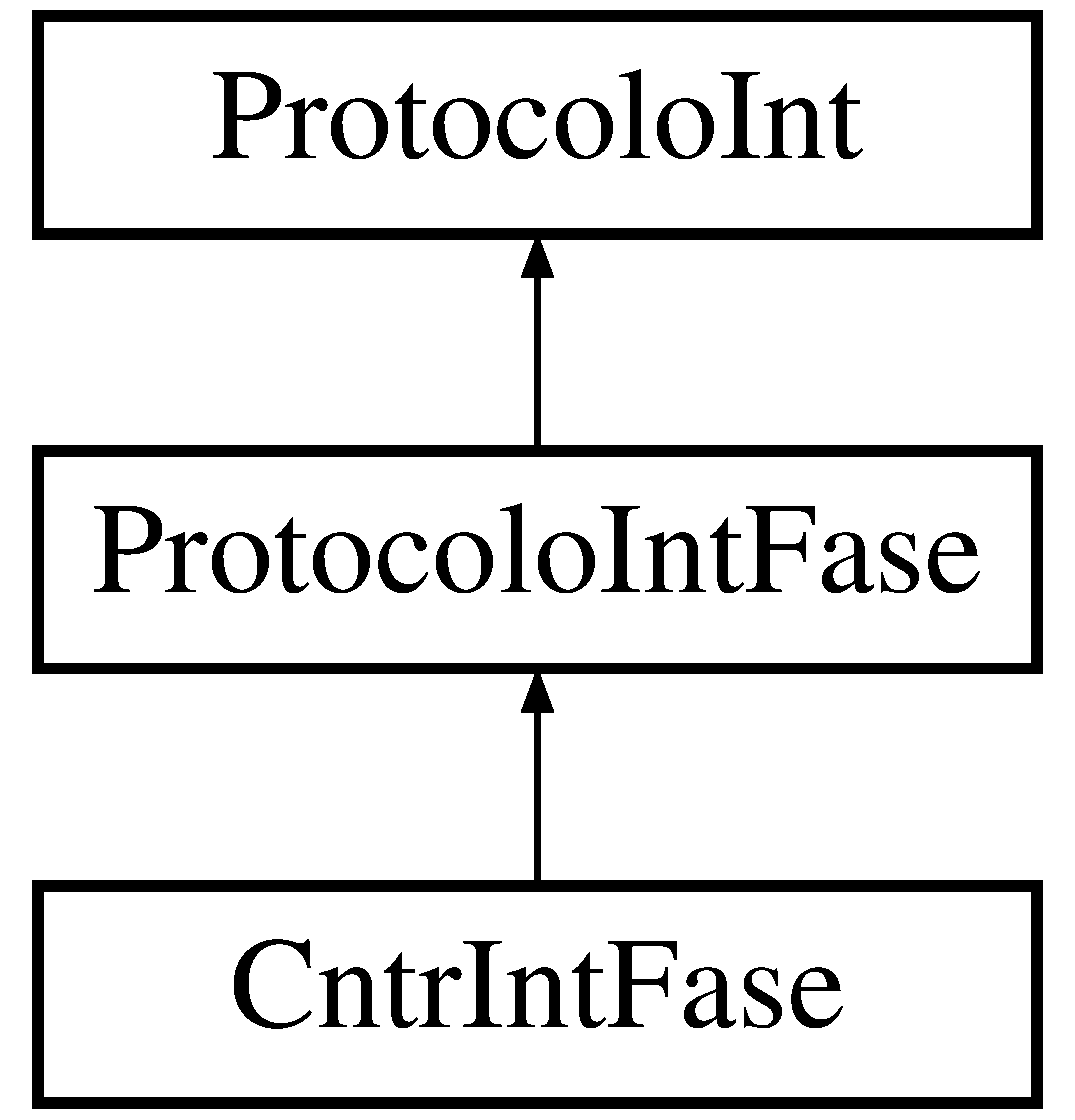
\includegraphics[height=3.000000cm]{class_cntr_int_fase}
\end{center}
\end{figure}
\subsection*{\-Membros públicos}
\begin{DoxyCompactItemize}
\item 
\hypertarget{class_cntr_int_fase_a0a48be247353d3e83c0406ed5d552aa5}{
void {\bfseries opcoes\-Fase} ()}
\label{class_cntr_int_fase_a0a48be247353d3e83c0406ed5d552aa5}

\item 
\hypertarget{class_cntr_int_fase_afe21d430453186c7a9d00cd7524a25db}{
void {\bfseries executar} ()}
\label{class_cntr_int_fase_afe21d430453186c7a9d00cd7524a25db}

\item 
void \hyperlink{class_cntr_int_fase_a51a1c838a7747917ec130c9e69b9d64b}{set\-Cntr} (\hyperlink{class_protocolo_fase}{\-Protocolo\-Fase} $\ast$)
\begin{DoxyCompactList}\small\item\em \-Seta a controladora de interacao com a \hyperlink{class_fase}{\-Fase}. \end{DoxyCompactList}\end{DoxyCompactItemize}
\subsection*{\-Atributos \-Públicos}
\begin{DoxyCompactItemize}
\item 
\hypertarget{class_cntr_int_fase_a0f718c4e96030b2724ff182b19a5be16}{
string {\bfseries codigo\-Entrada}}
\label{class_cntr_int_fase_a0f718c4e96030b2724ff182b19a5be16}

\item 
\hypertarget{class_cntr_int_fase_a3512796b953443e8e9fd93947e48553d}{
unsigned int {\bfseries tempo\-Estimado\-Entrada}}
\label{class_cntr_int_fase_a3512796b953443e8e9fd93947e48553d}

\item 
\hypertarget{class_cntr_int_fase_ac532bf08b7e575ad964138534c6feeb9}{
unsigned int {\bfseries tempo\-Efetivo\-Entrada}}
\label{class_cntr_int_fase_ac532bf08b7e575ad964138534c6feeb9}

\item 
\hypertarget{class_cntr_int_fase_af6cb3c189d0fc074e878d94900572bb6}{
\hyperlink{class_codigo___fase}{\-Codigo\-\_\-\-Fase} {\bfseries codigo\-\_\-fase}}
\label{class_cntr_int_fase_af6cb3c189d0fc074e878d94900572bb6}

\item 
\hypertarget{class_cntr_int_fase_a382a7f46bed01f2acf3b56c6bc42f917}{
\hyperlink{class_tempo}{\-Tempo} {\bfseries tempo\-\_\-estimado}}
\label{class_cntr_int_fase_a382a7f46bed01f2acf3b56c6bc42f917}

\item 
\hypertarget{class_cntr_int_fase_a4607c62f5939e390212b0907a72ff840}{
\hyperlink{class_tempo}{\-Tempo} {\bfseries tempo\-\_\-efetivo}}
\label{class_cntr_int_fase_a4607c62f5939e390212b0907a72ff840}

\end{DoxyCompactItemize}
\subsection*{\-Atributos \-Protegidos}
\begin{DoxyCompactItemize}
\item 
\hypertarget{class_cntr_int_fase_a26ae222e012957ddeb47c446b0dd2cad}{
\hyperlink{class_protocolo_fase}{\-Protocolo\-Fase} $\ast$ {\bfseries protocolo\-Fase}}
\label{class_cntr_int_fase_a26ae222e012957ddeb47c446b0dd2cad}

\end{DoxyCompactItemize}


\subsection{\-Descrição detalhada}
\-Classe que representa a controladora de interacao \-Usuario/\-Fase. 

\-Recebe a opcao escolhida pelo usuario acerca dos servicos do modulo de \hyperlink{class_fase}{\-Fase} e encaminha servico escolhido para a logica de negocio 

\subsection{\-Documentação dos métodos}
\hypertarget{class_cntr_int_fase_a51a1c838a7747917ec130c9e69b9d64b}{
\index{\-Cntr\-Int\-Fase@{\-Cntr\-Int\-Fase}!set\-Cntr@{set\-Cntr}}
\index{set\-Cntr@{set\-Cntr}!CntrIntFase@{\-Cntr\-Int\-Fase}}
\subsubsection[{set\-Cntr}]{\setlength{\rightskip}{0pt plus 5cm}void \-Cntr\-Int\-Fase\-::set\-Cntr (
\begin{DoxyParamCaption}
\item[{{\bf \-Protocolo\-Fase} $\ast$}]{protocolo\-Fase}
\end{DoxyParamCaption}
)\hspace{0.3cm}{\ttfamily  \mbox{[}inline, virtual\mbox{]}}}}
\label{class_cntr_int_fase_a51a1c838a7747917ec130c9e69b9d64b}


\-Seta a controladora de interacao com a \hyperlink{class_fase}{\-Fase}. 


\begin{DoxyParams}{\-Parâmetros}
{\em $\ast$protocolo\-Fase} & \\
\hline
\end{DoxyParams}


\-Implementa \hyperlink{class_protocolo_int_fase}{\-Protocolo\-Int\-Fase}.



\-A documentação para esta classe foi gerada a partir do seguinte ficheiro\-:\begin{DoxyCompactItemize}
\item 
\-Controladoras.\-h\end{DoxyCompactItemize}

\hypertarget{class_cntr_int_metrica}{
\section{\-Referência à classe \-Cntr\-Int\-Metrica}
\label{class_cntr_int_metrica}\index{\-Cntr\-Int\-Metrica@{\-Cntr\-Int\-Metrica}}
}


\-Classe que representa a controladora de interacao \-Usuario/\-Metrica.  




{\ttfamily \#include $<$\-Controladoras.\-h$>$}

\-Diagrama de heranças da classe \-Cntr\-Int\-Metrica\begin{figure}[H]
\begin{center}
\leavevmode
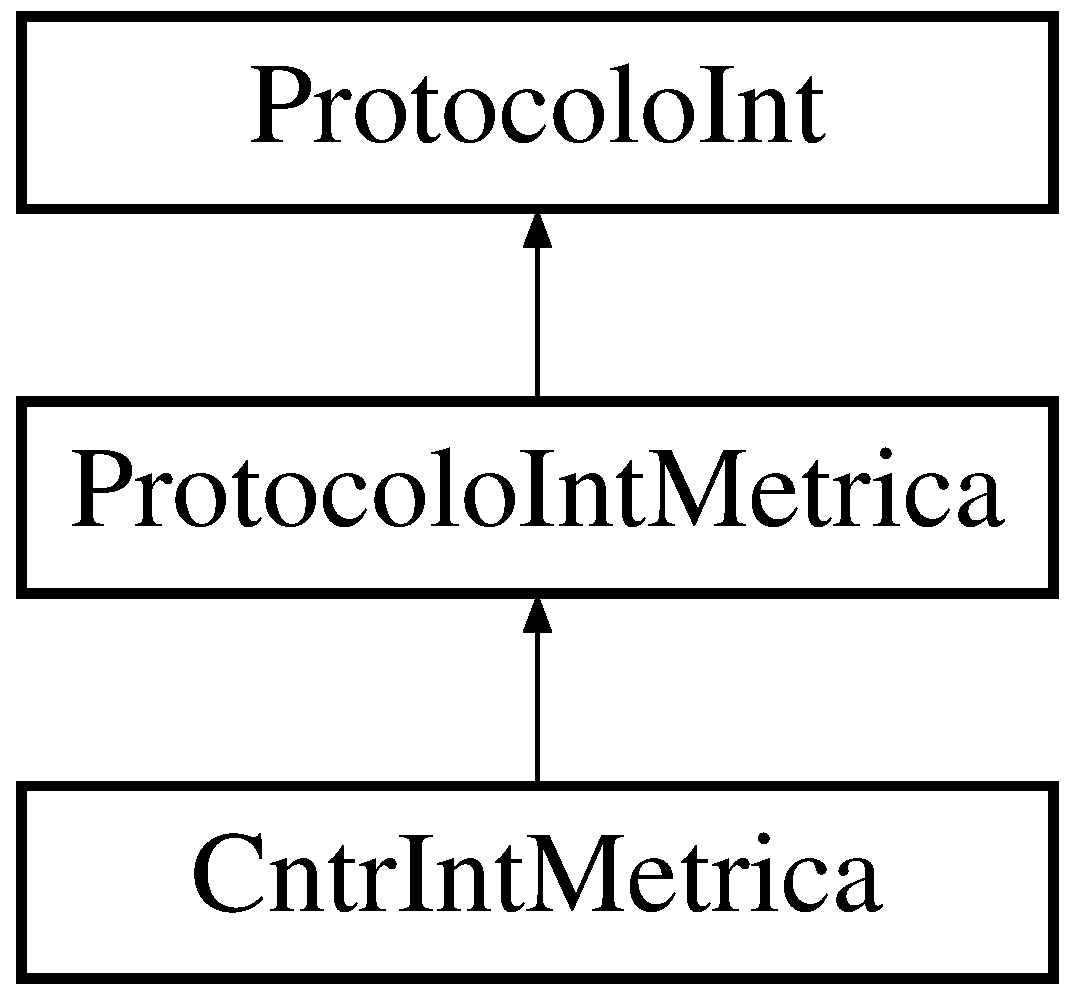
\includegraphics[height=3.000000cm]{class_cntr_int_metrica}
\end{center}
\end{figure}
\subsection*{\-Membros públicos}
\begin{DoxyCompactItemize}
\item 
\hypertarget{class_cntr_int_metrica_adbf52a7806ae74e10053c226d1a631de}{
void {\bfseries executar} ()}
\label{class_cntr_int_metrica_adbf52a7806ae74e10053c226d1a631de}

\item 
void \hyperlink{class_cntr_int_metrica_a9efa0fa35a6e7af59bebc8e6963fdc87}{set\-Cntr} (\hyperlink{class_protocolo_metrica}{\-Protocolo\-Metrica} $\ast$)
\begin{DoxyCompactList}\small\item\em \-Seta a controladora de interacao com a \hyperlink{class_metrica}{\-Metrica}. \end{DoxyCompactList}\end{DoxyCompactItemize}
\subsection*{\-Atributos \-Públicos}
\begin{DoxyCompactItemize}
\item 
\hypertarget{class_cntr_int_metrica_ae451abde34fd518505a15b143222d38f}{
string {\bfseries codigo\-Entrada}}
\label{class_cntr_int_metrica_ae451abde34fd518505a15b143222d38f}

\item 
\hypertarget{class_cntr_int_metrica_aab218b1c2f2daad9325eb16857da1463}{
string {\bfseries matricula\-Entrada}}
\label{class_cntr_int_metrica_aab218b1c2f2daad9325eb16857da1463}

\item 
\hypertarget{class_cntr_int_metrica_a202a3ddf004f9e95f296e343f25cd968}{
\hyperlink{class_codigo___projeto}{\-Codigo\-\_\-\-Projeto} {\bfseries codigo\-\_\-projeto}}
\label{class_cntr_int_metrica_a202a3ddf004f9e95f296e343f25cd968}

\item 
\hypertarget{class_cntr_int_metrica_a2a361cfc08fe506c8c9623d3ce3df6cc}{
\hyperlink{class_matricula}{\-Matricula} {\bfseries matricula}}
\label{class_cntr_int_metrica_a2a361cfc08fe506c8c9623d3ce3df6cc}

\end{DoxyCompactItemize}
\subsection*{\-Atributos \-Protegidos}
\begin{DoxyCompactItemize}
\item 
\hypertarget{class_cntr_int_metrica_a14e81b2a50fb60ef4da48ec4554d9a0c}{
\hyperlink{class_protocolo_metrica}{\-Protocolo\-Metrica} $\ast$ {\bfseries protocolo\-Metrica}}
\label{class_cntr_int_metrica_a14e81b2a50fb60ef4da48ec4554d9a0c}

\end{DoxyCompactItemize}


\subsection{\-Descrição detalhada}
\-Classe que representa a controladora de interacao \-Usuario/\-Metrica. 

\-Recebe a opcao escolhida pelo usuario acerca dos servicos do modulo de \hyperlink{class_metrica}{\-Metrica} e encaminha servico escolhido para a logica de negocio 

\subsection{\-Documentação dos métodos}
\hypertarget{class_cntr_int_metrica_a9efa0fa35a6e7af59bebc8e6963fdc87}{
\index{\-Cntr\-Int\-Metrica@{\-Cntr\-Int\-Metrica}!set\-Cntr@{set\-Cntr}}
\index{set\-Cntr@{set\-Cntr}!CntrIntMetrica@{\-Cntr\-Int\-Metrica}}
\subsubsection[{set\-Cntr}]{\setlength{\rightskip}{0pt plus 5cm}void \-Cntr\-Int\-Metrica\-::set\-Cntr (
\begin{DoxyParamCaption}
\item[{{\bf \-Protocolo\-Metrica} $\ast$}]{protocolo\-Metrica}
\end{DoxyParamCaption}
)\hspace{0.3cm}{\ttfamily  \mbox{[}inline, virtual\mbox{]}}}}
\label{class_cntr_int_metrica_a9efa0fa35a6e7af59bebc8e6963fdc87}


\-Seta a controladora de interacao com a \hyperlink{class_metrica}{\-Metrica}. 


\begin{DoxyParams}{\-Parâmetros}
{\em $\ast$protocolo\-Metrica} & \\
\hline
\end{DoxyParams}


\-Implementa \hyperlink{class_protocolo_int_metrica}{\-Protocolo\-Int\-Metrica}.



\-A documentação para esta classe foi gerada a partir do seguinte ficheiro\-:\begin{DoxyCompactItemize}
\item 
\-Controladoras.\-h\end{DoxyCompactItemize}

\hypertarget{class_cntr_int_modulo}{
\section{\-Referência à classe \-Cntr\-Int\-Modulo}
\label{class_cntr_int_modulo}\index{\-Cntr\-Int\-Modulo@{\-Cntr\-Int\-Modulo}}
}


\-Classe que representa a controladora de interacao \-Usuario/\-Modulo.  




{\ttfamily \#include $<$\-Controladoras.\-h$>$}

\-Diagrama de heranças da classe \-Cntr\-Int\-Modulo\begin{figure}[H]
\begin{center}
\leavevmode
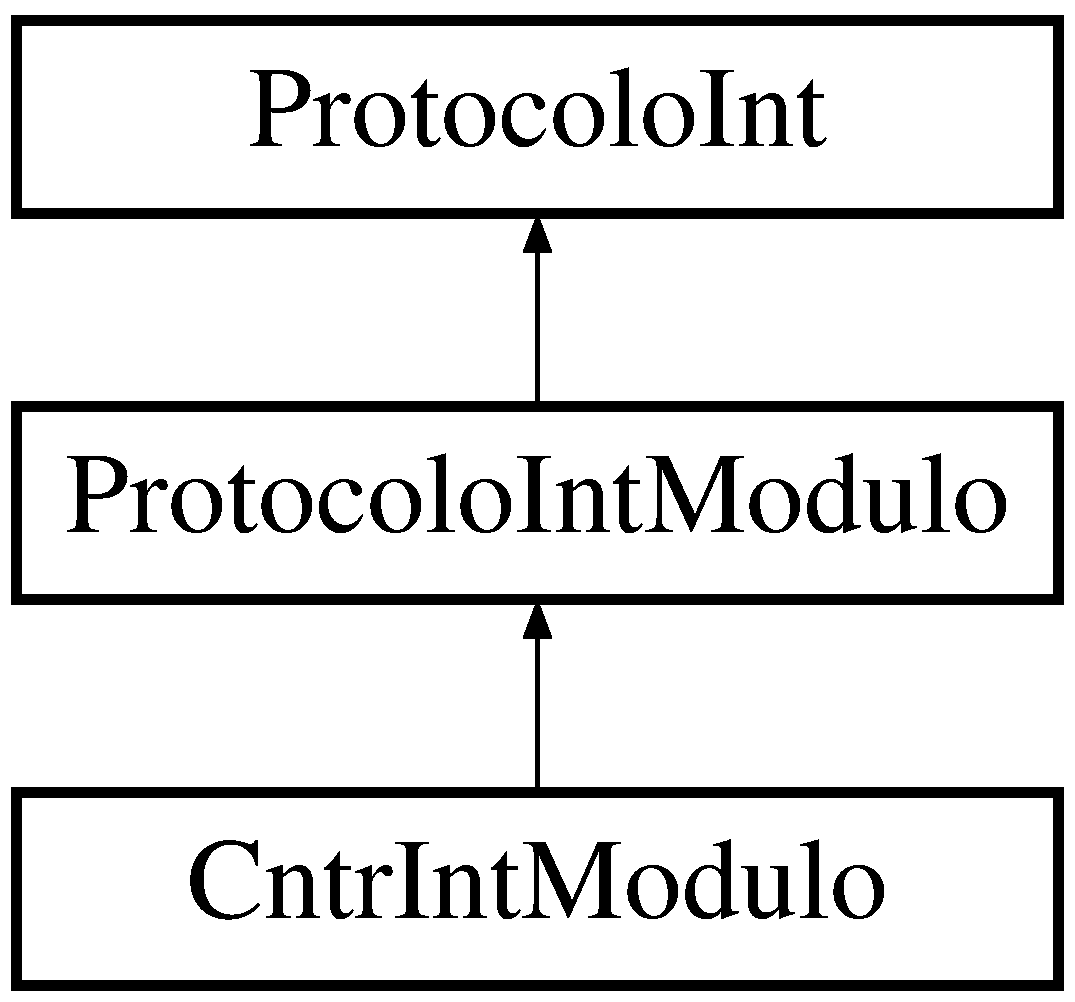
\includegraphics[height=3.000000cm]{class_cntr_int_modulo}
\end{center}
\end{figure}
\subsection*{\-Membros públicos}
\begin{DoxyCompactItemize}
\item 
\hypertarget{class_cntr_int_modulo_a7c6fb782e81f2585cc5c45b3416eca9e}{
void {\bfseries executar} ()}
\label{class_cntr_int_modulo_a7c6fb782e81f2585cc5c45b3416eca9e}

\item 
void \hyperlink{class_cntr_int_modulo_a4233eefb24e6578b004bfe5d00bad190}{set\-Cntr} (\hyperlink{class_protocolo_modulo}{\-Protocolo\-Modulo} $\ast$)
\begin{DoxyCompactList}\small\item\em \-Seta a controladora de interacao com o modulo. \end{DoxyCompactList}\end{DoxyCompactItemize}
\subsection*{\-Atributos \-Públicos}
\begin{DoxyCompactItemize}
\item 
\hypertarget{class_cntr_int_modulo_a1eb1b5c91e5b3e28dc0b942df1e3f1f7}{
string {\bfseries codigo\-Entrada}}
\label{class_cntr_int_modulo_a1eb1b5c91e5b3e28dc0b942df1e3f1f7}

\item 
\hypertarget{class_cntr_int_modulo_aff726cb02945c2693475c581d2394aca}{
string {\bfseries nome\-Entrada}}
\label{class_cntr_int_modulo_aff726cb02945c2693475c581d2394aca}

\item 
\hypertarget{class_cntr_int_modulo_a5c90af3779e73cb954659aa7c7dca322}{
unsigned int {\bfseries tamanho\-Entrada}}
\label{class_cntr_int_modulo_a5c90af3779e73cb954659aa7c7dca322}

\item 
\hypertarget{class_cntr_int_modulo_a6def2162909614ff31f6719ee97ac952}{
\hyperlink{class_codigo___modulo}{\-Codigo\-\_\-\-Modulo} {\bfseries codigo\-\_\-modulo}}
\label{class_cntr_int_modulo_a6def2162909614ff31f6719ee97ac952}

\item 
\hypertarget{class_cntr_int_modulo_a94d5c230b0f15f16aa9484924665e1e6}{
\hyperlink{class_nome___arquivo}{\-Nome\-\_\-\-Arquivo} {\bfseries nome\-\_\-arquivo}}
\label{class_cntr_int_modulo_a94d5c230b0f15f16aa9484924665e1e6}

\item 
\hypertarget{class_cntr_int_modulo_a4a54d3d19836141c6c8d9a8fdb8e4777}{
\hyperlink{class_tamanho}{\-Tamanho} {\bfseries tamanho}}
\label{class_cntr_int_modulo_a4a54d3d19836141c6c8d9a8fdb8e4777}

\end{DoxyCompactItemize}
\subsection*{\-Atributos \-Protegidos}
\begin{DoxyCompactItemize}
\item 
\hypertarget{class_cntr_int_modulo_a814c981835b26c196cb0df7c18456485}{
\hyperlink{class_protocolo_modulo}{\-Protocolo\-Modulo} $\ast$ {\bfseries protocolo\-Modulo}}
\label{class_cntr_int_modulo_a814c981835b26c196cb0df7c18456485}

\end{DoxyCompactItemize}


\subsection{\-Descrição detalhada}
\-Classe que representa a controladora de interacao \-Usuario/\-Modulo. 

\-Recebe a opcao escolhida pelo usuario acerca dos servicos do \hyperlink{class_modulo}{\-Modulo} e encaminha servico escolhido para a logica de negocio 

\subsection{\-Documentação dos métodos}
\hypertarget{class_cntr_int_modulo_a4233eefb24e6578b004bfe5d00bad190}{
\index{\-Cntr\-Int\-Modulo@{\-Cntr\-Int\-Modulo}!set\-Cntr@{set\-Cntr}}
\index{set\-Cntr@{set\-Cntr}!CntrIntModulo@{\-Cntr\-Int\-Modulo}}
\subsubsection[{set\-Cntr}]{\setlength{\rightskip}{0pt plus 5cm}void \-Cntr\-Int\-Modulo\-::set\-Cntr (
\begin{DoxyParamCaption}
\item[{{\bf \-Protocolo\-Modulo} $\ast$}]{protocolo\-Modulo}
\end{DoxyParamCaption}
)\hspace{0.3cm}{\ttfamily  \mbox{[}inline, virtual\mbox{]}}}}
\label{class_cntr_int_modulo_a4233eefb24e6578b004bfe5d00bad190}


\-Seta a controladora de interacao com o modulo. 


\begin{DoxyParams}{\-Parâmetros}
{\em $\ast$protocolo\-Modulo} & \\
\hline
\end{DoxyParams}


\-Implementa \hyperlink{class_protocolo_int_modulo}{\-Protocolo\-Int\-Modulo}.



\-A documentação para esta classe foi gerada a partir do seguinte ficheiro\-:\begin{DoxyCompactItemize}
\item 
\-Controladoras.\-h\end{DoxyCompactItemize}

\hypertarget{class_cntr_int_navegacao}{
\section{\-Referência à classe \-Cntr\-Int\-Navegacao}
\label{class_cntr_int_navegacao}\index{\-Cntr\-Int\-Navegacao@{\-Cntr\-Int\-Navegacao}}
}


\-Classe que representa a controladora de interacao \-Usuario/\-Navegacao.  




{\ttfamily \#include $<$\-Controladoras.\-h$>$}

\subsection*{\-Membros públicos}
\begin{DoxyCompactItemize}
\item 
void \hyperlink{class_cntr_int_navegacao_a8c5acb2786391f283f06d96cfb359ab9}{set\-Cntr\-Int\-Projeto} (\hyperlink{class_protocolo_int}{\-Protocolo\-Int} $\ast$)
\begin{DoxyCompactList}\small\item\em \-Seta a controladora de interacao da navegacao com o \hyperlink{class_projeto}{\-Projeto}. \end{DoxyCompactList}\item 
void \hyperlink{class_cntr_int_navegacao_a805d37d1d5c82a6f6d8e2cf3fb4805a0}{set\-Cntr\-Int\-Modulo} (\hyperlink{class_protocolo_int}{\-Protocolo\-Int} $\ast$)
\begin{DoxyCompactList}\small\item\em \-Seta a controladora de interacao da navegacao com o \hyperlink{class_modulo}{\-Modulo}. \end{DoxyCompactList}\item 
void \hyperlink{class_cntr_int_navegacao_a74b99352a7228af917b559436a97a288}{set\-Cntr\-Int\-Fase} (\hyperlink{class_protocolo_int}{\-Protocolo\-Int} $\ast$)
\begin{DoxyCompactList}\small\item\em \-Seta a controladora de interacao da navegacao com a \hyperlink{class_fase}{\-Fase}. \end{DoxyCompactList}\item 
void \hyperlink{class_cntr_int_navegacao_ad46a81e7428712d4fdeeadbb6a706797}{set\-Cntr\-Int\-Metrica} (\hyperlink{class_protocolo_int}{\-Protocolo\-Int} $\ast$)
\begin{DoxyCompactList}\small\item\em \-Seta a controladora de interacao da navegacao com a \hyperlink{class_metrica}{\-Metrica}. \end{DoxyCompactList}\item 
\hypertarget{class_cntr_int_navegacao_a0a5f1f1b0606b7379bb84f855a397519}{
void {\bfseries executar} ()}
\label{class_cntr_int_navegacao_a0a5f1f1b0606b7379bb84f855a397519}

\end{DoxyCompactItemize}
\subsection*{\-Atributos \-Protegidos}
\begin{DoxyCompactItemize}
\item 
\hypertarget{class_cntr_int_navegacao_a762aaa9e29e2184257312a65eea2859c}{
\hyperlink{class_protocolo_int}{\-Protocolo\-Int} $\ast$ {\bfseries protocolo\-Int\-Projeto}}
\label{class_cntr_int_navegacao_a762aaa9e29e2184257312a65eea2859c}

\item 
\hypertarget{class_cntr_int_navegacao_acadf3fb9694d58b5b86ac94df30af7b5}{
\hyperlink{class_protocolo_int}{\-Protocolo\-Int} $\ast$ {\bfseries protocolo\-Int\-Modulo}}
\label{class_cntr_int_navegacao_acadf3fb9694d58b5b86ac94df30af7b5}

\item 
\hypertarget{class_cntr_int_navegacao_a235053554e87b568a599834f190bc82b}{
\hyperlink{class_protocolo_int}{\-Protocolo\-Int} $\ast$ {\bfseries protocolo\-Int\-Fase}}
\label{class_cntr_int_navegacao_a235053554e87b568a599834f190bc82b}

\item 
\hypertarget{class_cntr_int_navegacao_a68cde9fb9e3782b621e37b587e64b25e}{
\hyperlink{class_protocolo_int}{\-Protocolo\-Int} $\ast$ {\bfseries protocolo\-Int\-Metrica}}
\label{class_cntr_int_navegacao_a68cde9fb9e3782b621e37b587e64b25e}

\end{DoxyCompactItemize}


\subsection{\-Descrição detalhada}
\-Classe que representa a controladora de interacao \-Usuario/\-Navegacao. 

\-Recebe a opcao escolhida pelo usuario e encaminha servico para a classe controladora escolhida escolha do usu�rio, atraves do set do \hyperlink{class_protocolo_int}{\-Protocolo\-Int} especifico 

\subsection{\-Documentação dos métodos}
\hypertarget{class_cntr_int_navegacao_a74b99352a7228af917b559436a97a288}{
\index{\-Cntr\-Int\-Navegacao@{\-Cntr\-Int\-Navegacao}!set\-Cntr\-Int\-Fase@{set\-Cntr\-Int\-Fase}}
\index{set\-Cntr\-Int\-Fase@{set\-Cntr\-Int\-Fase}!CntrIntNavegacao@{\-Cntr\-Int\-Navegacao}}
\subsubsection[{set\-Cntr\-Int\-Fase}]{\setlength{\rightskip}{0pt plus 5cm}void \-Cntr\-Int\-Navegacao\-::set\-Cntr\-Int\-Fase (
\begin{DoxyParamCaption}
\item[{{\bf \-Protocolo\-Int} $\ast$}]{cntr}
\end{DoxyParamCaption}
)\hspace{0.3cm}{\ttfamily  \mbox{[}inline\mbox{]}}}}
\label{class_cntr_int_navegacao_a74b99352a7228af917b559436a97a288}


\-Seta a controladora de interacao da navegacao com a \hyperlink{class_fase}{\-Fase}. 


\begin{DoxyParams}{\-Parâmetros}
{\em $\ast$protocolo\-Int\-Fase} & \\
\hline
\end{DoxyParams}
\hypertarget{class_cntr_int_navegacao_ad46a81e7428712d4fdeeadbb6a706797}{
\index{\-Cntr\-Int\-Navegacao@{\-Cntr\-Int\-Navegacao}!set\-Cntr\-Int\-Metrica@{set\-Cntr\-Int\-Metrica}}
\index{set\-Cntr\-Int\-Metrica@{set\-Cntr\-Int\-Metrica}!CntrIntNavegacao@{\-Cntr\-Int\-Navegacao}}
\subsubsection[{set\-Cntr\-Int\-Metrica}]{\setlength{\rightskip}{0pt plus 5cm}void \-Cntr\-Int\-Navegacao\-::set\-Cntr\-Int\-Metrica (
\begin{DoxyParamCaption}
\item[{{\bf \-Protocolo\-Int} $\ast$}]{cntr}
\end{DoxyParamCaption}
)\hspace{0.3cm}{\ttfamily  \mbox{[}inline\mbox{]}}}}
\label{class_cntr_int_navegacao_ad46a81e7428712d4fdeeadbb6a706797}


\-Seta a controladora de interacao da navegacao com a \hyperlink{class_metrica}{\-Metrica}. 


\begin{DoxyParams}{\-Parâmetros}
{\em $\ast$protocolo\-Int\-Metrica} & \\
\hline
\end{DoxyParams}
\hypertarget{class_cntr_int_navegacao_a805d37d1d5c82a6f6d8e2cf3fb4805a0}{
\index{\-Cntr\-Int\-Navegacao@{\-Cntr\-Int\-Navegacao}!set\-Cntr\-Int\-Modulo@{set\-Cntr\-Int\-Modulo}}
\index{set\-Cntr\-Int\-Modulo@{set\-Cntr\-Int\-Modulo}!CntrIntNavegacao@{\-Cntr\-Int\-Navegacao}}
\subsubsection[{set\-Cntr\-Int\-Modulo}]{\setlength{\rightskip}{0pt plus 5cm}void \-Cntr\-Int\-Navegacao\-::set\-Cntr\-Int\-Modulo (
\begin{DoxyParamCaption}
\item[{{\bf \-Protocolo\-Int} $\ast$}]{cntr}
\end{DoxyParamCaption}
)\hspace{0.3cm}{\ttfamily  \mbox{[}inline\mbox{]}}}}
\label{class_cntr_int_navegacao_a805d37d1d5c82a6f6d8e2cf3fb4805a0}


\-Seta a controladora de interacao da navegacao com o \hyperlink{class_modulo}{\-Modulo}. 


\begin{DoxyParams}{\-Parâmetros}
{\em $\ast$protocolo\-Int\-Modulo} & \\
\hline
\end{DoxyParams}
\hypertarget{class_cntr_int_navegacao_a8c5acb2786391f283f06d96cfb359ab9}{
\index{\-Cntr\-Int\-Navegacao@{\-Cntr\-Int\-Navegacao}!set\-Cntr\-Int\-Projeto@{set\-Cntr\-Int\-Projeto}}
\index{set\-Cntr\-Int\-Projeto@{set\-Cntr\-Int\-Projeto}!CntrIntNavegacao@{\-Cntr\-Int\-Navegacao}}
\subsubsection[{set\-Cntr\-Int\-Projeto}]{\setlength{\rightskip}{0pt plus 5cm}void \-Cntr\-Int\-Navegacao\-::set\-Cntr\-Int\-Projeto (
\begin{DoxyParamCaption}
\item[{{\bf \-Protocolo\-Int} $\ast$}]{cntr}
\end{DoxyParamCaption}
)\hspace{0.3cm}{\ttfamily  \mbox{[}inline\mbox{]}}}}
\label{class_cntr_int_navegacao_a8c5acb2786391f283f06d96cfb359ab9}


\-Seta a controladora de interacao da navegacao com o \hyperlink{class_projeto}{\-Projeto}. 


\begin{DoxyParams}{\-Parâmetros}
{\em $\ast$protocolo\-Int\-Projeto} & \\
\hline
\end{DoxyParams}


\-A documentação para esta classe foi gerada a partir do seguinte ficheiro\-:\begin{DoxyCompactItemize}
\item 
\-Controladoras.\-h\end{DoxyCompactItemize}

\hypertarget{class_cntr_int_projeto}{
\section{\-Referência à classe \-Cntr\-Int\-Projeto}
\label{class_cntr_int_projeto}\index{\-Cntr\-Int\-Projeto@{\-Cntr\-Int\-Projeto}}
}


\-Classe que representa a controladora de interacao \-Usuario/\-Projeto.  




{\ttfamily \#include $<$\-Controladoras.\-h$>$}

\-Diagrama de heranças da classe \-Cntr\-Int\-Projeto\begin{figure}[H]
\begin{center}
\leavevmode
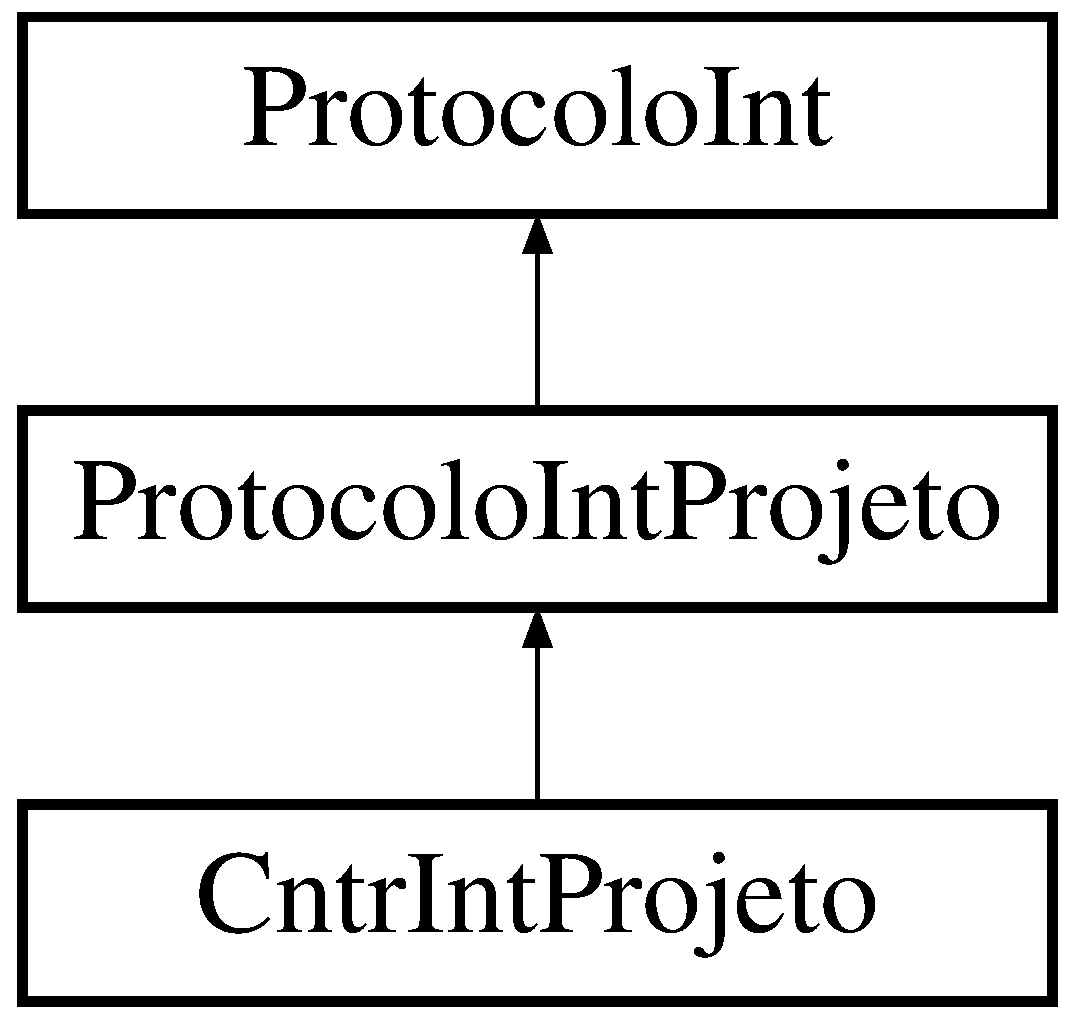
\includegraphics[height=3.000000cm]{class_cntr_int_projeto}
\end{center}
\end{figure}
\subsection*{\-Membros públicos}
\begin{DoxyCompactItemize}
\item 
\hypertarget{class_cntr_int_projeto_ab6de5c18ab98d4bcb3cb5413a7f5cf00}{
void {\bfseries executar} ()}
\label{class_cntr_int_projeto_ab6de5c18ab98d4bcb3cb5413a7f5cf00}

\item 
void \hyperlink{class_cntr_int_projeto_a21952091898e3d965af084ecbec78301}{set\-Cntr} (\hyperlink{class_protocolo_projeto}{\-Protocolo\-Projeto} $\ast$)
\begin{DoxyCompactList}\small\item\em \-Seta a controladora de interacao com o projeto. \end{DoxyCompactList}\end{DoxyCompactItemize}
\subsection*{\-Atributos \-Públicos}
\begin{DoxyCompactItemize}
\item 
\hypertarget{class_cntr_int_projeto_a8da6e2ac1d9452d3965cb64b4863c0bc}{
string {\bfseries matricula\-Entrada}}
\label{class_cntr_int_projeto_a8da6e2ac1d9452d3965cb64b4863c0bc}

\item 
\hypertarget{class_cntr_int_projeto_acf3904d1d7d0abd881dd63981c7cd1b1}{
string {\bfseries codigo\-Entrada}}
\label{class_cntr_int_projeto_acf3904d1d7d0abd881dd63981c7cd1b1}

\item 
\hypertarget{class_cntr_int_projeto_aa99c8ae9536f4b378acb8c29211a0ee7}{
unsigned int {\bfseries data\-Inicio\-Entrada}}
\label{class_cntr_int_projeto_aa99c8ae9536f4b378acb8c29211a0ee7}

\item 
\hypertarget{class_cntr_int_projeto_a8e3049a0271272cc00120131db765464}{
unsigned int {\bfseries data\-Termino\-Entrada}}
\label{class_cntr_int_projeto_a8e3049a0271272cc00120131db765464}

\item 
\hypertarget{class_cntr_int_projeto_aa1e874ee3f9875321a6c52abd18a9595}{
unsigned int {\bfseries nota\-Entrada}}
\label{class_cntr_int_projeto_aa1e874ee3f9875321a6c52abd18a9595}

\item 
\hypertarget{class_cntr_int_projeto_a2858846b000b7e54776256c1be606877}{
\hyperlink{class_matricula}{\-Matricula} {\bfseries matricula}}
\label{class_cntr_int_projeto_a2858846b000b7e54776256c1be606877}

\item 
\hypertarget{class_cntr_int_projeto_a9c54b1af9c555e76501e3b0c3304c9a1}{
\hyperlink{class_codigo___projeto}{\-Codigo\-\_\-\-Projeto} {\bfseries codigo\-\_\-projeto}}
\label{class_cntr_int_projeto_a9c54b1af9c555e76501e3b0c3304c9a1}

\item 
\hypertarget{class_cntr_int_projeto_ac53a3e721c04a9c4a72201d65a19a778}{
\hyperlink{class_data___inicio}{\-Data\-\_\-\-Inicio} {\bfseries data\-\_\-inicio}}
\label{class_cntr_int_projeto_ac53a3e721c04a9c4a72201d65a19a778}

\item 
\hypertarget{class_cntr_int_projeto_ab30ed341c5bf93a96dc0f04ff719ddee}{
\hyperlink{class_data___termino}{\-Data\-\_\-\-Termino} {\bfseries data\-\_\-termino}}
\label{class_cntr_int_projeto_ab30ed341c5bf93a96dc0f04ff719ddee}

\item 
\hypertarget{class_cntr_int_projeto_a47bd294d19f70c3afda8ce99e65b959e}{
\hyperlink{class_nota}{\-Nota} {\bfseries nota}}
\label{class_cntr_int_projeto_a47bd294d19f70c3afda8ce99e65b959e}

\end{DoxyCompactItemize}
\subsection*{\-Atributos \-Protegidos}
\begin{DoxyCompactItemize}
\item 
\hypertarget{class_cntr_int_projeto_a242c6381f8f0d0b2b7130b0c3af0afee}{
\hyperlink{class_protocolo_projeto}{\-Protocolo\-Projeto} $\ast$ {\bfseries protocolo\-Projeto}}
\label{class_cntr_int_projeto_a242c6381f8f0d0b2b7130b0c3af0afee}

\end{DoxyCompactItemize}


\subsection{\-Descrição detalhada}
\-Classe que representa a controladora de interacao \-Usuario/\-Projeto. 

\-Recebe a opcao escolhida pelo usuario acerca dos servicos do modulo de \hyperlink{class_projeto}{\-Projeto} e encaminha servico escolhido para a logica de negocio 

\subsection{\-Documentação dos métodos}
\hypertarget{class_cntr_int_projeto_a21952091898e3d965af084ecbec78301}{
\index{\-Cntr\-Int\-Projeto@{\-Cntr\-Int\-Projeto}!set\-Cntr@{set\-Cntr}}
\index{set\-Cntr@{set\-Cntr}!CntrIntProjeto@{\-Cntr\-Int\-Projeto}}
\subsubsection[{set\-Cntr}]{\setlength{\rightskip}{0pt plus 5cm}void \-Cntr\-Int\-Projeto\-::set\-Cntr (
\begin{DoxyParamCaption}
\item[{{\bf \-Protocolo\-Projeto} $\ast$}]{protocolo\-Projeto}
\end{DoxyParamCaption}
)\hspace{0.3cm}{\ttfamily  \mbox{[}inline, virtual\mbox{]}}}}
\label{class_cntr_int_projeto_a21952091898e3d965af084ecbec78301}


\-Seta a controladora de interacao com o projeto. 


\begin{DoxyParams}{\-Parâmetros}
{\em $\ast$protocolo\-Projeto} & \\
\hline
\end{DoxyParams}


\-Implementa \hyperlink{class_protocolo_int_projeto}{\-Protocolo\-Int\-Projeto}.



\-A documentação para esta classe foi gerada a partir do seguinte ficheiro\-:\begin{DoxyCompactItemize}
\item 
\-Controladoras.\-h\end{DoxyCompactItemize}

\hypertarget{class_codigo___fase}{
\section{\-Referência da \-Classe \-Codigo\-\_\-\-Fase}
\label{class_codigo___fase}\index{\-Codigo\-\_\-\-Fase@{\-Codigo\-\_\-\-Fase}}
}


\-Classe que representa o dominio \hyperlink{class_codigo___fase}{\-Codigo\-\_\-\-Fase}.  




{\ttfamily \#include $<$\-Dominios.\-h$>$}

\subsection*{\-Métodos \-Públicos}
\begin{DoxyCompactItemize}
\item 
\hypertarget{class_codigo___fase_a95e4aaa46eb3c9508216d9914f10de9b}{
{\bfseries \-Codigo\-\_\-\-Fase} (string)  throw (invalid\-\_\-argument)}
\label{class_codigo___fase_a95e4aaa46eb3c9508216d9914f10de9b}

\item 
void \hyperlink{class_codigo___fase_a30ddd9595c79d2ba10d25a857ae01704}{set\-Valor} (const string \&)  throw (invalid\-\_\-argument)
\begin{DoxyCompactList}\small\item\em \-Seta o valor de \-Codigo de \hyperlink{class_fase}{\-Fase}. \end{DoxyCompactList}\item 
string \hyperlink{class_codigo___fase_ad6211e7c092a64788fe6b007addd48d3}{get\-Valor} () const 
\begin{DoxyCompactList}\small\item\em \-Retorna o valor de \-Codigo de \hyperlink{class_fase}{\-Fase}. \end{DoxyCompactList}\end{DoxyCompactItemize}


\subsection{\-Descrição \-Detalhada}
\-Classe que representa o dominio \hyperlink{class_codigo___fase}{\-Codigo\-\_\-\-Fase}. 

\-Armazena os atributos de \-Codigo \-De \hyperlink{class_fase}{\-Fase} apos validacao\-: numero decimal composto por 1 digito 

\subsection{\-Métodos}
\hypertarget{class_codigo___fase_ad6211e7c092a64788fe6b007addd48d3}{
\index{\-Codigo\-\_\-\-Fase@{\-Codigo\-\_\-\-Fase}!get\-Valor@{get\-Valor}}
\index{get\-Valor@{get\-Valor}!Codigo_Fase@{\-Codigo\-\_\-\-Fase}}
\subsubsection[{get\-Valor}]{\setlength{\rightskip}{0pt plus 5cm}string \-Codigo\-\_\-\-Fase\-::get\-Valor (
\begin{DoxyParamCaption}
{}
\end{DoxyParamCaption}
) const\hspace{0.3cm}{\ttfamily  \mbox{[}inline\mbox{]}}}}
\label{class_codigo___fase_ad6211e7c092a64788fe6b007addd48d3}


\-Retorna o valor de \-Codigo de \hyperlink{class_fase}{\-Fase}. 

\begin{DoxyReturn}{\-Retorna}
valor 
\end{DoxyReturn}
\hypertarget{class_codigo___fase_a30ddd9595c79d2ba10d25a857ae01704}{
\index{\-Codigo\-\_\-\-Fase@{\-Codigo\-\_\-\-Fase}!set\-Valor@{set\-Valor}}
\index{set\-Valor@{set\-Valor}!Codigo_Fase@{\-Codigo\-\_\-\-Fase}}
\subsubsection[{set\-Valor}]{\setlength{\rightskip}{0pt plus 5cm}void \-Codigo\-\_\-\-Fase\-::set\-Valor (
\begin{DoxyParamCaption}
\item[{const string \&}]{valor}
\end{DoxyParamCaption}
)  throw (invalid\-\_\-argument)\hspace{0.3cm}{\ttfamily  \mbox{[}inline\mbox{]}}}}
\label{class_codigo___fase_a30ddd9595c79d2ba10d25a857ae01704}


\-Seta o valor de \-Codigo de \hyperlink{class_fase}{\-Fase}. 


\begin{DoxyParams}{\-Parâmetros}
{\em valor} & \\
\hline
\end{DoxyParams}


\-A documentação para esta classe foi gerada a partir do seguinte arquivo\-:\begin{DoxyCompactItemize}
\item 
header/\-Dominios.\-h\end{DoxyCompactItemize}

\hypertarget{class_codigo___modulo}{
\section{\-Referência à classe \-Codigo\-\_\-\-Modulo}
\label{class_codigo___modulo}\index{\-Codigo\-\_\-\-Modulo@{\-Codigo\-\_\-\-Modulo}}
}


\-Classe que representa o dominio \hyperlink{class_codigo___modulo}{\-Codigo\-\_\-\-Modulo}.  




{\ttfamily \#include $<$\-Dominios.\-h$>$}

\subsection*{\-Membros públicos}
\begin{DoxyCompactItemize}
\item 
\hypertarget{class_codigo___modulo_af02fd77a63061429f2951bc78741093e}{
{\bfseries \-Codigo\-\_\-\-Modulo} (string)  throw (invalid\-\_\-argument)}
\label{class_codigo___modulo_af02fd77a63061429f2951bc78741093e}

\item 
void \hyperlink{class_codigo___modulo_a974ed9c3733dcf75c362c53653e407e7}{set\-Valor} (const string \&)  throw (invalid\-\_\-argument)
\begin{DoxyCompactList}\small\item\em \-Seta o valor de \-Codigo de \hyperlink{class_modulo}{\-Modulo}. \end{DoxyCompactList}\item 
string \hyperlink{class_codigo___modulo_a87112e0fb26a7d32fe8cb06cc7d32746}{get\-Valor} () const 
\begin{DoxyCompactList}\small\item\em \-Retorna o valor de \-Codigo de \hyperlink{class_modulo}{\-Modulo}. \end{DoxyCompactList}\end{DoxyCompactItemize}


\subsection{\-Descrição detalhada}
\-Classe que representa o dominio \hyperlink{class_codigo___modulo}{\-Codigo\-\_\-\-Modulo}. 

\-Armazena os atributos de \-Codigo \-De \hyperlink{class_modulo}{\-Modulo} apos validacao\-: numero decimal composto por 5 digitos 

\subsection{\-Documentação dos métodos}
\hypertarget{class_codigo___modulo_a87112e0fb26a7d32fe8cb06cc7d32746}{
\index{\-Codigo\-\_\-\-Modulo@{\-Codigo\-\_\-\-Modulo}!get\-Valor@{get\-Valor}}
\index{get\-Valor@{get\-Valor}!Codigo_Modulo@{\-Codigo\-\_\-\-Modulo}}
\subsubsection[{get\-Valor}]{\setlength{\rightskip}{0pt plus 5cm}string \-Codigo\-\_\-\-Modulo\-::get\-Valor (
\begin{DoxyParamCaption}
{}
\end{DoxyParamCaption}
) const\hspace{0.3cm}{\ttfamily  \mbox{[}inline\mbox{]}}}}
\label{class_codigo___modulo_a87112e0fb26a7d32fe8cb06cc7d32746}


\-Retorna o valor de \-Codigo de \hyperlink{class_modulo}{\-Modulo}. 

\begin{DoxyReturn}{\-Retorna}
valor 
\end{DoxyReturn}
\hypertarget{class_codigo___modulo_a974ed9c3733dcf75c362c53653e407e7}{
\index{\-Codigo\-\_\-\-Modulo@{\-Codigo\-\_\-\-Modulo}!set\-Valor@{set\-Valor}}
\index{set\-Valor@{set\-Valor}!Codigo_Modulo@{\-Codigo\-\_\-\-Modulo}}
\subsubsection[{set\-Valor}]{\setlength{\rightskip}{0pt plus 5cm}void \-Codigo\-\_\-\-Modulo\-::set\-Valor (
\begin{DoxyParamCaption}
\item[{const string \&}]{valor}
\end{DoxyParamCaption}
)  throw (invalid\-\_\-argument)\hspace{0.3cm}{\ttfamily  \mbox{[}inline\mbox{]}}}}
\label{class_codigo___modulo_a974ed9c3733dcf75c362c53653e407e7}


\-Seta o valor de \-Codigo de \hyperlink{class_modulo}{\-Modulo}. 


\begin{DoxyParams}{\-Parâmetros}
{\em valor} & \\
\hline
\end{DoxyParams}


\-A documentação para esta classe foi gerada a partir do seguinte ficheiro\-:\begin{DoxyCompactItemize}
\item 
\-Dominios.\-h\end{DoxyCompactItemize}

\hypertarget{class_codigo___projeto}{
\section{\-Referência da \-Classe \-Codigo\-\_\-\-Projeto}
\label{class_codigo___projeto}\index{\-Codigo\-\_\-\-Projeto@{\-Codigo\-\_\-\-Projeto}}
}


\-Classe que representa o dominio \hyperlink{class_codigo___projeto}{\-Codigo\-\_\-\-Projeto}.  




{\ttfamily \#include $<$\-Dominios.\-h$>$}

\subsection*{\-Métodos \-Públicos}
\begin{DoxyCompactItemize}
\item 
\hypertarget{class_codigo___projeto_ac3aaa481366d852d0c654bac3f95bc97}{
{\bfseries \-Codigo\-\_\-\-Projeto} (string)  throw (invalid\-\_\-argument)}
\label{class_codigo___projeto_ac3aaa481366d852d0c654bac3f95bc97}

\item 
void \hyperlink{class_codigo___projeto_a8628c9fa45bb9be7c4b25ebfbe2c255c}{set\-Valor} (const string \&)  throw (invalid\-\_\-argument)
\begin{DoxyCompactList}\small\item\em \-Seta o valor de \-Codigo de \hyperlink{class_projeto}{\-Projeto}. \end{DoxyCompactList}\item 
string \hyperlink{class_codigo___projeto_ae2a6a32b20fcdd82dbafeef8cbec5bb2}{get\-Valor} () const 
\begin{DoxyCompactList}\small\item\em \-Retorna o valor de \-Codigo de \hyperlink{class_projeto}{\-Projeto}. \end{DoxyCompactList}\end{DoxyCompactItemize}


\subsection{\-Descrição \-Detalhada}
\-Classe que representa o dominio \hyperlink{class_codigo___projeto}{\-Codigo\-\_\-\-Projeto}. 

\-Armazena os atributos de \-Codigo \-De \hyperlink{class_projeto}{\-Projeto} apos validacao\-: numero decimal composto por 5 digitos 

\subsection{\-Métodos}
\hypertarget{class_codigo___projeto_ae2a6a32b20fcdd82dbafeef8cbec5bb2}{
\index{\-Codigo\-\_\-\-Projeto@{\-Codigo\-\_\-\-Projeto}!get\-Valor@{get\-Valor}}
\index{get\-Valor@{get\-Valor}!Codigo_Projeto@{\-Codigo\-\_\-\-Projeto}}
\subsubsection[{get\-Valor}]{\setlength{\rightskip}{0pt plus 5cm}string \-Codigo\-\_\-\-Projeto\-::get\-Valor (
\begin{DoxyParamCaption}
{}
\end{DoxyParamCaption}
) const\hspace{0.3cm}{\ttfamily  \mbox{[}inline\mbox{]}}}}
\label{class_codigo___projeto_ae2a6a32b20fcdd82dbafeef8cbec5bb2}


\-Retorna o valor de \-Codigo de \hyperlink{class_projeto}{\-Projeto}. 

\begin{DoxyReturn}{\-Retorna}
valor 
\end{DoxyReturn}
\hypertarget{class_codigo___projeto_a8628c9fa45bb9be7c4b25ebfbe2c255c}{
\index{\-Codigo\-\_\-\-Projeto@{\-Codigo\-\_\-\-Projeto}!set\-Valor@{set\-Valor}}
\index{set\-Valor@{set\-Valor}!Codigo_Projeto@{\-Codigo\-\_\-\-Projeto}}
\subsubsection[{set\-Valor}]{\setlength{\rightskip}{0pt plus 5cm}void \-Codigo\-\_\-\-Projeto\-::set\-Valor (
\begin{DoxyParamCaption}
\item[{const string \&}]{valor}
\end{DoxyParamCaption}
)  throw (invalid\-\_\-argument)\hspace{0.3cm}{\ttfamily  \mbox{[}inline\mbox{]}}}}
\label{class_codigo___projeto_a8628c9fa45bb9be7c4b25ebfbe2c255c}


\-Seta o valor de \-Codigo de \hyperlink{class_projeto}{\-Projeto}. 


\begin{DoxyParams}{\-Parâmetros}
{\em valor} & \\
\hline
\end{DoxyParams}


\-A documentação para esta classe foi gerada a partir do seguinte arquivo\-:\begin{DoxyCompactItemize}
\item 
header/\-Dominios.\-h\end{DoxyCompactItemize}

\hypertarget{class_data___inicio}{
\section{\-Referência à classe \-Data\-\_\-\-Inicio}
\label{class_data___inicio}\index{\-Data\-\_\-\-Inicio@{\-Data\-\_\-\-Inicio}}
}


\-Classe que representa o dominio \hyperlink{class_data___inicio}{\-Data\-\_\-\-Inicio}.  




{\ttfamily \#include $<$\-Dominios.\-h$>$}

\subsection*{\-Membros públicos}
\begin{DoxyCompactItemize}
\item 
\hypertarget{class_data___inicio_ad8c906741947b96d199ca5300704cd57}{
{\bfseries \-Data\-\_\-\-Inicio} (string)  throw (invalid\-\_\-argument)}
\label{class_data___inicio_ad8c906741947b96d199ca5300704cd57}

\item 
void \hyperlink{class_data___inicio_ad859eb0240b8e0eed36e3768855ed750}{set\-Valor} (const string \&)  throw (invalid\-\_\-argument)
\begin{DoxyCompactList}\small\item\em \-Seta o valor de \-Data de \-Inicio. \end{DoxyCompactList}\item 
string \hyperlink{class_data___inicio_ac2e2c96554bda3c8b2e1bacd0ce63682}{get\-Valor} () const 
\begin{DoxyCompactList}\small\item\em \-Retorna o valor de \-Data de \-Inicio. \end{DoxyCompactList}\end{DoxyCompactItemize}


\subsection{\-Descrição detalhada}
\-Classe que representa o dominio \hyperlink{class_data___inicio}{\-Data\-\_\-\-Inicio}. 

\-Armazena os atributos de \-Data \-Inicio apos validacao\-: \-D\-D/\-M\-M/\-A\-A\-A\-A 

\subsection{\-Documentação dos métodos}
\hypertarget{class_data___inicio_ac2e2c96554bda3c8b2e1bacd0ce63682}{
\index{\-Data\-\_\-\-Inicio@{\-Data\-\_\-\-Inicio}!get\-Valor@{get\-Valor}}
\index{get\-Valor@{get\-Valor}!Data_Inicio@{\-Data\-\_\-\-Inicio}}
\subsubsection[{get\-Valor}]{\setlength{\rightskip}{0pt plus 5cm}string \-Data\-\_\-\-Inicio\-::get\-Valor (
\begin{DoxyParamCaption}
{}
\end{DoxyParamCaption}
) const\hspace{0.3cm}{\ttfamily  \mbox{[}inline\mbox{]}}}}
\label{class_data___inicio_ac2e2c96554bda3c8b2e1bacd0ce63682}


\-Retorna o valor de \-Data de \-Inicio. 

\begin{DoxyReturn}{\-Retorna}
valor 
\end{DoxyReturn}
\hypertarget{class_data___inicio_ad859eb0240b8e0eed36e3768855ed750}{
\index{\-Data\-\_\-\-Inicio@{\-Data\-\_\-\-Inicio}!set\-Valor@{set\-Valor}}
\index{set\-Valor@{set\-Valor}!Data_Inicio@{\-Data\-\_\-\-Inicio}}
\subsubsection[{set\-Valor}]{\setlength{\rightskip}{0pt plus 5cm}void \-Data\-\_\-\-Inicio\-::set\-Valor (
\begin{DoxyParamCaption}
\item[{const string \&}]{valor}
\end{DoxyParamCaption}
)  throw (invalid\-\_\-argument)\hspace{0.3cm}{\ttfamily  \mbox{[}inline\mbox{]}}}}
\label{class_data___inicio_ad859eb0240b8e0eed36e3768855ed750}


\-Seta o valor de \-Data de \-Inicio. 


\begin{DoxyParams}{\-Parâmetros}
{\em valor} & \\
\hline
\end{DoxyParams}


\-A documentação para esta classe foi gerada a partir do seguinte ficheiro\-:\begin{DoxyCompactItemize}
\item 
\-Dominios.\-h\end{DoxyCompactItemize}

\hypertarget{class_data___termino}{
\section{\-Referência à classe \-Data\-\_\-\-Termino}
\label{class_data___termino}\index{\-Data\-\_\-\-Termino@{\-Data\-\_\-\-Termino}}
}


\-Classe que representa o dominio \hyperlink{class_data___termino}{\-Data\-\_\-\-Termino}.  




{\ttfamily \#include $<$\-Dominios.\-h$>$}

\subsection*{\-Membros públicos}
\begin{DoxyCompactItemize}
\item 
\hypertarget{class_data___termino_aba9f868e567e2d5c8c13197e77f1dc5c}{
{\bfseries \-Data\-\_\-\-Termino} (unsigned int)  throw (invalid\-\_\-argument)}
\label{class_data___termino_aba9f868e567e2d5c8c13197e77f1dc5c}

\item 
void \hyperlink{class_data___termino_a90fee567953e20e803b54da195132281}{set\-Valor} (const unsigned int \&)  throw (invalid\-\_\-argument)
\begin{DoxyCompactList}\small\item\em \-Seta o valor de \-Data de \-Termino. \end{DoxyCompactList}\item 
unsigned int \hyperlink{class_data___termino_ad5265c6ec1c563ed89f4fc9a6588ac8b}{get\-Valor} () const 
\begin{DoxyCompactList}\small\item\em \-Retorna o valor de \-Data de \-Termino. \end{DoxyCompactList}\end{DoxyCompactItemize}


\subsection{\-Descrição detalhada}
\-Classe que representa o dominio \hyperlink{class_data___termino}{\-Data\-\_\-\-Termino}. 

\-Armazena os atributos de \-Data \-Termino apos validacao\-: \-D\-D/\-M\-M/\-A\-A\-A\-A 

\subsection{\-Documentação dos métodos}
\hypertarget{class_data___termino_ad5265c6ec1c563ed89f4fc9a6588ac8b}{
\index{\-Data\-\_\-\-Termino@{\-Data\-\_\-\-Termino}!get\-Valor@{get\-Valor}}
\index{get\-Valor@{get\-Valor}!Data_Termino@{\-Data\-\_\-\-Termino}}
\subsubsection[{get\-Valor}]{\setlength{\rightskip}{0pt plus 5cm}unsigned int \-Data\-\_\-\-Termino\-::get\-Valor (
\begin{DoxyParamCaption}
{}
\end{DoxyParamCaption}
) const\hspace{0.3cm}{\ttfamily  \mbox{[}inline\mbox{]}}}}
\label{class_data___termino_ad5265c6ec1c563ed89f4fc9a6588ac8b}


\-Retorna o valor de \-Data de \-Termino. 

\begin{DoxyReturn}{\-Retorna}
valor 
\end{DoxyReturn}
\hypertarget{class_data___termino_a90fee567953e20e803b54da195132281}{
\index{\-Data\-\_\-\-Termino@{\-Data\-\_\-\-Termino}!set\-Valor@{set\-Valor}}
\index{set\-Valor@{set\-Valor}!Data_Termino@{\-Data\-\_\-\-Termino}}
\subsubsection[{set\-Valor}]{\setlength{\rightskip}{0pt plus 5cm}void \-Data\-\_\-\-Termino\-::set\-Valor (
\begin{DoxyParamCaption}
\item[{const unsigned int \&}]{valor}
\end{DoxyParamCaption}
)  throw (invalid\-\_\-argument)\hspace{0.3cm}{\ttfamily  \mbox{[}inline\mbox{]}}}}
\label{class_data___termino_a90fee567953e20e803b54da195132281}


\-Seta o valor de \-Data de \-Termino. 


\begin{DoxyParams}{\-Parâmetros}
{\em valor} & \\
\hline
\end{DoxyParams}


\-A documentação para esta classe foi gerada a partir do seguinte ficheiro\-:\begin{DoxyCompactItemize}
\item 
\-Dominios.\-h\end{DoxyCompactItemize}

\hypertarget{class_fase}{
\section{\-Referência da \-Classe \-Fase}
\label{class_fase}\index{\-Fase@{\-Fase}}
}


\-Classe que representa a entidade \hyperlink{class_fase}{\-Fase}.  




{\ttfamily \#include $<$\-Entidades.\-h$>$}

\subsection*{\-Métodos \-Públicos}
\begin{DoxyCompactItemize}
\item 
\hypertarget{class_fase_a01205110dcfe61f938e5cbbda81f458f}{
{\bfseries \-Fase} (\hyperlink{class_codigo___fase}{\-Codigo\-\_\-\-Fase}, \hyperlink{class_tempo}{\-Tempo}, \hyperlink{class_tempo}{\-Tempo})}
\label{class_fase_a01205110dcfe61f938e5cbbda81f458f}

\item 
\hyperlink{class_codigo___fase}{\-Codigo\-\_\-\-Fase} \hyperlink{class_fase_a602d9dcd3d2cc62a38815cc92bb2544e}{get\-Codigo\-\_\-\-Fase} () const 
\begin{DoxyCompactList}\small\item\em \-Retorna o valor de \-Codigo de \hyperlink{class_fase}{\-Fase}. \end{DoxyCompactList}\item 
void \hyperlink{class_fase_a8558fc7a14dedece24cb05ef45a468ed}{set\-Codigo\-\_\-\-Fase} (const \hyperlink{class_codigo___fase}{\-Codigo\-\_\-\-Fase} \&)
\begin{DoxyCompactList}\small\item\em \-Seta o valor de \-Codigo de \hyperlink{class_fase}{\-Fase}. \end{DoxyCompactList}\item 
\hyperlink{class_tempo}{\-Tempo} \hyperlink{class_fase_a2745e6795ee74841ab2568bd6634677f}{get\-Tempo\-\_\-\-Estimado} () const 
\begin{DoxyCompactList}\small\item\em \-Retorna o valor de \hyperlink{class_tempo}{\-Tempo} \-Estimado. \end{DoxyCompactList}\item 
void \hyperlink{class_fase_a03725dee42c6222b00278c1e6b335ab7}{set\-Tempo\-\_\-\-Estimado} (const \hyperlink{class_tempo}{\-Tempo} \&)
\begin{DoxyCompactList}\small\item\em \-Seta o valor de \hyperlink{class_tempo}{\-Tempo} \-Estimado. \end{DoxyCompactList}\item 
\hyperlink{class_tempo}{\-Tempo} \hyperlink{class_fase_a19537f118a435b148749fdd965e33e7a}{get\-Tempo\-\_\-\-Efetivo} () const 
\begin{DoxyCompactList}\small\item\em \-Retorna o valor de \hyperlink{class_tempo}{\-Tempo} \-Efetivo. \end{DoxyCompactList}\item 
void \hyperlink{class_fase_ad804992aa80bdb68e6414ab2c16f2e70}{set\-Tempo\-\_\-\-Efetivo} (const \hyperlink{class_tempo}{\-Tempo} \&)
\begin{DoxyCompactList}\small\item\em \-Seta o valor de \hyperlink{class_tempo}{\-Tempo} \-Efetivo. \end{DoxyCompactList}\end{DoxyCompactItemize}


\subsection{\-Descrição \-Detalhada}
\-Classe que representa a entidade \hyperlink{class_fase}{\-Fase}. 

\-Contem os atributos que sao instancias das classes \hyperlink{class_codigo___fase}{\-Codigo\-\_\-\-Fase} e \hyperlink{class_tempo}{\-Tempo} 

\subsection{\-Métodos}
\hypertarget{class_fase_a602d9dcd3d2cc62a38815cc92bb2544e}{
\index{\-Fase@{\-Fase}!get\-Codigo\-\_\-\-Fase@{get\-Codigo\-\_\-\-Fase}}
\index{get\-Codigo\-\_\-\-Fase@{get\-Codigo\-\_\-\-Fase}!Fase@{\-Fase}}
\subsubsection[{get\-Codigo\-\_\-\-Fase}]{\setlength{\rightskip}{0pt plus 5cm}{\bf \-Codigo\-\_\-\-Fase} \-Fase\-::get\-Codigo\-\_\-\-Fase (
\begin{DoxyParamCaption}
{}
\end{DoxyParamCaption}
) const\hspace{0.3cm}{\ttfamily  \mbox{[}inline\mbox{]}}}}
\label{class_fase_a602d9dcd3d2cc62a38815cc92bb2544e}


\-Retorna o valor de \-Codigo de \hyperlink{class_fase}{\-Fase}. 

\begin{DoxyReturn}{\-Retorna}
valor 
\end{DoxyReturn}
\hypertarget{class_fase_a19537f118a435b148749fdd965e33e7a}{
\index{\-Fase@{\-Fase}!get\-Tempo\-\_\-\-Efetivo@{get\-Tempo\-\_\-\-Efetivo}}
\index{get\-Tempo\-\_\-\-Efetivo@{get\-Tempo\-\_\-\-Efetivo}!Fase@{\-Fase}}
\subsubsection[{get\-Tempo\-\_\-\-Efetivo}]{\setlength{\rightskip}{0pt plus 5cm}{\bf \-Tempo} \-Fase\-::get\-Tempo\-\_\-\-Efetivo (
\begin{DoxyParamCaption}
{}
\end{DoxyParamCaption}
) const\hspace{0.3cm}{\ttfamily  \mbox{[}inline\mbox{]}}}}
\label{class_fase_a19537f118a435b148749fdd965e33e7a}


\-Retorna o valor de \hyperlink{class_tempo}{\-Tempo} \-Efetivo. 

\begin{DoxyReturn}{\-Retorna}
valor 
\end{DoxyReturn}
\hypertarget{class_fase_a2745e6795ee74841ab2568bd6634677f}{
\index{\-Fase@{\-Fase}!get\-Tempo\-\_\-\-Estimado@{get\-Tempo\-\_\-\-Estimado}}
\index{get\-Tempo\-\_\-\-Estimado@{get\-Tempo\-\_\-\-Estimado}!Fase@{\-Fase}}
\subsubsection[{get\-Tempo\-\_\-\-Estimado}]{\setlength{\rightskip}{0pt plus 5cm}{\bf \-Tempo} \-Fase\-::get\-Tempo\-\_\-\-Estimado (
\begin{DoxyParamCaption}
{}
\end{DoxyParamCaption}
) const\hspace{0.3cm}{\ttfamily  \mbox{[}inline\mbox{]}}}}
\label{class_fase_a2745e6795ee74841ab2568bd6634677f}


\-Retorna o valor de \hyperlink{class_tempo}{\-Tempo} \-Estimado. 

\begin{DoxyReturn}{\-Retorna}
valor 
\end{DoxyReturn}
\hypertarget{class_fase_a8558fc7a14dedece24cb05ef45a468ed}{
\index{\-Fase@{\-Fase}!set\-Codigo\-\_\-\-Fase@{set\-Codigo\-\_\-\-Fase}}
\index{set\-Codigo\-\_\-\-Fase@{set\-Codigo\-\_\-\-Fase}!Fase@{\-Fase}}
\subsubsection[{set\-Codigo\-\_\-\-Fase}]{\setlength{\rightskip}{0pt plus 5cm}void \-Fase\-::set\-Codigo\-\_\-\-Fase (
\begin{DoxyParamCaption}
\item[{const {\bf \-Codigo\-\_\-\-Fase} \&}]{}
\end{DoxyParamCaption}
)}}
\label{class_fase_a8558fc7a14dedece24cb05ef45a468ed}


\-Seta o valor de \-Codigo de \hyperlink{class_fase}{\-Fase}. 


\begin{DoxyParams}{\-Parâmetros}
{\em valor} & \\
\hline
\end{DoxyParams}
\hypertarget{class_fase_ad804992aa80bdb68e6414ab2c16f2e70}{
\index{\-Fase@{\-Fase}!set\-Tempo\-\_\-\-Efetivo@{set\-Tempo\-\_\-\-Efetivo}}
\index{set\-Tempo\-\_\-\-Efetivo@{set\-Tempo\-\_\-\-Efetivo}!Fase@{\-Fase}}
\subsubsection[{set\-Tempo\-\_\-\-Efetivo}]{\setlength{\rightskip}{0pt plus 5cm}void \-Fase\-::set\-Tempo\-\_\-\-Efetivo (
\begin{DoxyParamCaption}
\item[{const {\bf \-Tempo} \&}]{}
\end{DoxyParamCaption}
)}}
\label{class_fase_ad804992aa80bdb68e6414ab2c16f2e70}


\-Seta o valor de \hyperlink{class_tempo}{\-Tempo} \-Efetivo. 


\begin{DoxyParams}{\-Parâmetros}
{\em valor} & \\
\hline
\end{DoxyParams}
\hypertarget{class_fase_a03725dee42c6222b00278c1e6b335ab7}{
\index{\-Fase@{\-Fase}!set\-Tempo\-\_\-\-Estimado@{set\-Tempo\-\_\-\-Estimado}}
\index{set\-Tempo\-\_\-\-Estimado@{set\-Tempo\-\_\-\-Estimado}!Fase@{\-Fase}}
\subsubsection[{set\-Tempo\-\_\-\-Estimado}]{\setlength{\rightskip}{0pt plus 5cm}void \-Fase\-::set\-Tempo\-\_\-\-Estimado (
\begin{DoxyParamCaption}
\item[{const {\bf \-Tempo} \&}]{}
\end{DoxyParamCaption}
)}}
\label{class_fase_a03725dee42c6222b00278c1e6b335ab7}


\-Seta o valor de \hyperlink{class_tempo}{\-Tempo} \-Estimado. 


\begin{DoxyParams}{\-Parâmetros}
{\em valor} & \\
\hline
\end{DoxyParams}


\-A documentação para esta classe foi gerada a partir do seguinte arquivo\-:\begin{DoxyCompactItemize}
\item 
header/\-Entidades.\-h\end{DoxyCompactItemize}

\hypertarget{class_matricula}{
\section{\-Referência à classe \-Matricula}
\label{class_matricula}\index{\-Matricula@{\-Matricula}}
}


\-Classe que representa o dominio \hyperlink{class_matricula}{\-Matricula}.  




{\ttfamily \#include $<$\-Dominios.\-h$>$}

\subsection*{\-Membros públicos}
\begin{DoxyCompactItemize}
\item 
\hypertarget{class_matricula_ad0e207a892bf8ae631a9374d9998996c}{
{\bfseries \-Matricula} (string)  throw (invalid\-\_\-argument)}
\label{class_matricula_ad0e207a892bf8ae631a9374d9998996c}

\item 
void \hyperlink{class_matricula_a0b767fcc96039728967640a19683aecd}{set\-Valor} (const string \&)  throw (invalid\-\_\-argument)
\begin{DoxyCompactList}\small\item\em \-Seta o valor de \hyperlink{class_matricula}{\-Matricula}. \end{DoxyCompactList}\item 
string \hyperlink{class_matricula_a5be68782efe39d296add81af1f4a8cc2}{get\-Valor} () const 
\begin{DoxyCompactList}\small\item\em \-Retorna o valor de \hyperlink{class_matricula}{\-Matricula}. \end{DoxyCompactList}\end{DoxyCompactItemize}


\subsection{\-Descrição detalhada}
\-Classe que representa o dominio \hyperlink{class_matricula}{\-Matricula}. 

\-Armazena os atributos de \hyperlink{class_matricula}{\-Matricula} apos validacao\-: numero decimal composto por 5 digitos 

\subsection{\-Documentação dos métodos}
\hypertarget{class_matricula_a5be68782efe39d296add81af1f4a8cc2}{
\index{\-Matricula@{\-Matricula}!get\-Valor@{get\-Valor}}
\index{get\-Valor@{get\-Valor}!Matricula@{\-Matricula}}
\subsubsection[{get\-Valor}]{\setlength{\rightskip}{0pt plus 5cm}string \-Matricula\-::get\-Valor (
\begin{DoxyParamCaption}
{}
\end{DoxyParamCaption}
) const\hspace{0.3cm}{\ttfamily  \mbox{[}inline\mbox{]}}}}
\label{class_matricula_a5be68782efe39d296add81af1f4a8cc2}


\-Retorna o valor de \hyperlink{class_matricula}{\-Matricula}. 

\begin{DoxyReturn}{\-Retorna}
valor 
\end{DoxyReturn}
\hypertarget{class_matricula_a0b767fcc96039728967640a19683aecd}{
\index{\-Matricula@{\-Matricula}!set\-Valor@{set\-Valor}}
\index{set\-Valor@{set\-Valor}!Matricula@{\-Matricula}}
\subsubsection[{set\-Valor}]{\setlength{\rightskip}{0pt plus 5cm}void \-Matricula\-::set\-Valor (
\begin{DoxyParamCaption}
\item[{const string \&}]{valor}
\end{DoxyParamCaption}
)  throw (invalid\-\_\-argument)\hspace{0.3cm}{\ttfamily  \mbox{[}inline\mbox{]}}}}
\label{class_matricula_a0b767fcc96039728967640a19683aecd}


\-Seta o valor de \hyperlink{class_matricula}{\-Matricula}. 


\begin{DoxyParams}{\-Parâmetros}
{\em valor} & \\
\hline
\end{DoxyParams}


\-A documentação para esta classe foi gerada a partir do seguinte ficheiro\-:\begin{DoxyCompactItemize}
\item 
\-Dominios.\-h\end{DoxyCompactItemize}

\hypertarget{class_metrica}{
\section{\-Referência à classe \-Metrica}
\label{class_metrica}\index{\-Metrica@{\-Metrica}}
}


\-Classe que representa a entidade \hyperlink{class_metrica}{\-Metrica}.  




{\ttfamily \#include $<$\-Entidades.\-h$>$}

\subsection*{\-Membros públicos}
\begin{DoxyCompactItemize}
\item 
\hypertarget{class_metrica_ac3f82539f38854ddda63a3026d560079}{
{\bfseries \-Metrica} (\hyperlink{class_matricula}{\-Matricula}, \hyperlink{class_codigo___projeto}{\-Codigo\-\_\-\-Projeto})}
\label{class_metrica_ac3f82539f38854ddda63a3026d560079}

\item 
\hypertarget{class_metrica_a813885cfaa96b5e4bc619ccee47b701f}{
{\bfseries \-Metrica} (\hyperlink{class_codigo___projeto}{\-Codigo\-\_\-\-Projeto})}
\label{class_metrica_a813885cfaa96b5e4bc619ccee47b701f}

\item 
\hyperlink{class_matricula}{\-Matricula} \hyperlink{class_metrica_aac1c9b4d9ce1e9f3f883364d335db398}{get\-Matricula} () const 
\begin{DoxyCompactList}\small\item\em \-Retorna o valor de \hyperlink{class_matricula}{\-Matricula} da entidade \hyperlink{class_metrica}{\-Metrica}. \end{DoxyCompactList}\item 
void \hyperlink{class_metrica_a487bdcdc0e4bf2b5cb2a59eeaee7e573}{set\-Matricula} (const \hyperlink{class_matricula}{\-Matricula} \&)
\begin{DoxyCompactList}\small\item\em \-Seta o valor de \hyperlink{class_matricula}{\-Matricula} da entidade \hyperlink{class_metrica}{\-Metrica}. \end{DoxyCompactList}\item 
\hyperlink{class_codigo___projeto}{\-Codigo\-\_\-\-Projeto} \hyperlink{class_metrica_a07b7984fa372dd071a76eac6b1e4f2ad}{get\-Codigo\-\_\-\-Projeto} () const 
\begin{DoxyCompactList}\small\item\em \-Retorna o valor de \-Codigo de \hyperlink{class_projeto}{\-Projeto} da entidade \hyperlink{class_metrica}{\-Metrica}. \end{DoxyCompactList}\item 
void \hyperlink{class_metrica_a882894975eb6e00d0d076ecb1309ee3f}{set\-Codigo\-\_\-\-Projeto} (const \hyperlink{class_codigo___projeto}{\-Codigo\-\_\-\-Projeto} \&)
\begin{DoxyCompactList}\small\item\em \-Seta o valor de \-Codigo de \hyperlink{class_projeto}{\-Projeto} da entidade \hyperlink{class_metrica}{\-Metrica}. \end{DoxyCompactList}\end{DoxyCompactItemize}


\subsection{\-Descrição detalhada}
\-Classe que representa a entidade \hyperlink{class_metrica}{\-Metrica}. 

\-Contem os atributos que sao instancias das classes \hyperlink{class_matricula}{\-Matricula} e \hyperlink{class_codigo___projeto}{\-Codigo\-\_\-\-Projeto} 

\subsection{\-Documentação dos métodos}
\hypertarget{class_metrica_a07b7984fa372dd071a76eac6b1e4f2ad}{
\index{\-Metrica@{\-Metrica}!get\-Codigo\-\_\-\-Projeto@{get\-Codigo\-\_\-\-Projeto}}
\index{get\-Codigo\-\_\-\-Projeto@{get\-Codigo\-\_\-\-Projeto}!Metrica@{\-Metrica}}
\subsubsection[{get\-Codigo\-\_\-\-Projeto}]{\setlength{\rightskip}{0pt plus 5cm}{\bf \-Codigo\-\_\-\-Projeto} \-Metrica\-::get\-Codigo\-\_\-\-Projeto (
\begin{DoxyParamCaption}
{}
\end{DoxyParamCaption}
) const\hspace{0.3cm}{\ttfamily  \mbox{[}inline\mbox{]}}}}
\label{class_metrica_a07b7984fa372dd071a76eac6b1e4f2ad}


\-Retorna o valor de \-Codigo de \hyperlink{class_projeto}{\-Projeto} da entidade \hyperlink{class_metrica}{\-Metrica}. 

\begin{DoxyReturn}{\-Retorna}
codigo\-\_\-projeto 
\end{DoxyReturn}
\hypertarget{class_metrica_aac1c9b4d9ce1e9f3f883364d335db398}{
\index{\-Metrica@{\-Metrica}!get\-Matricula@{get\-Matricula}}
\index{get\-Matricula@{get\-Matricula}!Metrica@{\-Metrica}}
\subsubsection[{get\-Matricula}]{\setlength{\rightskip}{0pt plus 5cm}{\bf \-Matricula} \-Metrica\-::get\-Matricula (
\begin{DoxyParamCaption}
{}
\end{DoxyParamCaption}
) const\hspace{0.3cm}{\ttfamily  \mbox{[}inline\mbox{]}}}}
\label{class_metrica_aac1c9b4d9ce1e9f3f883364d335db398}


\-Retorna o valor de \hyperlink{class_matricula}{\-Matricula} da entidade \hyperlink{class_metrica}{\-Metrica}. 

\begin{DoxyReturn}{\-Retorna}
matricula 
\end{DoxyReturn}
\hypertarget{class_metrica_a882894975eb6e00d0d076ecb1309ee3f}{
\index{\-Metrica@{\-Metrica}!set\-Codigo\-\_\-\-Projeto@{set\-Codigo\-\_\-\-Projeto}}
\index{set\-Codigo\-\_\-\-Projeto@{set\-Codigo\-\_\-\-Projeto}!Metrica@{\-Metrica}}
\subsubsection[{set\-Codigo\-\_\-\-Projeto}]{\setlength{\rightskip}{0pt plus 5cm}void \-Metrica\-::set\-Codigo\-\_\-\-Projeto (
\begin{DoxyParamCaption}
\item[{const {\bf \-Codigo\-\_\-\-Projeto} \&}]{}
\end{DoxyParamCaption}
)}}
\label{class_metrica_a882894975eb6e00d0d076ecb1309ee3f}


\-Seta o valor de \-Codigo de \hyperlink{class_projeto}{\-Projeto} da entidade \hyperlink{class_metrica}{\-Metrica}. 


\begin{DoxyParams}{\-Parâmetros}
{\em \-Codigo\-\_\-\-Projeto\&} & \\
\hline
\end{DoxyParams}
\hypertarget{class_metrica_a487bdcdc0e4bf2b5cb2a59eeaee7e573}{
\index{\-Metrica@{\-Metrica}!set\-Matricula@{set\-Matricula}}
\index{set\-Matricula@{set\-Matricula}!Metrica@{\-Metrica}}
\subsubsection[{set\-Matricula}]{\setlength{\rightskip}{0pt plus 5cm}void \-Metrica\-::set\-Matricula (
\begin{DoxyParamCaption}
\item[{const {\bf \-Matricula} \&}]{}
\end{DoxyParamCaption}
)}}
\label{class_metrica_a487bdcdc0e4bf2b5cb2a59eeaee7e573}


\-Seta o valor de \hyperlink{class_matricula}{\-Matricula} da entidade \hyperlink{class_metrica}{\-Metrica}. 


\begin{DoxyParams}{\-Parâmetros}
{\em \-Matricula\&} & \\
\hline
\end{DoxyParams}


\-A documentação para esta classe foi gerada a partir do seguinte ficheiro\-:\begin{DoxyCompactItemize}
\item 
\-Entidades.\-h\end{DoxyCompactItemize}

\hypertarget{class_modulo}{
\section{\-Referência da \-Classe \-Modulo}
\label{class_modulo}\index{\-Modulo@{\-Modulo}}
}


\-Classe que representa a entidade \hyperlink{class_modulo}{\-Modulo}.  




{\ttfamily \#include $<$\-Entidades.\-h$>$}

\subsection*{\-Métodos \-Públicos}
\begin{DoxyCompactItemize}
\item 
\hypertarget{class_modulo_ad4dc51b22b8bd726070b683fce87fa52}{
{\bfseries \-Modulo} (\hyperlink{class_codigo___modulo}{\-Codigo\-\_\-\-Modulo}, \hyperlink{class_nome___arquivo}{\-Nome\-\_\-\-Arquivo}, \hyperlink{class_tamanho}{\-Tamanho})}
\label{class_modulo_ad4dc51b22b8bd726070b683fce87fa52}

\item 
\hyperlink{class_codigo___modulo}{\-Codigo\-\_\-\-Modulo} \hyperlink{class_modulo_a966939d6761114d5030ca10c816302ac}{get\-Codigo\-\_\-\-Modulo} () const 
\begin{DoxyCompactList}\small\item\em \-Retorna o valor de \-Codigo de \hyperlink{class_modulo}{\-Modulo}. \end{DoxyCompactList}\item 
void \hyperlink{class_modulo_a8b41e4725c45aa47b5454008f517c392}{set\-Codigo\-\_\-\-Modulo} (const \hyperlink{class_codigo___modulo}{\-Codigo\-\_\-\-Modulo} \&)
\begin{DoxyCompactList}\small\item\em \-Seta o valor de \-Codigo de \hyperlink{class_modulo}{\-Modulo}. \end{DoxyCompactList}\item 
\hyperlink{class_nome___arquivo}{\-Nome\-\_\-\-Arquivo} \hyperlink{class_modulo_af4662253c0b78f248b02e3925a5d102c}{get\-Nome\-\_\-\-Arquivo} () const 
\begin{DoxyCompactList}\small\item\em \-Retorna o valor de \-Nome de \-Arquivo. \end{DoxyCompactList}\item 
void \hyperlink{class_modulo_a52d8354c7eb434f05ea76fbbcf715f9b}{set\-Nome\-\_\-\-Arquivo} (const \hyperlink{class_nome___arquivo}{\-Nome\-\_\-\-Arquivo} \&)
\begin{DoxyCompactList}\small\item\em \-Seta o valor de \-Nome de \-Arquivo. \end{DoxyCompactList}\item 
\hyperlink{class_tamanho}{\-Tamanho} \hyperlink{class_modulo_a64213272a845de661228d9117560d405}{get\-Tamanho} () const 
\begin{DoxyCompactList}\small\item\em \-Retorna o valor de \hyperlink{class_tamanho}{\-Tamanho}. \end{DoxyCompactList}\item 
void \hyperlink{class_modulo_ac39f3f24b46921700cd9231b2b67ddd9}{set\-Tamanho} (const \hyperlink{class_tamanho}{\-Tamanho} \&)
\begin{DoxyCompactList}\small\item\em \-Seta o valor de \hyperlink{class_tamanho}{\-Tamanho}. \end{DoxyCompactList}\end{DoxyCompactItemize}


\subsection{\-Descrição \-Detalhada}
\-Classe que representa a entidade \hyperlink{class_modulo}{\-Modulo}. 

\-Contem os atributos que sao instancias das classes \hyperlink{class_codigo___modulo}{\-Codigo\-\_\-\-Modulo}, \hyperlink{class_nome___arquivo}{\-Nome\-\_\-\-Arquivo} e \hyperlink{class_tamanho}{\-Tamanho} 

\subsection{\-Métodos}
\hypertarget{class_modulo_a966939d6761114d5030ca10c816302ac}{
\index{\-Modulo@{\-Modulo}!get\-Codigo\-\_\-\-Modulo@{get\-Codigo\-\_\-\-Modulo}}
\index{get\-Codigo\-\_\-\-Modulo@{get\-Codigo\-\_\-\-Modulo}!Modulo@{\-Modulo}}
\subsubsection[{get\-Codigo\-\_\-\-Modulo}]{\setlength{\rightskip}{0pt plus 5cm}{\bf \-Codigo\-\_\-\-Modulo} \-Modulo\-::get\-Codigo\-\_\-\-Modulo (
\begin{DoxyParamCaption}
{}
\end{DoxyParamCaption}
) const\hspace{0.3cm}{\ttfamily  \mbox{[}inline\mbox{]}}}}
\label{class_modulo_a966939d6761114d5030ca10c816302ac}


\-Retorna o valor de \-Codigo de \hyperlink{class_modulo}{\-Modulo}. 

\begin{DoxyReturn}{\-Retorna}
valor 
\end{DoxyReturn}
\hypertarget{class_modulo_af4662253c0b78f248b02e3925a5d102c}{
\index{\-Modulo@{\-Modulo}!get\-Nome\-\_\-\-Arquivo@{get\-Nome\-\_\-\-Arquivo}}
\index{get\-Nome\-\_\-\-Arquivo@{get\-Nome\-\_\-\-Arquivo}!Modulo@{\-Modulo}}
\subsubsection[{get\-Nome\-\_\-\-Arquivo}]{\setlength{\rightskip}{0pt plus 5cm}{\bf \-Nome\-\_\-\-Arquivo} \-Modulo\-::get\-Nome\-\_\-\-Arquivo (
\begin{DoxyParamCaption}
{}
\end{DoxyParamCaption}
) const\hspace{0.3cm}{\ttfamily  \mbox{[}inline\mbox{]}}}}
\label{class_modulo_af4662253c0b78f248b02e3925a5d102c}


\-Retorna o valor de \-Nome de \-Arquivo. 

\begin{DoxyReturn}{\-Retorna}
valor 
\end{DoxyReturn}
\hypertarget{class_modulo_a64213272a845de661228d9117560d405}{
\index{\-Modulo@{\-Modulo}!get\-Tamanho@{get\-Tamanho}}
\index{get\-Tamanho@{get\-Tamanho}!Modulo@{\-Modulo}}
\subsubsection[{get\-Tamanho}]{\setlength{\rightskip}{0pt plus 5cm}{\bf \-Tamanho} \-Modulo\-::get\-Tamanho (
\begin{DoxyParamCaption}
{}
\end{DoxyParamCaption}
) const\hspace{0.3cm}{\ttfamily  \mbox{[}inline\mbox{]}}}}
\label{class_modulo_a64213272a845de661228d9117560d405}


\-Retorna o valor de \hyperlink{class_tamanho}{\-Tamanho}. 

\begin{DoxyReturn}{\-Retorna}
valor 
\end{DoxyReturn}
\hypertarget{class_modulo_a8b41e4725c45aa47b5454008f517c392}{
\index{\-Modulo@{\-Modulo}!set\-Codigo\-\_\-\-Modulo@{set\-Codigo\-\_\-\-Modulo}}
\index{set\-Codigo\-\_\-\-Modulo@{set\-Codigo\-\_\-\-Modulo}!Modulo@{\-Modulo}}
\subsubsection[{set\-Codigo\-\_\-\-Modulo}]{\setlength{\rightskip}{0pt plus 5cm}void \-Modulo\-::set\-Codigo\-\_\-\-Modulo (
\begin{DoxyParamCaption}
\item[{const {\bf \-Codigo\-\_\-\-Modulo} \&}]{}
\end{DoxyParamCaption}
)}}
\label{class_modulo_a8b41e4725c45aa47b5454008f517c392}


\-Seta o valor de \-Codigo de \hyperlink{class_modulo}{\-Modulo}. 


\begin{DoxyParams}{\-Parâmetros}
{\em valor} & \\
\hline
\end{DoxyParams}
\hypertarget{class_modulo_a52d8354c7eb434f05ea76fbbcf715f9b}{
\index{\-Modulo@{\-Modulo}!set\-Nome\-\_\-\-Arquivo@{set\-Nome\-\_\-\-Arquivo}}
\index{set\-Nome\-\_\-\-Arquivo@{set\-Nome\-\_\-\-Arquivo}!Modulo@{\-Modulo}}
\subsubsection[{set\-Nome\-\_\-\-Arquivo}]{\setlength{\rightskip}{0pt plus 5cm}void \-Modulo\-::set\-Nome\-\_\-\-Arquivo (
\begin{DoxyParamCaption}
\item[{const {\bf \-Nome\-\_\-\-Arquivo} \&}]{}
\end{DoxyParamCaption}
)}}
\label{class_modulo_a52d8354c7eb434f05ea76fbbcf715f9b}


\-Seta o valor de \-Nome de \-Arquivo. 


\begin{DoxyParams}{\-Parâmetros}
{\em valor} & \\
\hline
\end{DoxyParams}
\hypertarget{class_modulo_ac39f3f24b46921700cd9231b2b67ddd9}{
\index{\-Modulo@{\-Modulo}!set\-Tamanho@{set\-Tamanho}}
\index{set\-Tamanho@{set\-Tamanho}!Modulo@{\-Modulo}}
\subsubsection[{set\-Tamanho}]{\setlength{\rightskip}{0pt plus 5cm}void \-Modulo\-::set\-Tamanho (
\begin{DoxyParamCaption}
\item[{const {\bf \-Tamanho} \&}]{}
\end{DoxyParamCaption}
)}}
\label{class_modulo_ac39f3f24b46921700cd9231b2b67ddd9}


\-Seta o valor de \hyperlink{class_tamanho}{\-Tamanho}. 


\begin{DoxyParams}{\-Parâmetros}
{\em valor} & \\
\hline
\end{DoxyParams}


\-A documentação para esta classe foi gerada a partir do seguinte arquivo\-:\begin{DoxyCompactItemize}
\item 
header/\-Entidades.\-h\end{DoxyCompactItemize}

\hypertarget{class_nome___arquivo}{
\section{\-Referência da \-Classe \-Nome\-\_\-\-Arquivo}
\label{class_nome___arquivo}\index{\-Nome\-\_\-\-Arquivo@{\-Nome\-\_\-\-Arquivo}}
}


\-Classe que representa o dominio \hyperlink{class_nome___arquivo}{\-Nome\-\_\-\-Arquivo}.  




{\ttfamily \#include $<$\-Dominios.\-h$>$}

\subsection*{\-Métodos \-Públicos}
\begin{DoxyCompactItemize}
\item 
\hypertarget{class_nome___arquivo_a94184c5ebb4b36edd83f95258fa1a816}{
{\bfseries \-Nome\-\_\-\-Arquivo} (string)  throw (invalid\-\_\-argument)}
\label{class_nome___arquivo_a94184c5ebb4b36edd83f95258fa1a816}

\item 
void \hyperlink{class_nome___arquivo_a93ccb1b3f4c3458075dfa949a8d86201}{set\-Valor} (const string \&)  throw (invalid\-\_\-argument)
\begin{DoxyCompactList}\small\item\em \-Seta o valor de \-Nome do \-Arquivo. \end{DoxyCompactList}\item 
string \hyperlink{class_nome___arquivo_a265da0a7dc6a42300a7955bba9f6fcfa}{get\-Valor} () const 
\begin{DoxyCompactList}\small\item\em \-Retorna o valor de \-Nome do \-Arquivo. \end{DoxyCompactList}\end{DoxyCompactItemize}


\subsection{\-Descrição \-Detalhada}
\-Classe que representa o dominio \hyperlink{class_nome___arquivo}{\-Nome\-\_\-\-Arquivo}. 

\-Armazena os atributos de \-Nome de \-Arquivo apos validacao\-: 10 caracteres quaisquer 

\subsection{\-Métodos}
\hypertarget{class_nome___arquivo_a265da0a7dc6a42300a7955bba9f6fcfa}{
\index{\-Nome\-\_\-\-Arquivo@{\-Nome\-\_\-\-Arquivo}!get\-Valor@{get\-Valor}}
\index{get\-Valor@{get\-Valor}!Nome_Arquivo@{\-Nome\-\_\-\-Arquivo}}
\subsubsection[{get\-Valor}]{\setlength{\rightskip}{0pt plus 5cm}string \-Nome\-\_\-\-Arquivo\-::get\-Valor (
\begin{DoxyParamCaption}
{}
\end{DoxyParamCaption}
) const\hspace{0.3cm}{\ttfamily  \mbox{[}inline\mbox{]}}}}
\label{class_nome___arquivo_a265da0a7dc6a42300a7955bba9f6fcfa}


\-Retorna o valor de \-Nome do \-Arquivo. 

\begin{DoxyReturn}{\-Retorna}
valor 
\end{DoxyReturn}
\hypertarget{class_nome___arquivo_a93ccb1b3f4c3458075dfa949a8d86201}{
\index{\-Nome\-\_\-\-Arquivo@{\-Nome\-\_\-\-Arquivo}!set\-Valor@{set\-Valor}}
\index{set\-Valor@{set\-Valor}!Nome_Arquivo@{\-Nome\-\_\-\-Arquivo}}
\subsubsection[{set\-Valor}]{\setlength{\rightskip}{0pt plus 5cm}void \-Nome\-\_\-\-Arquivo\-::set\-Valor (
\begin{DoxyParamCaption}
\item[{const string \&}]{valor}
\end{DoxyParamCaption}
)  throw (invalid\-\_\-argument)\hspace{0.3cm}{\ttfamily  \mbox{[}inline\mbox{]}}}}
\label{class_nome___arquivo_a93ccb1b3f4c3458075dfa949a8d86201}


\-Seta o valor de \-Nome do \-Arquivo. 


\begin{DoxyParams}{\-Parâmetros}
{\em valor} & \\
\hline
\end{DoxyParams}


\-A documentação para esta classe foi gerada a partir do seguinte arquivo\-:\begin{DoxyCompactItemize}
\item 
header/\-Dominios.\-h\end{DoxyCompactItemize}

\hypertarget{class_nota}{
\section{\-Referência à classe \-Nota}
\label{class_nota}\index{\-Nota@{\-Nota}}
}


\-Classe que representa o dominio \hyperlink{class_nota}{\-Nota}.  




{\ttfamily \#include $<$\-Dominios.\-h$>$}

\subsection*{\-Membros públicos}
\begin{DoxyCompactItemize}
\item 
\hypertarget{class_nota_ac8018ca703d5b304ff5e546e8c4009e8}{
{\bfseries \-Nota} (string)  throw (invalid\-\_\-argument)}
\label{class_nota_ac8018ca703d5b304ff5e546e8c4009e8}

\item 
void \hyperlink{class_nota_a8086d29478c4fc20178f9386cf0d7292}{set\-Valor} (const string \&)  throw (invalid\-\_\-argument)
\begin{DoxyCompactList}\small\item\em \-Seta o valor de \hyperlink{class_nota}{\-Nota}. \end{DoxyCompactList}\item 
string \hyperlink{class_nota_a51db67975b90fcdb0e2d4618e6608d59}{get\-Valor} () const 
\begin{DoxyCompactList}\small\item\em \-Retorna o valor de \hyperlink{class_nota}{\-Nota}. \end{DoxyCompactList}\end{DoxyCompactItemize}


\subsection{\-Descrição detalhada}
\-Classe que representa o dominio \hyperlink{class_nota}{\-Nota}. 

\-Armazena os atributos de \hyperlink{class_nota}{\-Nota} apos validacao\-: valor de 0 a 10 

\subsection{\-Documentação dos métodos}
\hypertarget{class_nota_a51db67975b90fcdb0e2d4618e6608d59}{
\index{\-Nota@{\-Nota}!get\-Valor@{get\-Valor}}
\index{get\-Valor@{get\-Valor}!Nota@{\-Nota}}
\subsubsection[{get\-Valor}]{\setlength{\rightskip}{0pt plus 5cm}string \-Nota\-::get\-Valor (
\begin{DoxyParamCaption}
{}
\end{DoxyParamCaption}
) const\hspace{0.3cm}{\ttfamily  \mbox{[}inline\mbox{]}}}}
\label{class_nota_a51db67975b90fcdb0e2d4618e6608d59}


\-Retorna o valor de \hyperlink{class_nota}{\-Nota}. 

\begin{DoxyReturn}{\-Retorna}
valor 
\end{DoxyReturn}
\hypertarget{class_nota_a8086d29478c4fc20178f9386cf0d7292}{
\index{\-Nota@{\-Nota}!set\-Valor@{set\-Valor}}
\index{set\-Valor@{set\-Valor}!Nota@{\-Nota}}
\subsubsection[{set\-Valor}]{\setlength{\rightskip}{0pt plus 5cm}void \-Nota\-::set\-Valor (
\begin{DoxyParamCaption}
\item[{const string \&}]{valor}
\end{DoxyParamCaption}
)  throw (invalid\-\_\-argument)\hspace{0.3cm}{\ttfamily  \mbox{[}inline\mbox{]}}}}
\label{class_nota_a8086d29478c4fc20178f9386cf0d7292}


\-Seta o valor de \hyperlink{class_nota}{\-Nota}. 


\begin{DoxyParams}{\-Parâmetros}
{\em valor} & \\
\hline
\end{DoxyParams}


\-A documentação para esta classe foi gerada a partir do seguinte ficheiro\-:\begin{DoxyCompactItemize}
\item 
\-Dominios.\-h\end{DoxyCompactItemize}

\hypertarget{class_projeto}{
\section{\-Referência à classe \-Projeto}
\label{class_projeto}\index{\-Projeto@{\-Projeto}}
}


\-Classe que representa a entidade \hyperlink{class_projeto}{\-Projeto}.  




{\ttfamily \#include $<$\-Entidades.\-h$>$}

\-Diagrama de heranças da classe \-Projeto\begin{figure}[H]
\begin{center}
\leavevmode
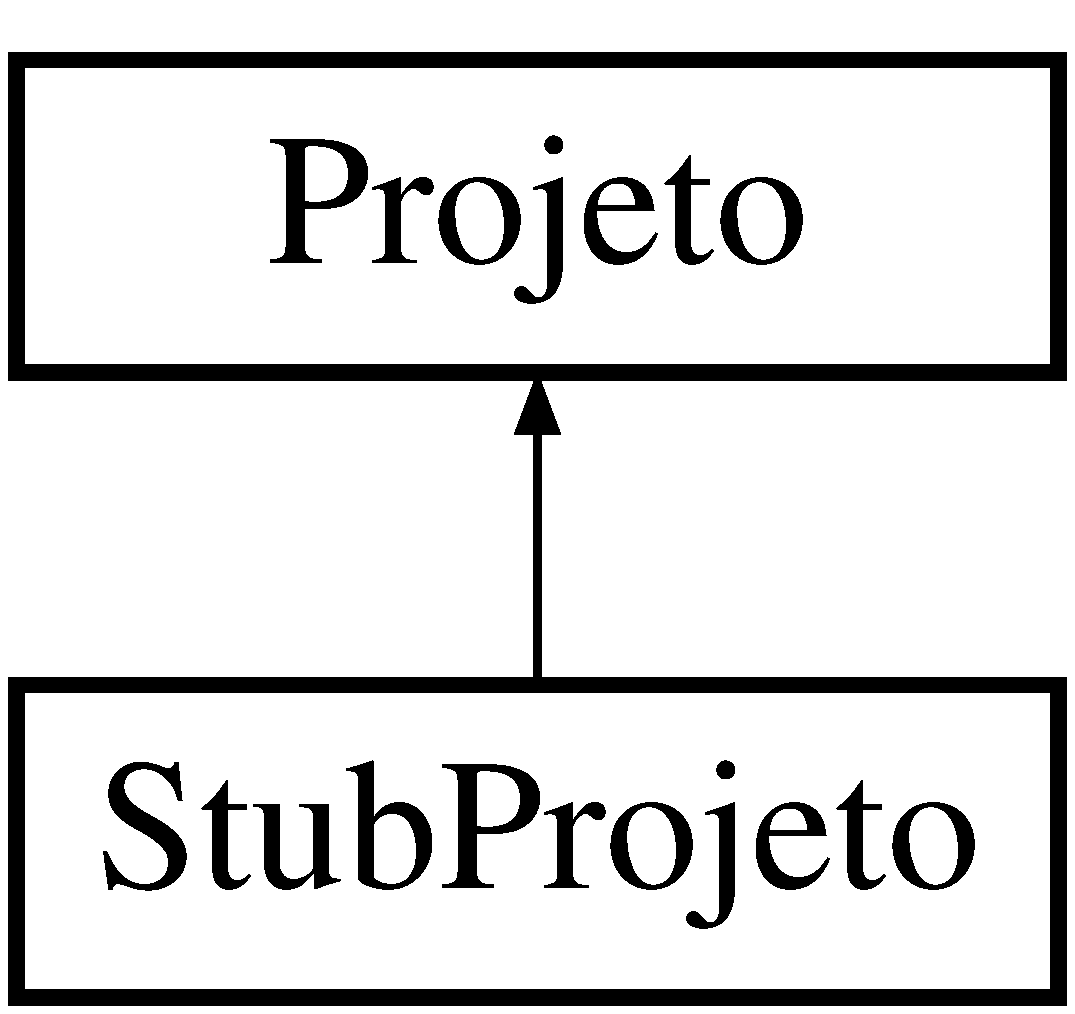
\includegraphics[height=2.000000cm]{class_projeto}
\end{center}
\end{figure}
\subsection*{\-Membros públicos}
\begin{DoxyCompactItemize}
\item 
\hypertarget{class_projeto_ab39919e206b2e33b6ab00bfa3bacd9a5}{
{\bfseries \-Projeto} (\hyperlink{class_matricula}{\-Matricula}, \hyperlink{class_codigo___projeto}{\-Codigo\-\_\-\-Projeto}, \hyperlink{class_data___inicio}{\-Data\-\_\-\-Inicio}, \hyperlink{class_data___termino}{\-Data\-\_\-\-Termino}, \hyperlink{class_nota}{\-Nota})}
\label{class_projeto_ab39919e206b2e33b6ab00bfa3bacd9a5}

\item 
\hyperlink{class_matricula}{\-Matricula} \hyperlink{class_projeto_ab5086bc8a75d77f2065639a836db28c9}{get\-Matricula} () const 
\begin{DoxyCompactList}\small\item\em \-Retorna o valor de \hyperlink{class_matricula}{\-Matricula} da entidade \hyperlink{class_projeto}{\-Projeto}. \end{DoxyCompactList}\item 
void \hyperlink{class_projeto_a2f220b68285d6acefe2b406520326969}{set\-Matricula} (const \hyperlink{class_matricula}{\-Matricula} \&)
\begin{DoxyCompactList}\small\item\em \-Seta o valor de \hyperlink{class_matricula}{\-Matricula} da entidade \hyperlink{class_projeto}{\-Projeto}. \end{DoxyCompactList}\item 
\hyperlink{class_codigo___projeto}{\-Codigo\-\_\-\-Projeto} \hyperlink{class_projeto_a1db1b38d1321c48894e74b7ac679b6e8}{get\-Codigo\-\_\-\-Projeto} () const 
\begin{DoxyCompactList}\small\item\em \-Retorna o valor de \-Codigo de \hyperlink{class_projeto}{\-Projeto} da entidade \hyperlink{class_projeto}{\-Projeto}. \end{DoxyCompactList}\item 
void \hyperlink{class_projeto_aba31c1e58bebad9aa88e4dfc41897bd5}{set\-Codigo\-\_\-\-Projeto} (const \hyperlink{class_codigo___projeto}{\-Codigo\-\_\-\-Projeto} \&)
\begin{DoxyCompactList}\small\item\em \-Seta o valor de \-Codigo de \hyperlink{class_projeto}{\-Projeto} da entidade \hyperlink{class_projeto}{\-Projeto}. \end{DoxyCompactList}\item 
\hyperlink{class_data___inicio}{\-Data\-\_\-\-Inicio} \hyperlink{class_projeto_a309461d7f136b25d6624b054c7beb3f0}{get\-Data\-\_\-\-Inicio} () const 
\begin{DoxyCompactList}\small\item\em \-Retorna o valor de \-Data de \-Inicio da entidade \hyperlink{class_projeto}{\-Projeto}. \end{DoxyCompactList}\item 
void \hyperlink{class_projeto_a699ba726969093cf54a3b1a7677c4434}{set\-Data\-\_\-\-Inicio} (const \hyperlink{class_data___inicio}{\-Data\-\_\-\-Inicio} \&)
\begin{DoxyCompactList}\small\item\em \-Seta o valor de \-Data de \-Inicio da entidade \hyperlink{class_projeto}{\-Projeto}. \end{DoxyCompactList}\item 
\hyperlink{class_data___termino}{\-Data\-\_\-\-Termino} \hyperlink{class_projeto_ae29e37b6730fc277a460d864238df94b}{get\-Data\-\_\-\-Termino} () const 
\begin{DoxyCompactList}\small\item\em \-Retorna o valor de \-Data de \-Termino da entidade \hyperlink{class_projeto}{\-Projeto}. \end{DoxyCompactList}\item 
void \hyperlink{class_projeto_a5371af0d47b30cb46fcd02a4d5fde73f}{set\-Data\-\_\-\-Termino} (const \hyperlink{class_data___termino}{\-Data\-\_\-\-Termino} \&)
\begin{DoxyCompactList}\small\item\em \-Seta o valor de \-Data de \-Termino da entidade \hyperlink{class_projeto}{\-Projeto}. \end{DoxyCompactList}\item 
\hyperlink{class_nota}{\-Nota} \hyperlink{class_projeto_add8f77d42d9c5656456b7625f00c2c02}{get\-Nota} () const 
\begin{DoxyCompactList}\small\item\em \-Retorna o valor de \hyperlink{class_nota}{\-Nota} da entidade \hyperlink{class_projeto}{\-Projeto}. \end{DoxyCompactList}\item 
void \hyperlink{class_projeto_ad074101c3df39dea6c3569c75593f338}{set\-Nota} (const \hyperlink{class_nota}{\-Nota} \&)
\begin{DoxyCompactList}\small\item\em \-Seta o valor de \hyperlink{class_nota}{\-Nota} da entidade \hyperlink{class_projeto}{\-Projeto}. \end{DoxyCompactList}\end{DoxyCompactItemize}


\subsection{\-Descrição detalhada}
\-Classe que representa a entidade \hyperlink{class_projeto}{\-Projeto}. 

\-Contem os atributos que sao instancias das classes \hyperlink{class_matricula}{\-Matricula}, \hyperlink{class_codigo___projeto}{\-Codigo\-\_\-\-Projeto}, \hyperlink{class_data___inicio}{\-Data\-\_\-\-Inicio}, \hyperlink{class_data___termino}{\-Data\-\_\-\-Termino} e \hyperlink{class_nota}{\-Nota} 

\subsection{\-Documentação dos métodos}
\hypertarget{class_projeto_a1db1b38d1321c48894e74b7ac679b6e8}{
\index{\-Projeto@{\-Projeto}!get\-Codigo\-\_\-\-Projeto@{get\-Codigo\-\_\-\-Projeto}}
\index{get\-Codigo\-\_\-\-Projeto@{get\-Codigo\-\_\-\-Projeto}!Projeto@{\-Projeto}}
\subsubsection[{get\-Codigo\-\_\-\-Projeto}]{\setlength{\rightskip}{0pt plus 5cm}{\bf \-Codigo\-\_\-\-Projeto} \-Projeto\-::get\-Codigo\-\_\-\-Projeto (
\begin{DoxyParamCaption}
{}
\end{DoxyParamCaption}
) const\hspace{0.3cm}{\ttfamily  \mbox{[}inline\mbox{]}}}}
\label{class_projeto_a1db1b38d1321c48894e74b7ac679b6e8}


\-Retorna o valor de \-Codigo de \hyperlink{class_projeto}{\-Projeto} da entidade \hyperlink{class_projeto}{\-Projeto}. 

\begin{DoxyReturn}{\-Retorna}
codigo\-\_\-projeto 
\end{DoxyReturn}
\hypertarget{class_projeto_a309461d7f136b25d6624b054c7beb3f0}{
\index{\-Projeto@{\-Projeto}!get\-Data\-\_\-\-Inicio@{get\-Data\-\_\-\-Inicio}}
\index{get\-Data\-\_\-\-Inicio@{get\-Data\-\_\-\-Inicio}!Projeto@{\-Projeto}}
\subsubsection[{get\-Data\-\_\-\-Inicio}]{\setlength{\rightskip}{0pt plus 5cm}{\bf \-Data\-\_\-\-Inicio} \-Projeto\-::get\-Data\-\_\-\-Inicio (
\begin{DoxyParamCaption}
{}
\end{DoxyParamCaption}
) const\hspace{0.3cm}{\ttfamily  \mbox{[}inline\mbox{]}}}}
\label{class_projeto_a309461d7f136b25d6624b054c7beb3f0}


\-Retorna o valor de \-Data de \-Inicio da entidade \hyperlink{class_projeto}{\-Projeto}. 

\begin{DoxyReturn}{\-Retorna}
data\-\_\-inicio 
\end{DoxyReturn}
\hypertarget{class_projeto_ae29e37b6730fc277a460d864238df94b}{
\index{\-Projeto@{\-Projeto}!get\-Data\-\_\-\-Termino@{get\-Data\-\_\-\-Termino}}
\index{get\-Data\-\_\-\-Termino@{get\-Data\-\_\-\-Termino}!Projeto@{\-Projeto}}
\subsubsection[{get\-Data\-\_\-\-Termino}]{\setlength{\rightskip}{0pt plus 5cm}{\bf \-Data\-\_\-\-Termino} \-Projeto\-::get\-Data\-\_\-\-Termino (
\begin{DoxyParamCaption}
{}
\end{DoxyParamCaption}
) const\hspace{0.3cm}{\ttfamily  \mbox{[}inline\mbox{]}}}}
\label{class_projeto_ae29e37b6730fc277a460d864238df94b}


\-Retorna o valor de \-Data de \-Termino da entidade \hyperlink{class_projeto}{\-Projeto}. 

\begin{DoxyReturn}{\-Retorna}
data\-\_\-termino 
\end{DoxyReturn}
\hypertarget{class_projeto_ab5086bc8a75d77f2065639a836db28c9}{
\index{\-Projeto@{\-Projeto}!get\-Matricula@{get\-Matricula}}
\index{get\-Matricula@{get\-Matricula}!Projeto@{\-Projeto}}
\subsubsection[{get\-Matricula}]{\setlength{\rightskip}{0pt plus 5cm}{\bf \-Matricula} \-Projeto\-::get\-Matricula (
\begin{DoxyParamCaption}
{}
\end{DoxyParamCaption}
) const\hspace{0.3cm}{\ttfamily  \mbox{[}inline\mbox{]}}}}
\label{class_projeto_ab5086bc8a75d77f2065639a836db28c9}


\-Retorna o valor de \hyperlink{class_matricula}{\-Matricula} da entidade \hyperlink{class_projeto}{\-Projeto}. 

\begin{DoxyReturn}{\-Retorna}
matricula 
\end{DoxyReturn}
\hypertarget{class_projeto_add8f77d42d9c5656456b7625f00c2c02}{
\index{\-Projeto@{\-Projeto}!get\-Nota@{get\-Nota}}
\index{get\-Nota@{get\-Nota}!Projeto@{\-Projeto}}
\subsubsection[{get\-Nota}]{\setlength{\rightskip}{0pt plus 5cm}{\bf \-Nota} \-Projeto\-::get\-Nota (
\begin{DoxyParamCaption}
{}
\end{DoxyParamCaption}
) const\hspace{0.3cm}{\ttfamily  \mbox{[}inline\mbox{]}}}}
\label{class_projeto_add8f77d42d9c5656456b7625f00c2c02}


\-Retorna o valor de \hyperlink{class_nota}{\-Nota} da entidade \hyperlink{class_projeto}{\-Projeto}. 

\begin{DoxyReturn}{\-Retorna}
nota 
\end{DoxyReturn}
\hypertarget{class_projeto_aba31c1e58bebad9aa88e4dfc41897bd5}{
\index{\-Projeto@{\-Projeto}!set\-Codigo\-\_\-\-Projeto@{set\-Codigo\-\_\-\-Projeto}}
\index{set\-Codigo\-\_\-\-Projeto@{set\-Codigo\-\_\-\-Projeto}!Projeto@{\-Projeto}}
\subsubsection[{set\-Codigo\-\_\-\-Projeto}]{\setlength{\rightskip}{0pt plus 5cm}void \-Projeto\-::set\-Codigo\-\_\-\-Projeto (
\begin{DoxyParamCaption}
\item[{const {\bf \-Codigo\-\_\-\-Projeto} \&}]{}
\end{DoxyParamCaption}
)}}
\label{class_projeto_aba31c1e58bebad9aa88e4dfc41897bd5}


\-Seta o valor de \-Codigo de \hyperlink{class_projeto}{\-Projeto} da entidade \hyperlink{class_projeto}{\-Projeto}. 


\begin{DoxyParams}{\-Parâmetros}
{\em \-Codigo\-\_\-\-Projeto\&} & \\
\hline
\end{DoxyParams}
\hypertarget{class_projeto_a699ba726969093cf54a3b1a7677c4434}{
\index{\-Projeto@{\-Projeto}!set\-Data\-\_\-\-Inicio@{set\-Data\-\_\-\-Inicio}}
\index{set\-Data\-\_\-\-Inicio@{set\-Data\-\_\-\-Inicio}!Projeto@{\-Projeto}}
\subsubsection[{set\-Data\-\_\-\-Inicio}]{\setlength{\rightskip}{0pt plus 5cm}void \-Projeto\-::set\-Data\-\_\-\-Inicio (
\begin{DoxyParamCaption}
\item[{const {\bf \-Data\-\_\-\-Inicio} \&}]{}
\end{DoxyParamCaption}
)}}
\label{class_projeto_a699ba726969093cf54a3b1a7677c4434}


\-Seta o valor de \-Data de \-Inicio da entidade \hyperlink{class_projeto}{\-Projeto}. 


\begin{DoxyParams}{\-Parâmetros}
{\em \-Data\-\_\-\-Inicio\&} & \\
\hline
\end{DoxyParams}
\hypertarget{class_projeto_a5371af0d47b30cb46fcd02a4d5fde73f}{
\index{\-Projeto@{\-Projeto}!set\-Data\-\_\-\-Termino@{set\-Data\-\_\-\-Termino}}
\index{set\-Data\-\_\-\-Termino@{set\-Data\-\_\-\-Termino}!Projeto@{\-Projeto}}
\subsubsection[{set\-Data\-\_\-\-Termino}]{\setlength{\rightskip}{0pt plus 5cm}void \-Projeto\-::set\-Data\-\_\-\-Termino (
\begin{DoxyParamCaption}
\item[{const {\bf \-Data\-\_\-\-Termino} \&}]{}
\end{DoxyParamCaption}
)}}
\label{class_projeto_a5371af0d47b30cb46fcd02a4d5fde73f}


\-Seta o valor de \-Data de \-Termino da entidade \hyperlink{class_projeto}{\-Projeto}. 


\begin{DoxyParams}{\-Parâmetros}
{\em \-Data\-\_\-\-Termino\&} & \\
\hline
\end{DoxyParams}
\hypertarget{class_projeto_a2f220b68285d6acefe2b406520326969}{
\index{\-Projeto@{\-Projeto}!set\-Matricula@{set\-Matricula}}
\index{set\-Matricula@{set\-Matricula}!Projeto@{\-Projeto}}
\subsubsection[{set\-Matricula}]{\setlength{\rightskip}{0pt plus 5cm}void \-Projeto\-::set\-Matricula (
\begin{DoxyParamCaption}
\item[{const {\bf \-Matricula} \&}]{}
\end{DoxyParamCaption}
)}}
\label{class_projeto_a2f220b68285d6acefe2b406520326969}


\-Seta o valor de \hyperlink{class_matricula}{\-Matricula} da entidade \hyperlink{class_projeto}{\-Projeto}. 


\begin{DoxyParams}{\-Parâmetros}
{\em \-Matricula\&} & \\
\hline
\end{DoxyParams}
\hypertarget{class_projeto_ad074101c3df39dea6c3569c75593f338}{
\index{\-Projeto@{\-Projeto}!set\-Nota@{set\-Nota}}
\index{set\-Nota@{set\-Nota}!Projeto@{\-Projeto}}
\subsubsection[{set\-Nota}]{\setlength{\rightskip}{0pt plus 5cm}void \-Projeto\-::set\-Nota (
\begin{DoxyParamCaption}
\item[{const {\bf \-Nota} \&}]{}
\end{DoxyParamCaption}
)}}
\label{class_projeto_ad074101c3df39dea6c3569c75593f338}


\-Seta o valor de \hyperlink{class_nota}{\-Nota} da entidade \hyperlink{class_projeto}{\-Projeto}. 


\begin{DoxyParams}{\-Parâmetros}
{\em \-Nota\&} & \\
\hline
\end{DoxyParams}


\-A documentação para esta classe foi gerada a partir do seguinte ficheiro\-:\begin{DoxyCompactItemize}
\item 
\-Entidades.\-h\end{DoxyCompactItemize}

\hypertarget{class_protocolo_fase}{
\section{\-Referência à classe \-Protocolo\-Fase}
\label{class_protocolo_fase}\index{\-Protocolo\-Fase@{\-Protocolo\-Fase}}
}


\-Classe abstrata que faz a ligacao entre camada de interacao do usuario e logica de negocio.  




{\ttfamily \#include $<$\-Protocolos.\-h$>$}

\-Diagrama de heranças da classe \-Protocolo\-Fase\begin{figure}[H]
\begin{center}
\leavevmode
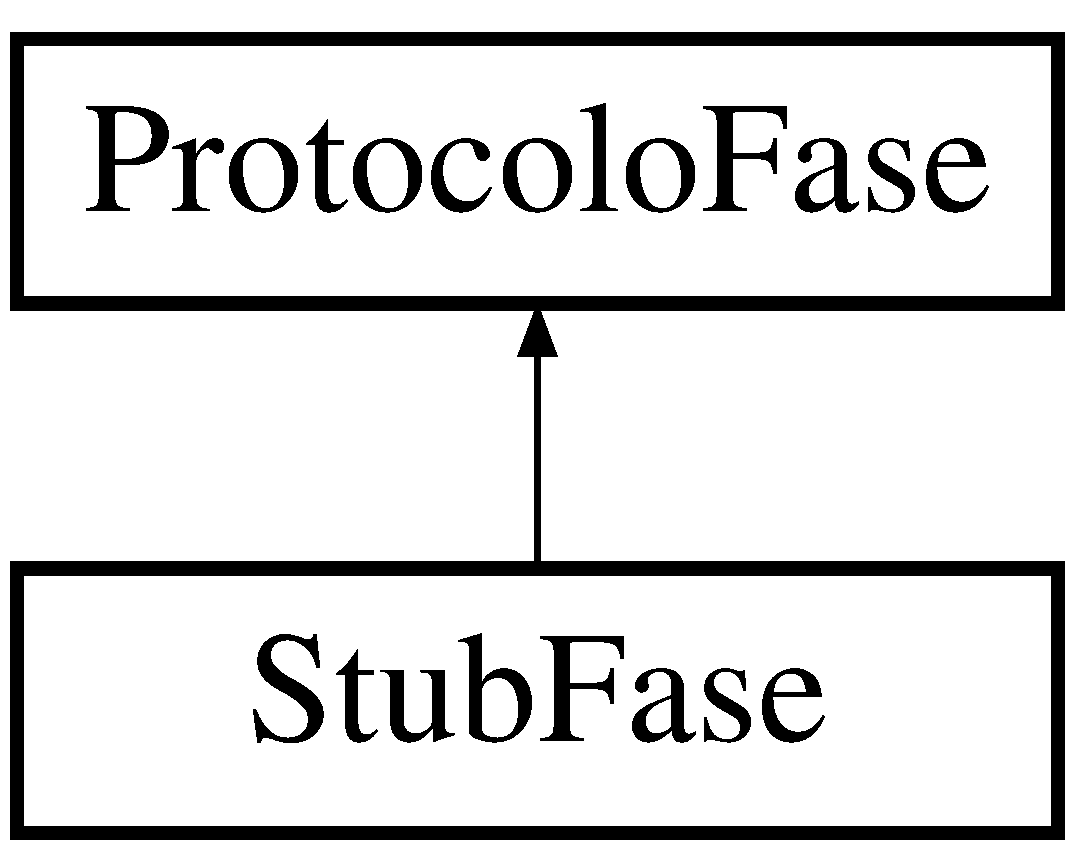
\includegraphics[height=2.000000cm]{class_protocolo_fase}
\end{center}
\end{figure}
\subsection*{\-Membros públicos}
\begin{DoxyCompactItemize}
\item 
\hypertarget{class_protocolo_fase_aac28718e85013963a84bb2ba5388e33f}{
virtual void {\bfseries cadastrar} (\hyperlink{class_fase}{\-Fase})=0}
\label{class_protocolo_fase_aac28718e85013963a84bb2ba5388e33f}

\item 
\hypertarget{class_protocolo_fase_a6237c5adc12aa6e5e5b2326b46d09b23}{
virtual void {\bfseries atualizar} (\hyperlink{class_fase}{\-Fase})=0}
\label{class_protocolo_fase_a6237c5adc12aa6e5e5b2326b46d09b23}

\item 
\hypertarget{class_protocolo_fase_ac062b94f702308fb107af10004ff8b6f}{
virtual void {\bfseries set\-Persistencia} (\hyperlink{class_protocolo_persistencia}{\-Protocolo\-Persistencia} $\ast$)=0}
\label{class_protocolo_fase_ac062b94f702308fb107af10004ff8b6f}

\end{DoxyCompactItemize}


\subsection{\-Descrição detalhada}
\-Classe abstrata que faz a ligacao entre camada de interacao do usuario e logica de negocio. 

\-Manda os servicos de cadastrar e atualizar \hyperlink{class_fase}{\-Fase} e encaminha para a logica de negocio 

\-A documentação para esta classe foi gerada a partir do seguinte ficheiro\-:\begin{DoxyCompactItemize}
\item 
\-Protocolos.\-h\end{DoxyCompactItemize}

\hypertarget{class_protocolo_int}{
\section{\-Referência à classe \-Protocolo\-Int}
\label{class_protocolo_int}\index{\-Protocolo\-Int@{\-Protocolo\-Int}}
}


\-Classe abstrata que e utilizada para a escolha das \-Controladoras de \-Interacao, atraves dos protocolos especificos.  




{\ttfamily \#include $<$\-Protocolos.\-h$>$}

\-Diagrama de heranças da classe \-Protocolo\-Int\begin{figure}[H]
\begin{center}
\leavevmode
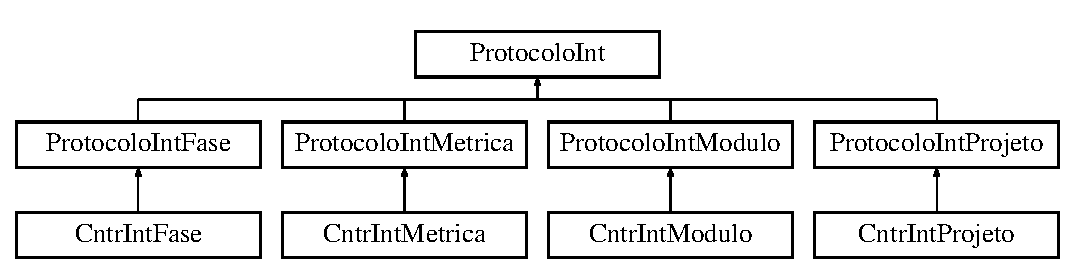
\includegraphics[height=3.000000cm]{class_protocolo_int}
\end{center}
\end{figure}
\subsection*{\-Membros públicos}
\begin{DoxyCompactItemize}
\item 
\hypertarget{class_protocolo_int_a3e0dfb20671385070149211a28a19f85}{
virtual void {\bfseries executar} ()=0}
\label{class_protocolo_int_a3e0dfb20671385070149211a28a19f85}

\end{DoxyCompactItemize}


\subsection{\-Descrição detalhada}
\-Classe abstrata que e utilizada para a escolha das \-Controladoras de \-Interacao, atraves dos protocolos especificos. 

\-A documentação para esta classe foi gerada a partir do seguinte ficheiro\-:\begin{DoxyCompactItemize}
\item 
\-Protocolos.\-h\end{DoxyCompactItemize}

\hypertarget{class_protocolo_int_fase}{
\section{\-Referência à classe \-Protocolo\-Int\-Fase}
\label{class_protocolo_int_fase}\index{\-Protocolo\-Int\-Fase@{\-Protocolo\-Int\-Fase}}
}


\-Classe abstrata que seleciona a \-Controladora de \hyperlink{class_fase}{\-Fase}.  




{\ttfamily \#include $<$\-Protocolos.\-h$>$}

\-Diagrama de heranças da classe \-Protocolo\-Int\-Fase\begin{figure}[H]
\begin{center}
\leavevmode
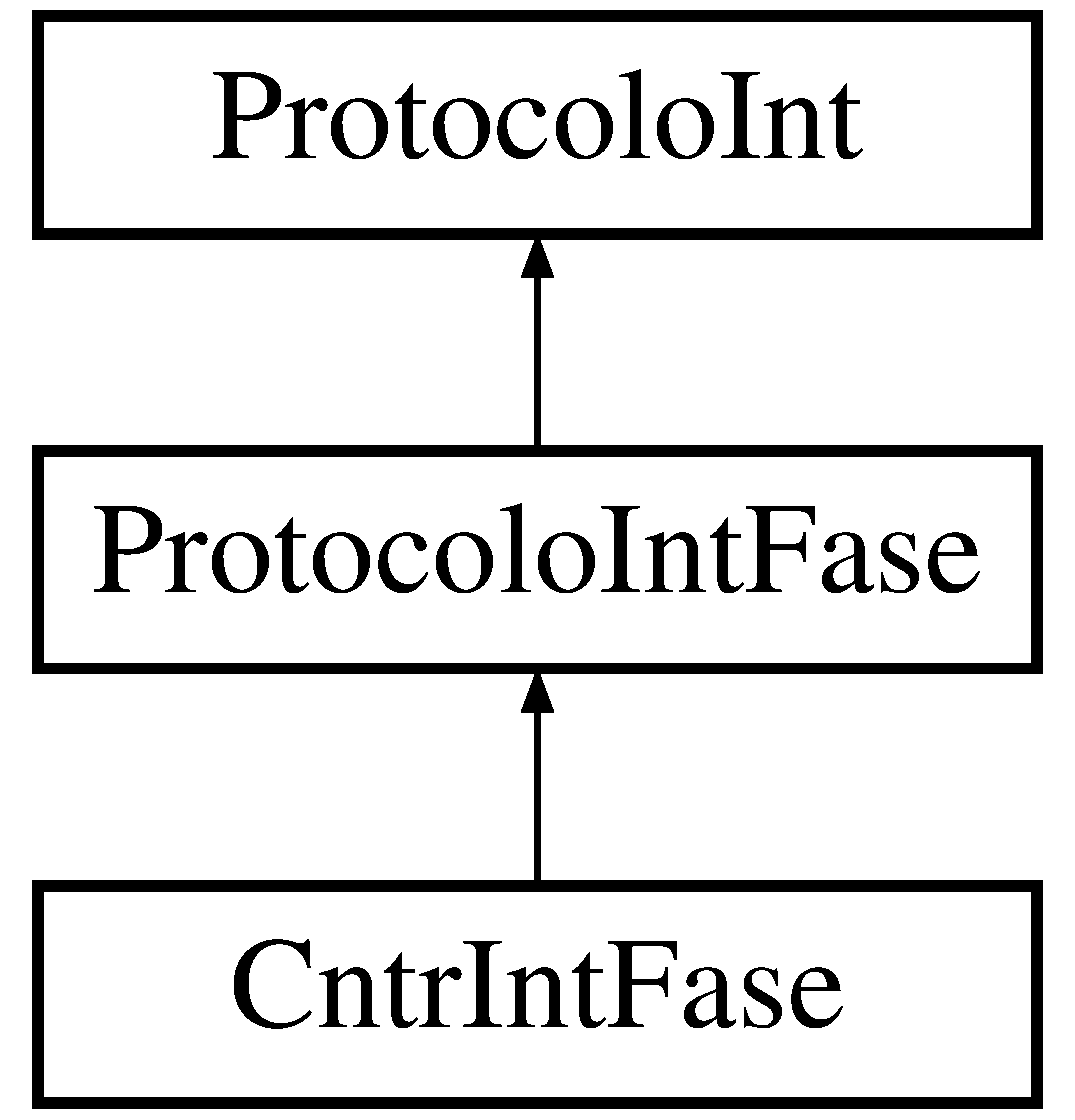
\includegraphics[height=3.000000cm]{class_protocolo_int_fase}
\end{center}
\end{figure}
\subsection*{\-Membros públicos}
\begin{DoxyCompactItemize}
\item 
\hypertarget{class_protocolo_int_fase_a3895ab786d72b5294f8f3b64f0c607dc}{
virtual void {\bfseries set\-Cntr} (\hyperlink{class_protocolo_fase}{\-Protocolo\-Fase} $\ast$)=0}
\label{class_protocolo_int_fase_a3895ab786d72b5294f8f3b64f0c607dc}

\end{DoxyCompactItemize}


\subsection{\-Descrição detalhada}
\-Classe abstrata que seleciona a \-Controladora de \hyperlink{class_fase}{\-Fase}. 

\-Herda os servicos da classe \hyperlink{class_protocolo_int}{\-Protocolo\-Int} e seleciona a \-Controladora de \hyperlink{class_fase}{\-Fase} 

\-A documentação para esta classe foi gerada a partir do seguinte ficheiro\-:\begin{DoxyCompactItemize}
\item 
\-Protocolos.\-h\end{DoxyCompactItemize}

\hypertarget{class_protocolo_int_metrica}{
\section{\-Referência à classe \-Protocolo\-Int\-Metrica}
\label{class_protocolo_int_metrica}\index{\-Protocolo\-Int\-Metrica@{\-Protocolo\-Int\-Metrica}}
}


\-Classe abstrata que seleciona a \-Controladora de \hyperlink{class_metrica}{\-Metrica}.  




{\ttfamily \#include $<$\-Protocolos.\-h$>$}

\-Diagrama de heranças da classe \-Protocolo\-Int\-Metrica\begin{figure}[H]
\begin{center}
\leavevmode
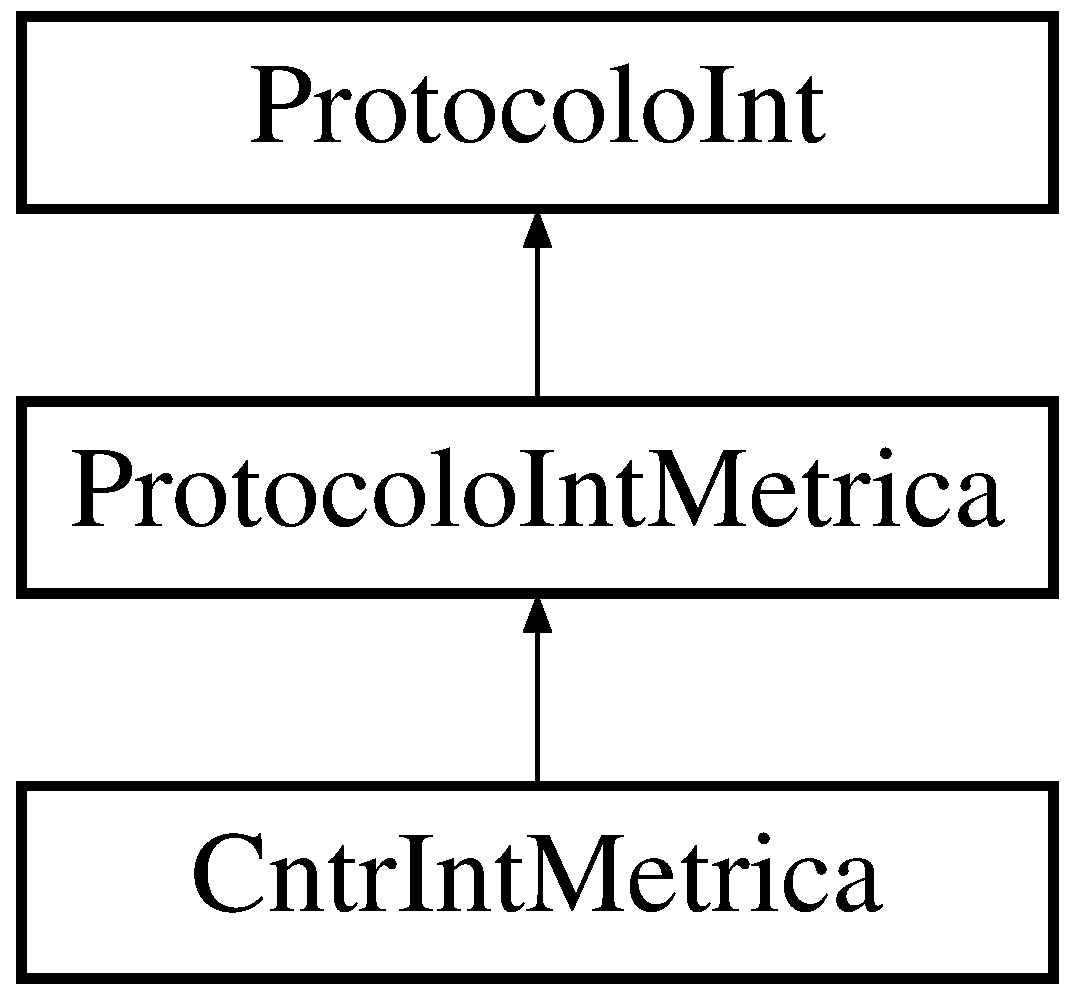
\includegraphics[height=3.000000cm]{class_protocolo_int_metrica}
\end{center}
\end{figure}
\subsection*{\-Membros públicos}
\begin{DoxyCompactItemize}
\item 
\hypertarget{class_protocolo_int_metrica_a554fb5978dea8a6551ef59ccc18024a8}{
virtual void {\bfseries set\-Cntr} (\hyperlink{class_protocolo_metrica}{\-Protocolo\-Metrica} $\ast$)=0}
\label{class_protocolo_int_metrica_a554fb5978dea8a6551ef59ccc18024a8}

\end{DoxyCompactItemize}


\subsection{\-Descrição detalhada}
\-Classe abstrata que seleciona a \-Controladora de \hyperlink{class_metrica}{\-Metrica}. 

\-Herda os servicos da classe \hyperlink{class_protocolo_int}{\-Protocolo\-Int} e seleciona a \-Controladora de \hyperlink{class_metrica}{\-Metrica} 

\-A documentação para esta classe foi gerada a partir do seguinte ficheiro\-:\begin{DoxyCompactItemize}
\item 
\-Protocolos.\-h\end{DoxyCompactItemize}

\hypertarget{class_protocolo_int_modulo}{
\section{\-Referência à classe \-Protocolo\-Int\-Modulo}
\label{class_protocolo_int_modulo}\index{\-Protocolo\-Int\-Modulo@{\-Protocolo\-Int\-Modulo}}
}


\-Classe abstrata que seleciona a \-Controladora de \hyperlink{class_modulo}{\-Modulo}.  




{\ttfamily \#include $<$\-Protocolos.\-h$>$}

\-Diagrama de heranças da classe \-Protocolo\-Int\-Modulo\begin{figure}[H]
\begin{center}
\leavevmode
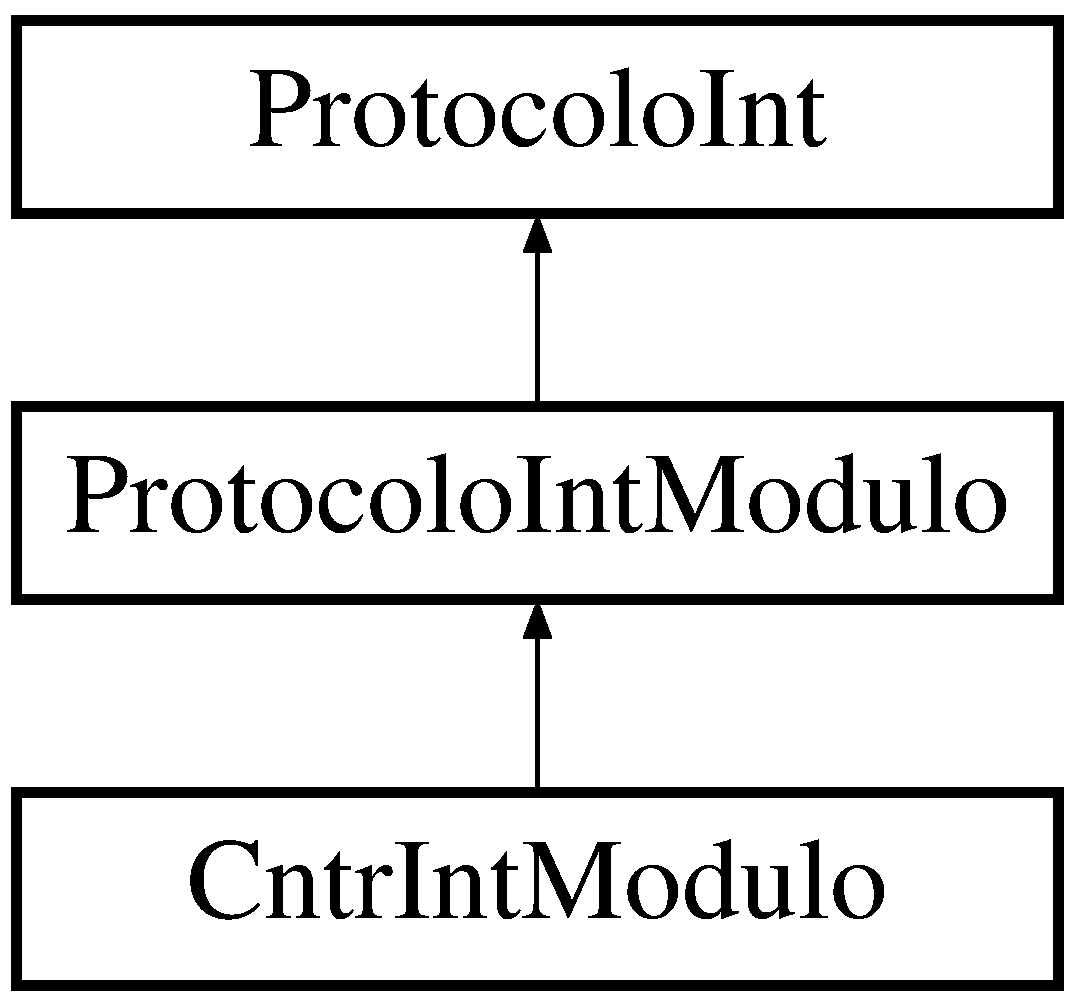
\includegraphics[height=3.000000cm]{class_protocolo_int_modulo}
\end{center}
\end{figure}
\subsection*{\-Membros públicos}
\begin{DoxyCompactItemize}
\item 
\hypertarget{class_protocolo_int_modulo_a493ea7b6822cac39cd5ae8e31af6fb39}{
virtual void {\bfseries set\-Cntr} (\hyperlink{class_protocolo_modulo}{\-Protocolo\-Modulo} $\ast$)=0}
\label{class_protocolo_int_modulo_a493ea7b6822cac39cd5ae8e31af6fb39}

\end{DoxyCompactItemize}


\subsection{\-Descrição detalhada}
\-Classe abstrata que seleciona a \-Controladora de \hyperlink{class_modulo}{\-Modulo}. 

\-Herda os servicos da classe \hyperlink{class_protocolo_int}{\-Protocolo\-Int} e seleciona a \-Controladora de \hyperlink{class_modulo}{\-Modulo} 

\-A documentação para esta classe foi gerada a partir do seguinte ficheiro\-:\begin{DoxyCompactItemize}
\item 
\-Protocolos.\-h\end{DoxyCompactItemize}

\hypertarget{class_protocolo_int_projeto}{
\section{\-Referência à classe \-Protocolo\-Int\-Projeto}
\label{class_protocolo_int_projeto}\index{\-Protocolo\-Int\-Projeto@{\-Protocolo\-Int\-Projeto}}
}


\-Classe abstrata que seleciona a \-Controladora de \hyperlink{class_projeto}{\-Projeto}.  




{\ttfamily \#include $<$\-Protocolos.\-h$>$}

\-Diagrama de heranças da classe \-Protocolo\-Int\-Projeto\begin{figure}[H]
\begin{center}
\leavevmode
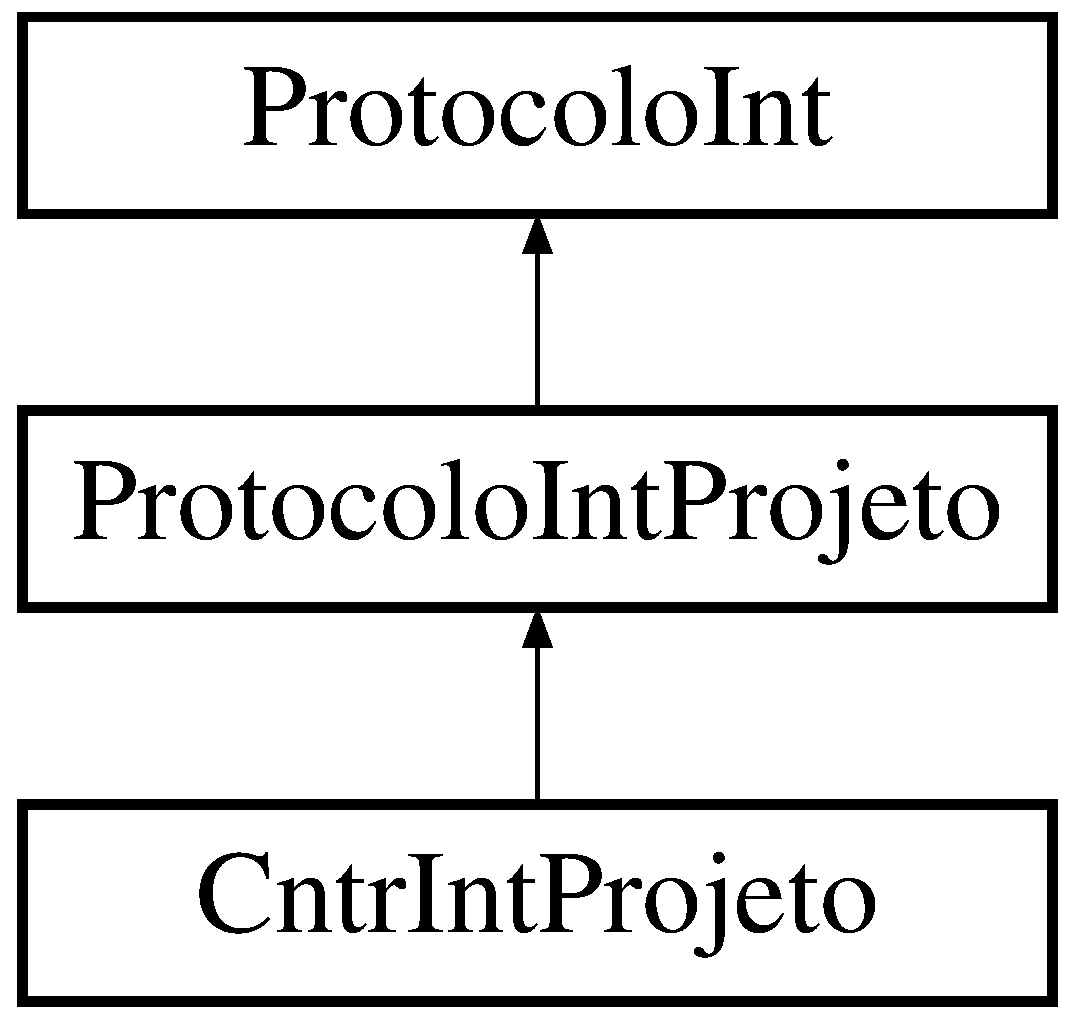
\includegraphics[height=3.000000cm]{class_protocolo_int_projeto}
\end{center}
\end{figure}
\subsection*{\-Membros públicos}
\begin{DoxyCompactItemize}
\item 
\hypertarget{class_protocolo_int_projeto_a4d71d138aa99b9ce9deb055fee8f4338}{
virtual void {\bfseries set\-Cntr} (\hyperlink{class_protocolo_projeto}{\-Protocolo\-Projeto} $\ast$)=0}
\label{class_protocolo_int_projeto_a4d71d138aa99b9ce9deb055fee8f4338}

\end{DoxyCompactItemize}


\subsection{\-Descrição detalhada}
\-Classe abstrata que seleciona a \-Controladora de \hyperlink{class_projeto}{\-Projeto}. 

\-Herda os servicos da classe \hyperlink{class_protocolo_int}{\-Protocolo\-Int} e seleciona a \-Controladora de \hyperlink{class_projeto}{\-Projeto} 

\-A documentação para esta classe foi gerada a partir do seguinte ficheiro\-:\begin{DoxyCompactItemize}
\item 
\-Protocolos.\-h\end{DoxyCompactItemize}

\hypertarget{class_protocolo_metrica}{
\section{\-Referência à classe \-Protocolo\-Metrica}
\label{class_protocolo_metrica}\index{\-Protocolo\-Metrica@{\-Protocolo\-Metrica}}
}


\-Classe abstrata que faz a ligacao entre interacao do usuario e logica de negocio.  




{\ttfamily \#include $<$\-Protocolos.\-h$>$}

\-Diagrama de heranças da classe \-Protocolo\-Metrica\begin{figure}[H]
\begin{center}
\leavevmode
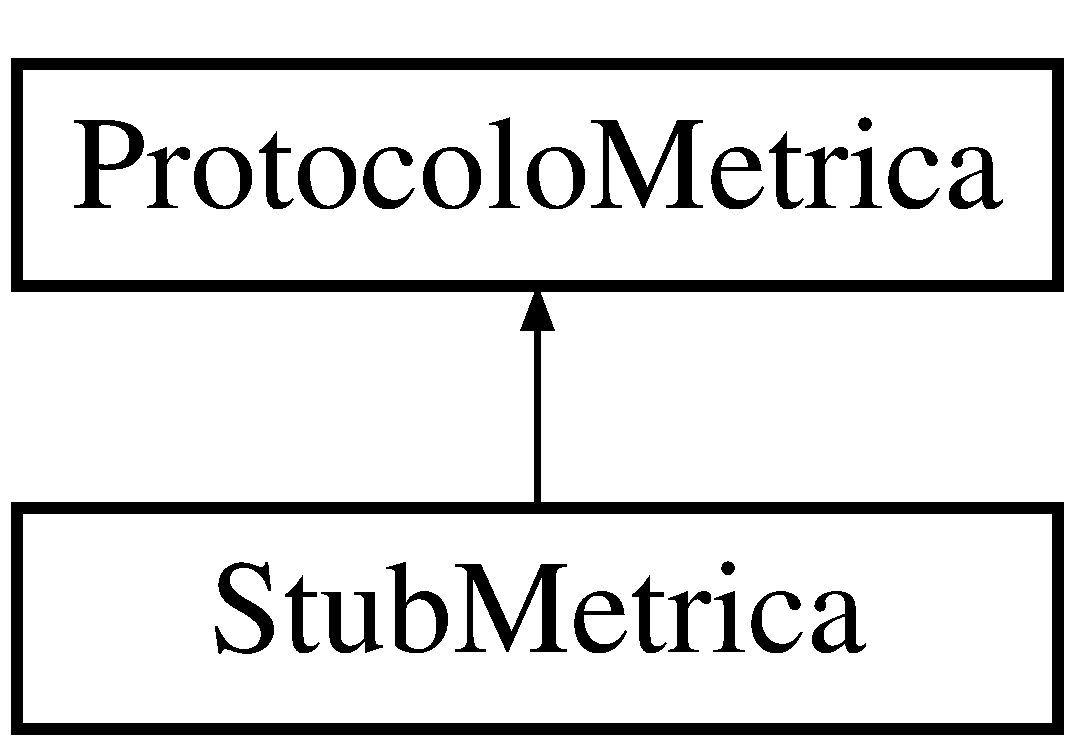
\includegraphics[height=2.000000cm]{class_protocolo_metrica}
\end{center}
\end{figure}
\subsection*{\-Membros públicos}
\begin{DoxyCompactItemize}
\item 
\hypertarget{class_protocolo_metrica_a25f884c5349e9791d8f482c70e5758e5}{
virtual void {\bfseries numero\-\_\-linhas} (\hyperlink{class_metrica}{\-Metrica})=0}
\label{class_protocolo_metrica_a25f884c5349e9791d8f482c70e5758e5}

\item 
\hypertarget{class_protocolo_metrica_ac79ddc9645f304b502beb9bcac0c02d4}{
virtual void {\bfseries tempo\-\_\-gasto\-\_\-projeto} (\hyperlink{class_metrica}{\-Metrica})=0}
\label{class_protocolo_metrica_ac79ddc9645f304b502beb9bcac0c02d4}

\item 
\hypertarget{class_protocolo_metrica_ace1e8a26124c509054786c482cfecb8b}{
virtual void {\bfseries tempo\-\_\-gasto\-\_\-modulo} (\hyperlink{class_metrica}{\-Metrica})=0}
\label{class_protocolo_metrica_ace1e8a26124c509054786c482cfecb8b}

\item 
\hypertarget{class_protocolo_metrica_a1180e2c970d5e853d125e30c77fe1f0e}{
virtual void {\bfseries produtividade\-\_\-projeto} (\hyperlink{class_metrica}{\-Metrica})=0}
\label{class_protocolo_metrica_a1180e2c970d5e853d125e30c77fe1f0e}

\item 
\hypertarget{class_protocolo_metrica_a430351b35ef34d8ae90ea4d517af20be}{
virtual void {\bfseries produtividade\-\_\-modulo} (\hyperlink{class_metrica}{\-Metrica})=0}
\label{class_protocolo_metrica_a430351b35ef34d8ae90ea4d517af20be}

\item 
\hypertarget{class_protocolo_metrica_ab9cd9abb8cf1d6fcc65e271547267e9e}{
virtual void {\bfseries nota} (\hyperlink{class_metrica}{\-Metrica})=0}
\label{class_protocolo_metrica_ab9cd9abb8cf1d6fcc65e271547267e9e}

\item 
\hypertarget{class_protocolo_metrica_a27ce5bf3ade36e0af9624b5b59043eb2}{
virtual void {\bfseries tamanho\-\_\-medio} (\hyperlink{class_metrica}{\-Metrica})=0}
\label{class_protocolo_metrica_a27ce5bf3ade36e0af9624b5b59043eb2}

\item 
\hypertarget{class_protocolo_metrica_a6125a4e8a938b95f39e7901bd1e2a275}{
virtual void {\bfseries produtividade\-\_\-media} (\hyperlink{class_metrica}{\-Metrica})=0}
\label{class_protocolo_metrica_a6125a4e8a938b95f39e7901bd1e2a275}

\item 
\hypertarget{class_protocolo_metrica_a8d46750f979501d8e5b8e21a2eae09bb}{
virtual void {\bfseries set\-Persistencia} (\hyperlink{class_protocolo_persistencia}{\-Protocolo\-Persistencia} $\ast$)=0}
\label{class_protocolo_metrica_a8d46750f979501d8e5b8e21a2eae09bb}

\end{DoxyCompactItemize}


\subsection{\-Descrição detalhada}
\-Classe abstrata que faz a ligacao entre interacao do usuario e logica de negocio. 

\-Manda os servicos de calcular numero de linhas, tempo gasto no projeto e tempo gasto no modulo, a produtividade do projeto e do modulo, nota, o tamanho medio e a produtividade medio da \hyperlink{class_metrica}{\-Metrica} encaminha para a logica de negocio 

\-A documentação para esta classe foi gerada a partir do seguinte ficheiro\-:\begin{DoxyCompactItemize}
\item 
\-Protocolos.\-h\end{DoxyCompactItemize}

\hypertarget{class_protocolo_modulo}{
\section{\-Referência à classe \-Protocolo\-Modulo}
\label{class_protocolo_modulo}\index{\-Protocolo\-Modulo@{\-Protocolo\-Modulo}}
}


\-Classe abstrata que faz a ligacao entre interacao do usuario e logica de negocio.  




{\ttfamily \#include $<$\-Protocolos.\-h$>$}

\-Diagrama de heranças da classe \-Protocolo\-Modulo\begin{figure}[H]
\begin{center}
\leavevmode
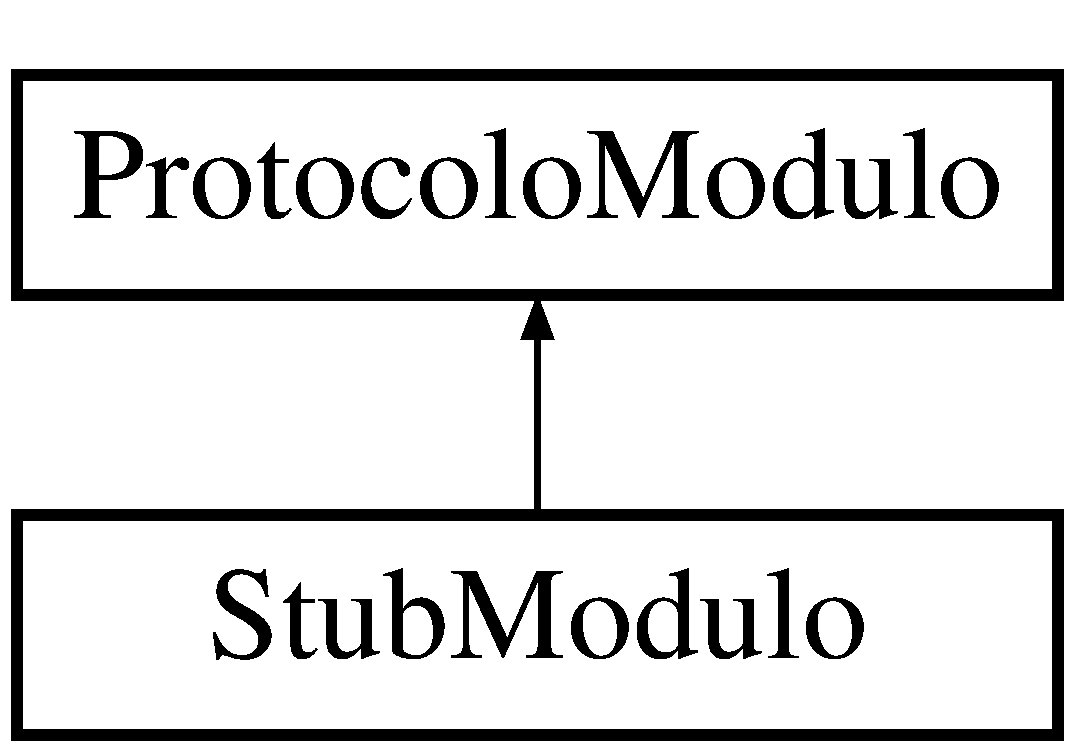
\includegraphics[height=2.000000cm]{class_protocolo_modulo}
\end{center}
\end{figure}
\subsection*{\-Membros públicos}
\begin{DoxyCompactItemize}
\item 
\hypertarget{class_protocolo_modulo_a806c451fa3191899a1485fc8b1384ea1}{
virtual void {\bfseries cadastrar} (const \hyperlink{class_modulo}{\-Modulo} \&)=0}
\label{class_protocolo_modulo_a806c451fa3191899a1485fc8b1384ea1}

\item 
\hypertarget{class_protocolo_modulo_ad7d56410221ef77347232fa254a0ec03}{
virtual void {\bfseries remover} (\hyperlink{class_codigo___modulo}{\-Codigo\-\_\-\-Modulo})=0}
\label{class_protocolo_modulo_ad7d56410221ef77347232fa254a0ec03}

\item 
\hypertarget{class_protocolo_modulo_ac8dc9878f6d12787b423cd18b7f71ef9}{
virtual \hyperlink{class_modulo}{\-Modulo} {\bfseries pesquisar} (\hyperlink{class_codigo___modulo}{\-Codigo\-\_\-\-Modulo})=0}
\label{class_protocolo_modulo_ac8dc9878f6d12787b423cd18b7f71ef9}

\item 
\hypertarget{class_protocolo_modulo_afe596d0942c2db35a16250521a17f1c9}{
virtual void {\bfseries atualizar} (\hyperlink{class_modulo}{\-Modulo} $\ast$)=0}
\label{class_protocolo_modulo_afe596d0942c2db35a16250521a17f1c9}

\item 
\hypertarget{class_protocolo_modulo_aa64f43a4b1f736fde6ca1bd2dfe9ec59}{
virtual void {\bfseries set\-Persistencia} (\hyperlink{class_protocolo_persistencia}{\-Protocolo\-Persistencia} $\ast$)=0}
\label{class_protocolo_modulo_aa64f43a4b1f736fde6ca1bd2dfe9ec59}

\end{DoxyCompactItemize}


\subsection{\-Descrição detalhada}
\-Classe abstrata que faz a ligacao entre interacao do usuario e logica de negocio. 

\-Manda os servicos de cadastrar, remover, pesquisar e atualizar \hyperlink{class_modulo}{\-Modulo} e encaminha para a logica de negocio 

\-A documentação para esta classe foi gerada a partir do seguinte ficheiro\-:\begin{DoxyCompactItemize}
\item 
\-Protocolos.\-h\end{DoxyCompactItemize}

\hypertarget{class_protocolo_projeto}{
\section{\-Referência à classe \-Protocolo\-Projeto}
\label{class_protocolo_projeto}\index{\-Protocolo\-Projeto@{\-Protocolo\-Projeto}}
}


\-Classe abstrata que faz a ligacao entre interacao do usuario e logica de negocio.  




{\ttfamily \#include $<$\-Protocolos.\-h$>$}

\-Diagrama de heranças da classe \-Protocolo\-Projeto\begin{figure}[H]
\begin{center}
\leavevmode
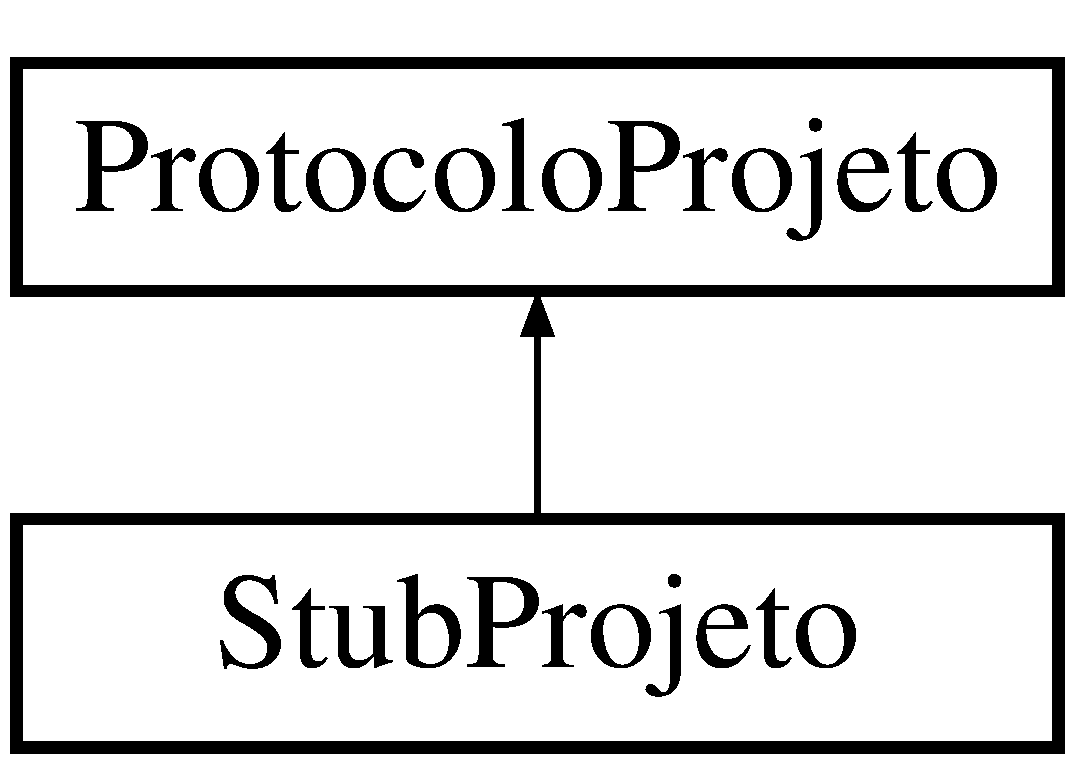
\includegraphics[height=2.000000cm]{class_protocolo_projeto}
\end{center}
\end{figure}
\subsection*{\-Membros públicos}
\begin{DoxyCompactItemize}
\item 
\hypertarget{class_protocolo_projeto_a9f40bae886ad64945119c11e84b2f0d5}{
virtual void {\bfseries cadastrar} (const \hyperlink{class_projeto}{\-Projeto} \&)=0}
\label{class_protocolo_projeto_a9f40bae886ad64945119c11e84b2f0d5}

\item 
\hypertarget{class_protocolo_projeto_a083c4caec4591d509e141e97d698aa2d}{
virtual void {\bfseries remover} (\hyperlink{class_codigo___projeto}{\-Codigo\-\_\-\-Projeto})=0}
\label{class_protocolo_projeto_a083c4caec4591d509e141e97d698aa2d}

\item 
\hypertarget{class_protocolo_projeto_a01c7c0f083c533c197b7c4e69f56ed59}{
virtual \hyperlink{class_projeto}{\-Projeto} {\bfseries pesquisar} (\hyperlink{class_codigo___projeto}{\-Codigo\-\_\-\-Projeto})=0}
\label{class_protocolo_projeto_a01c7c0f083c533c197b7c4e69f56ed59}

\item 
\hypertarget{class_protocolo_projeto_a8aff82adca2349e06fe963c558a586c7}{
virtual void {\bfseries atualizar} (\hyperlink{class_projeto}{\-Projeto} $\ast$)=0}
\label{class_protocolo_projeto_a8aff82adca2349e06fe963c558a586c7}

\item 
\hypertarget{class_protocolo_projeto_a3fcb3551c4cf44438865079015043089}{
virtual void {\bfseries set\-Persistencia} (\hyperlink{class_protocolo_persistencia}{\-Protocolo\-Persistencia} $\ast$)=0}
\label{class_protocolo_projeto_a3fcb3551c4cf44438865079015043089}

\end{DoxyCompactItemize}


\subsection{\-Descrição detalhada}
\-Classe abstrata que faz a ligacao entre interacao do usuario e logica de negocio. 

\-Manda os servicos de cadastrar, remover, pesquisar e atualizar \hyperlink{class_projeto}{\-Projeto} e encaminha para a logica de negocio 

\-A documentação para esta classe foi gerada a partir do seguinte ficheiro\-:\begin{DoxyCompactItemize}
\item 
\-Protocolos.\-h\end{DoxyCompactItemize}

\hypertarget{class_stub_fase}{
\section{\-Referência à classe \-Stub\-Fase}
\label{class_stub_fase}\index{\-Stub\-Fase@{\-Stub\-Fase}}
}


\-Classe que simula a logica de negocio de \hyperlink{class_fase}{\-Fase}.  




{\ttfamily \#include $<$\-Stubs.\-h$>$}

\-Diagrama de heranças da classe \-Stub\-Fase\begin{figure}[H]
\begin{center}
\leavevmode
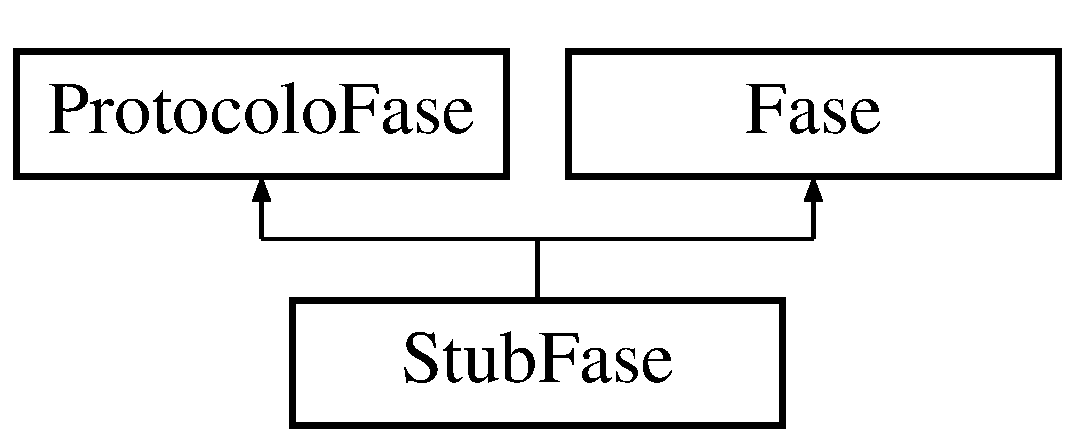
\includegraphics[height=2.000000cm]{class_stub_fase}
\end{center}
\end{figure}
\subsection*{\-Membros públicos}
\begin{DoxyCompactItemize}
\item 
\hypertarget{class_stub_fase_a7b7bcbc3c55c19fd43528d9918eb2c4e}{
void {\bfseries cadastrar} (\hyperlink{class_fase}{\-Fase})}
\label{class_stub_fase_a7b7bcbc3c55c19fd43528d9918eb2c4e}

\item 
\hypertarget{class_stub_fase_a2bd2b8628c5afb67b11e4803c79bc474}{
void {\bfseries atualizar} (\hyperlink{class_fase}{\-Fase})}
\label{class_stub_fase_a2bd2b8628c5afb67b11e4803c79bc474}

\end{DoxyCompactItemize}
\subsection*{\-Atributos \-Públicos}
\begin{DoxyCompactItemize}
\item 
\hypertarget{class_stub_fase_a21d3b78f971aecfe30d681e224dbf6da}{
string {\bfseries codigo\-Saida}}
\label{class_stub_fase_a21d3b78f971aecfe30d681e224dbf6da}

\item 
\hypertarget{class_stub_fase_a0faf568406692a8a6ac2e94654ab64d3}{
unsigned int {\bfseries tempo\-Efetivo}}
\label{class_stub_fase_a0faf568406692a8a6ac2e94654ab64d3}

\item 
\hypertarget{class_stub_fase_a7bb522d8e2941084d368a8a7098e2c9a}{
unsigned int {\bfseries tempo\-Estimado}}
\label{class_stub_fase_a7bb522d8e2941084d368a8a7098e2c9a}

\end{DoxyCompactItemize}


\subsection{\-Descrição detalhada}
\-Classe que simula a logica de negocio de \hyperlink{class_fase}{\-Fase}. 

\-Simula acoes como cadastrar e atualizar \hyperlink{class_fase}{\-Fase}, alem de apresentar tempo efetivo e tempo estimado do projeto 

\-A documentação para esta classe foi gerada a partir do seguinte ficheiro\-:\begin{DoxyCompactItemize}
\item 
\-Stubs.\-h\end{DoxyCompactItemize}

\hypertarget{class_stub_metrica}{
\section{\-Referência à classe \-Stub\-Metrica}
\label{class_stub_metrica}\index{\-Stub\-Metrica@{\-Stub\-Metrica}}
}


\-Classe que simula servicos da classe \hyperlink{class_protocolo_metrica}{\-Protocolo\-Metrica}.  




{\ttfamily \#include $<$\-Stubs.\-h$>$}

\-Diagrama de heranças da classe \-Stub\-Metrica\begin{figure}[H]
\begin{center}
\leavevmode
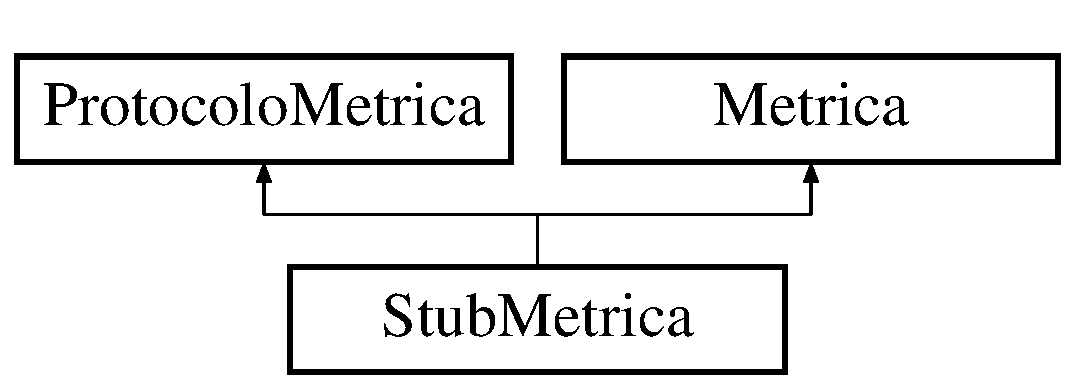
\includegraphics[height=2.000000cm]{class_stub_metrica}
\end{center}
\end{figure}
\subsection*{\-Membros públicos}
\begin{DoxyCompactItemize}
\item 
\hypertarget{class_stub_metrica_af6353cda0437cf6b6dfd7d58c77922cc}{
void {\bfseries numero\-\_\-linhas} (\hyperlink{class_metrica}{\-Metrica})}
\label{class_stub_metrica_af6353cda0437cf6b6dfd7d58c77922cc}

\item 
\hypertarget{class_stub_metrica_a5442ef24dda922c46f78033822624a80}{
void {\bfseries tempo\-\_\-gasto\-\_\-projeto} (\hyperlink{class_metrica}{\-Metrica})}
\label{class_stub_metrica_a5442ef24dda922c46f78033822624a80}

\item 
\hypertarget{class_stub_metrica_a9df31e256e503d12aa703ece9908d485}{
void {\bfseries tempo\-\_\-gasto\-\_\-modulo} (\hyperlink{class_metrica}{\-Metrica})}
\label{class_stub_metrica_a9df31e256e503d12aa703ece9908d485}

\item 
\hypertarget{class_stub_metrica_a0a9c7633fc63cf5aa6702cab10fd59e3}{
void {\bfseries produtividade\-\_\-projeto} (\hyperlink{class_metrica}{\-Metrica})}
\label{class_stub_metrica_a0a9c7633fc63cf5aa6702cab10fd59e3}

\item 
\hypertarget{class_stub_metrica_afcd0d5c8ccac15c9f21f4d246204d139}{
void {\bfseries produtividade\-\_\-modulo} (\hyperlink{class_metrica}{\-Metrica})}
\label{class_stub_metrica_afcd0d5c8ccac15c9f21f4d246204d139}

\item 
\hypertarget{class_stub_metrica_a7b202c1bdfe14be9ffd6cea862aa171e}{
void {\bfseries nota} (\hyperlink{class_metrica}{\-Metrica})}
\label{class_stub_metrica_a7b202c1bdfe14be9ffd6cea862aa171e}

\item 
\hypertarget{class_stub_metrica_a8b977e3b6f04bd72982fe4ece27760d2}{
void {\bfseries tamanho\-\_\-medio} (\hyperlink{class_metrica}{\-Metrica})}
\label{class_stub_metrica_a8b977e3b6f04bd72982fe4ece27760d2}

\item 
\hypertarget{class_stub_metrica_a99ba0d17626dae3f70102f7cddf4726a}{
void {\bfseries produtividade\-\_\-media} (\hyperlink{class_metrica}{\-Metrica})}
\label{class_stub_metrica_a99ba0d17626dae3f70102f7cddf4726a}

\end{DoxyCompactItemize}
\subsection*{\-Atributos \-Públicos}
\begin{DoxyCompactItemize}
\item 
\hypertarget{class_stub_metrica_ad3b26cd73c746e124cc8dcbae5fe6edf}{
string {\bfseries matricula\-Saida}}
\label{class_stub_metrica_ad3b26cd73c746e124cc8dcbae5fe6edf}

\item 
\hypertarget{class_stub_metrica_a5b84795353049d9b12c252d77c837a54}{
string {\bfseries codigo\-Saida}}
\label{class_stub_metrica_a5b84795353049d9b12c252d77c837a54}

\end{DoxyCompactItemize}


\subsection{\-Descrição detalhada}
\-Classe que simula servicos da classe \hyperlink{class_protocolo_metrica}{\-Protocolo\-Metrica}. 

\-Realiza acoes como mostrar numero de linhas, tempo gasto do projeto, tempo gasto do modulo, produtividade do modulo, notas, tamanho medio e produtividade media de \hyperlink{class_metrica}{\-Metrica} 

\-A documentação para esta classe foi gerada a partir do seguinte ficheiro\-:\begin{DoxyCompactItemize}
\item 
\-Stubs.\-h\end{DoxyCompactItemize}

\hypertarget{class_stub_modulo}{
\section{\-Referência à classe \-Stub\-Modulo}
\label{class_stub_modulo}\index{\-Stub\-Modulo@{\-Stub\-Modulo}}
}


\-Classe que simula servicos da classe \hyperlink{class_protocolo_projeto}{\-Protocolo\-Projeto}.  




{\ttfamily \#include $<$\-Stubs.\-h$>$}

\-Diagrama de heranças da classe \-Stub\-Modulo\begin{figure}[H]
\begin{center}
\leavevmode
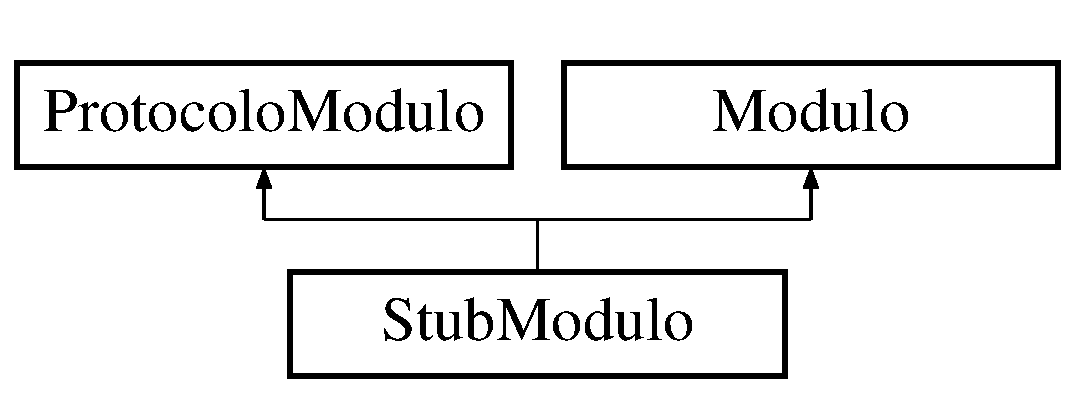
\includegraphics[height=2.000000cm]{class_stub_modulo}
\end{center}
\end{figure}
\subsection*{\-Membros públicos}
\begin{DoxyCompactItemize}
\item 
\hypertarget{class_stub_modulo_ad3ee153e45f91a9000ea12064d876528}{
void {\bfseries cadastrar} (\hyperlink{class_modulo}{\-Modulo})}
\label{class_stub_modulo_ad3ee153e45f91a9000ea12064d876528}

\item 
\hypertarget{class_stub_modulo_a8bb3265b52dca8f8358917b8eb5f3009}{
void {\bfseries remover} (\hyperlink{class_codigo___modulo}{\-Codigo\-\_\-\-Modulo})}
\label{class_stub_modulo_a8bb3265b52dca8f8358917b8eb5f3009}

\item 
\hypertarget{class_stub_modulo_a68c0ce9a1a91220283cdb568241bba8c}{
void {\bfseries pesquisar} (\hyperlink{class_modulo}{\-Modulo} $\ast$)}
\label{class_stub_modulo_a68c0ce9a1a91220283cdb568241bba8c}

\item 
\hypertarget{class_stub_modulo_a4997adf1d294eef4a3bd955a4d51cf9a}{
void {\bfseries atualizar} (\hyperlink{class_modulo}{\-Modulo})}
\label{class_stub_modulo_a4997adf1d294eef4a3bd955a4d51cf9a}

\end{DoxyCompactItemize}
\subsection*{\-Atributos \-Públicos}
\begin{DoxyCompactItemize}
\item 
\hypertarget{class_stub_modulo_a9bc8593126dab6fb368bdf6b9765762b}{
string {\bfseries codigo\-Saida}}
\label{class_stub_modulo_a9bc8593126dab6fb368bdf6b9765762b}

\item 
\hypertarget{class_stub_modulo_a860047f783bb6c9a4a9b701392fc442f}{
string {\bfseries nome\-Saida}}
\label{class_stub_modulo_a860047f783bb6c9a4a9b701392fc442f}

\item 
\hypertarget{class_stub_modulo_a7bb8a0cad02c80cf0f968f4783e2eba4}{
unsigned int {\bfseries tamanho\-Saida}}
\label{class_stub_modulo_a7bb8a0cad02c80cf0f968f4783e2eba4}

\end{DoxyCompactItemize}


\subsection{\-Descrição detalhada}
\-Classe que simula servicos da classe \hyperlink{class_protocolo_projeto}{\-Protocolo\-Projeto}. 

\-Simula acoes como cadastrar, remover, pesquisar e atualizar \hyperlink{class_projeto}{\-Projeto} 

\-A documentação para esta classe foi gerada a partir do seguinte ficheiro\-:\begin{DoxyCompactItemize}
\item 
\-Stubs.\-h\end{DoxyCompactItemize}

\hypertarget{class_stub_projeto}{
\section{\-Referência à classe \-Stub\-Projeto}
\label{class_stub_projeto}\index{\-Stub\-Projeto@{\-Stub\-Projeto}}
}


\-Classe que simula servicos da classe \hyperlink{class_protocolo_projeto}{\-Protocolo\-Projeto}.  




{\ttfamily \#include $<$\-Stubs.\-h$>$}

\-Diagrama de heranças da classe \-Stub\-Projeto\begin{figure}[H]
\begin{center}
\leavevmode
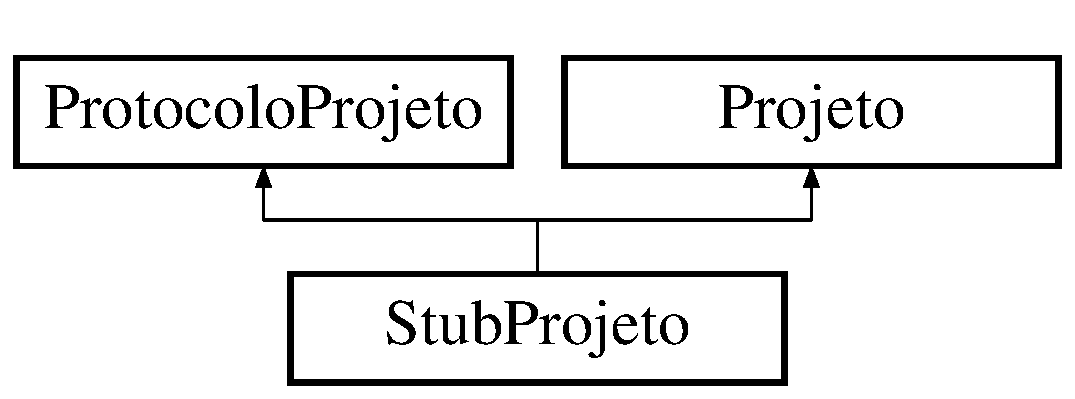
\includegraphics[height=2.000000cm]{class_stub_projeto}
\end{center}
\end{figure}
\subsection*{\-Membros públicos}
\begin{DoxyCompactItemize}
\item 
\hypertarget{class_stub_projeto_aeaf8872b472ce840a202f28a85b3e3df}{
void {\bfseries cadastrar} (\hyperlink{class_projeto}{\-Projeto})}
\label{class_stub_projeto_aeaf8872b472ce840a202f28a85b3e3df}

\item 
\hypertarget{class_stub_projeto_aad62ccaefc75730981af138f3402b78c}{
void {\bfseries remover} (\hyperlink{class_codigo___projeto}{\-Codigo\-\_\-\-Projeto})}
\label{class_stub_projeto_aad62ccaefc75730981af138f3402b78c}

\item 
\hypertarget{class_stub_projeto_a205f75c241e3c49ea66f3930cb5c458e}{
void {\bfseries pesquisar} (\hyperlink{class_projeto}{\-Projeto} $\ast$)}
\label{class_stub_projeto_a205f75c241e3c49ea66f3930cb5c458e}

\item 
\hypertarget{class_stub_projeto_a4bf3a817d152ab3461eda3a48defbf56}{
void {\bfseries atualizar} (\hyperlink{class_projeto}{\-Projeto})}
\label{class_stub_projeto_a4bf3a817d152ab3461eda3a48defbf56}

\end{DoxyCompactItemize}
\subsection*{\-Atributos \-Públicos}
\begin{DoxyCompactItemize}
\item 
\hypertarget{class_stub_projeto_ab36205997d647207e3079facb63d5b13}{
string {\bfseries matricula\-Saida}}
\label{class_stub_projeto_ab36205997d647207e3079facb63d5b13}

\item 
\hypertarget{class_stub_projeto_a66a8eadef8b6bcea586b90f2c19a25f2}{
string {\bfseries codigo\-Saida}}
\label{class_stub_projeto_a66a8eadef8b6bcea586b90f2c19a25f2}

\item 
\hypertarget{class_stub_projeto_a3396b49699e29793ef6beed7307ff6ca}{
unsigned int {\bfseries data\-Inicio\-Saida}}
\label{class_stub_projeto_a3396b49699e29793ef6beed7307ff6ca}

\item 
\hypertarget{class_stub_projeto_a6c86a70a9d3d9dacc6be8bb5fb1f8777}{
unsigned int {\bfseries data\-Termino\-Saida}}
\label{class_stub_projeto_a6c86a70a9d3d9dacc6be8bb5fb1f8777}

\item 
\hypertarget{class_stub_projeto_a87f19311fdb5a96fb3d209e2361cd6c1}{
unsigned int {\bfseries nota\-Saida}}
\label{class_stub_projeto_a87f19311fdb5a96fb3d209e2361cd6c1}

\end{DoxyCompactItemize}


\subsection{\-Descrição detalhada}
\-Classe que simula servicos da classe \hyperlink{class_protocolo_projeto}{\-Protocolo\-Projeto}. 

\-Simula acoes como cadastrar, remover, pesquisar e atualizar \hyperlink{class_projeto}{\-Projeto} 

\-A documentação para esta classe foi gerada a partir do seguinte ficheiro\-:\begin{DoxyCompactItemize}
\item 
\-Stubs.\-h\end{DoxyCompactItemize}

\hypertarget{class_tamanho}{
\section{\-Referência da \-Classe \-Tamanho}
\label{class_tamanho}\index{\-Tamanho@{\-Tamanho}}
}


\-Classe que representa o dominio \hyperlink{class_tamanho}{\-Tamanho}.  




{\ttfamily \#include $<$\-Dominios.\-h$>$}

\subsection*{\-Métodos \-Públicos}
\begin{DoxyCompactItemize}
\item 
\hypertarget{class_tamanho_a63541f3ebe1209729030e17b6a21236c}{
{\bfseries \-Tamanho} (unsigned int)  throw (invalid\-\_\-argument)}
\label{class_tamanho_a63541f3ebe1209729030e17b6a21236c}

\item 
void \hyperlink{class_tamanho_afb80c548279d5baa4f0ef163f7f564d0}{set\-Valor} (const unsigned int \&)  throw (invalid\-\_\-argument)
\begin{DoxyCompactList}\small\item\em \-Seta o valor de \hyperlink{class_tamanho}{\-Tamanho}. \end{DoxyCompactList}\item 
unsigned int \hyperlink{class_tamanho_a0150e086c4b3d37b9d98e34c34532a10}{get\-Valor} () const 
\begin{DoxyCompactList}\small\item\em \-Retorna o valor de \hyperlink{class_tamanho}{\-Tamanho}. \end{DoxyCompactList}\end{DoxyCompactItemize}


\subsection{\-Descrição \-Detalhada}
\-Classe que representa o dominio \hyperlink{class_tamanho}{\-Tamanho}. 

\-Armazena os atributos de \hyperlink{class_tamanho}{\-Tamanho} \-Em \-Linhas \-De \-Codigo apos validacao\-: valor de 0 a 1000 

\subsection{\-Métodos}
\hypertarget{class_tamanho_a0150e086c4b3d37b9d98e34c34532a10}{
\index{\-Tamanho@{\-Tamanho}!get\-Valor@{get\-Valor}}
\index{get\-Valor@{get\-Valor}!Tamanho@{\-Tamanho}}
\subsubsection[{get\-Valor}]{\setlength{\rightskip}{0pt plus 5cm}unsigned int \-Tamanho\-::get\-Valor (
\begin{DoxyParamCaption}
{}
\end{DoxyParamCaption}
) const\hspace{0.3cm}{\ttfamily  \mbox{[}inline\mbox{]}}}}
\label{class_tamanho_a0150e086c4b3d37b9d98e34c34532a10}


\-Retorna o valor de \hyperlink{class_tamanho}{\-Tamanho}. 

\begin{DoxyReturn}{\-Retorna}
valor 
\end{DoxyReturn}
\hypertarget{class_tamanho_afb80c548279d5baa4f0ef163f7f564d0}{
\index{\-Tamanho@{\-Tamanho}!set\-Valor@{set\-Valor}}
\index{set\-Valor@{set\-Valor}!Tamanho@{\-Tamanho}}
\subsubsection[{set\-Valor}]{\setlength{\rightskip}{0pt plus 5cm}void \-Tamanho\-::set\-Valor (
\begin{DoxyParamCaption}
\item[{const unsigned int \&}]{valor}
\end{DoxyParamCaption}
)  throw (invalid\-\_\-argument)\hspace{0.3cm}{\ttfamily  \mbox{[}inline\mbox{]}}}}
\label{class_tamanho_afb80c548279d5baa4f0ef163f7f564d0}


\-Seta o valor de \hyperlink{class_tamanho}{\-Tamanho}. 


\begin{DoxyParams}{\-Parâmetros}
{\em valor} & \\
\hline
\end{DoxyParams}


\-A documentação para esta classe foi gerada a partir do seguinte arquivo\-:\begin{DoxyCompactItemize}
\item 
header/\-Dominios.\-h\end{DoxyCompactItemize}

\hypertarget{class_tempo}{
\section{\-Referência à classe \-Tempo}
\label{class_tempo}\index{\-Tempo@{\-Tempo}}
}


\-Classe que representa o dominio \hyperlink{class_tempo}{\-Tempo}.  




{\ttfamily \#include $<$\-Dominios.\-h$>$}

\subsection*{\-Membros públicos}
\begin{DoxyCompactItemize}
\item 
\hypertarget{class_tempo_adaa477ff29f28230aac7f70c32ac792b}{
{\bfseries \-Tempo} (string)  throw (invalid\-\_\-argument)}
\label{class_tempo_adaa477ff29f28230aac7f70c32ac792b}

\item 
void \hyperlink{class_tempo_aa692776272a35f0457c3610fbca8853e}{set\-Valor} (const string \&)  throw (invalid\-\_\-argument)
\begin{DoxyCompactList}\small\item\em \-Seta o valor de \hyperlink{class_tempo}{\-Tempo}. \end{DoxyCompactList}\item 
string \hyperlink{class_tempo_a52d19fafeba9848f5127906e0308c0b9}{get\-Valor} () const 
\begin{DoxyCompactList}\small\item\em \-Retorna o valor de \hyperlink{class_tamanho}{\-Tamanho}. \end{DoxyCompactList}\end{DoxyCompactItemize}


\subsection{\-Descrição detalhada}
\-Classe que representa o dominio \hyperlink{class_tempo}{\-Tempo}. 

\-Armazena os atributos de \hyperlink{class_tempo}{\-Tempo} apos validacao\-: valor de 0 a 2000 

\subsection{\-Documentação dos métodos}
\hypertarget{class_tempo_a52d19fafeba9848f5127906e0308c0b9}{
\index{\-Tempo@{\-Tempo}!get\-Valor@{get\-Valor}}
\index{get\-Valor@{get\-Valor}!Tempo@{\-Tempo}}
\subsubsection[{get\-Valor}]{\setlength{\rightskip}{0pt plus 5cm}string \-Tempo\-::get\-Valor (
\begin{DoxyParamCaption}
{}
\end{DoxyParamCaption}
) const\hspace{0.3cm}{\ttfamily  \mbox{[}inline\mbox{]}}}}
\label{class_tempo_a52d19fafeba9848f5127906e0308c0b9}


\-Retorna o valor de \hyperlink{class_tamanho}{\-Tamanho}. 

\begin{DoxyReturn}{\-Retorna}
valor 
\end{DoxyReturn}
\hypertarget{class_tempo_aa692776272a35f0457c3610fbca8853e}{
\index{\-Tempo@{\-Tempo}!set\-Valor@{set\-Valor}}
\index{set\-Valor@{set\-Valor}!Tempo@{\-Tempo}}
\subsubsection[{set\-Valor}]{\setlength{\rightskip}{0pt plus 5cm}void \-Tempo\-::set\-Valor (
\begin{DoxyParamCaption}
\item[{const string \&}]{valor}
\end{DoxyParamCaption}
)  throw (invalid\-\_\-argument)\hspace{0.3cm}{\ttfamily  \mbox{[}inline\mbox{]}}}}
\label{class_tempo_aa692776272a35f0457c3610fbca8853e}


\-Seta o valor de \hyperlink{class_tempo}{\-Tempo}. 


\begin{DoxyParams}{\-Parâmetros}
{\em valor} & \\
\hline
\end{DoxyParams}


\-A documentação para esta classe foi gerada a partir do seguinte ficheiro\-:\begin{DoxyCompactItemize}
\item 
\-Dominios.\-h\end{DoxyCompactItemize}

\printindex
\end{document}
